% arara: pdflatex
% arara: pdflatex
% arara: pdflatex

% options:
% thesis=B bachelor's thesis
% thesis=M master's thesis
% czech thesis in Czech language
% slovak thesis in Slovak language
% english thesis in English language
% hidelinks remove colour boxes around hyperlinks

\documentclass[thesis=B,english]{FITthesis}[2019/12/23]

\usepackage[utf8]{inputenc} % LaTeX source encoded as UTF-8
\usepackage[style=iso-numeric]{biblatex}

\usepackage{csquotes} %fit template is probably loading polyglossia and it throws error without csquotes package loaded

\usepackage{pgfplots}
\pgfplotsset{compat=1.17}
\usepgfplotslibrary{statistics}
\usepackage{pgf-pie}

\addbibresource{bibliography.bib}

\usepackage{hyperref}
\emergencystretch=1em %solves some overfull hboxes

\usepackage{graphicx}
\graphicspath{ {./pictures/} }
\usepackage{minted} %source code highlighting

\usepackage{subcaption}
\usepackage{amsmath} %cases v matematickem prostredi, vice radek (x = 1 jestliže neco, x = 0 jinak)
\usepackage{gensymb} %nutné například pro symbol stupně
\usepackage{todonotes}
\usepackage{placeins} %needed to create barriers for floating environments


\usepackage{mathrsfs} %math font
\usepackage{amssymb} %math fonts(eg: real number font) %additional math symbols

% \usepackage{amsmath} %advanced maths

\usepackage{dirtree} %directory tree visualisation

% % list of acronyms
% \usepackage[acronym,nonumberlist,toc,numberedsection=autolabel]{glossaries}
% \iflanguage{czech}{\renewcommand*{\acronymname}{Seznam pou{\v z}it{\' y}ch zkratek}}{}
% \makeglossaries

\newcommand{\tg}{\mathop{\mathrm{tg}}} %cesky tangens
\newcommand{\cotg}{\mathop{\mathrm{cotg}}} %cesky cotangens

% % % % % % % % % % % % % % % % % % % % % % % % % % % % % %
% ODTUD DAL VSE ZMENTE
% % % % % % % % % % % % % % % % % % % % % % % % % % % % % %

\department{Department of Software Engineering}
\title{Urban scene recognition and editing II.}
\authorGN{Pavel} %(křestní) jméno (jména) autora
\authorFN{Kříž} %příjmení autora
\authorWithDegrees{Pavel Kříž} %jméno autora včetně současných akademických titulů
\author{Pavel Kříž} %jméno autora bez akademických titulů
\supervisor{Ing. Radek Richtr, Ph.D.}
\acknowledgements{I want to thank my bachelor thesis supervisor Ing. Radek Richtr, Ph.D. for how he led me to the solutions and gave me answers for my questions. I also want to thank Ing. Jiří Chludil for helping me understand all the technical specifications regarding the \textit{Dowry Towns of Bohemians Queens} project that I needed. Last but not least, I want to thank my father and sister who helped me to correct my grammar and improve other features of my text.}


\abstractCS{Naše práce je součástí projektu \textit{Věnná města českých královen}, jehož cílem je přiblížit historii široké veřejnosti za použití moderních technologií, jako je rozšířená realita. K tomu slouží aplikace pro mobilní zařízení se systémem Android, která za běhu zobrazuje historické prvky do scény fotoaparátu. Tato práce se na jejím vývoji podílí tím, že navrhuje lokalizační řešení pro aplikaci za použití obrazových a geolokačních dat. V úvodu jsou popsány a analyzovány potenciálně použitelné technologie a práce, které v rámci uvedeného projektu naší práci předcházely. Tato práce pak konkrétně navazuje na bakalářskou práci \textit{Rozpoznávání a editace urbanistické scény}. Výsledky předcházející práce jsme adaptovali pro potřeby naší práce, ve které jsme realizovali nový pokročilejší prototyp založený na výpočtu globální polohy zařízení. Nový prototyp je pak testován na funkčnost i na praktickou použitelnost s ohledem na hardwarové možnosti zařízení a porovnáván se stávajícími možnostmi zařízení. V závěru práce je posuzováno zapojení prototypu do mobilní aplikace projektu a jsou předloženy podněty pro další budoucí vývoj.}


\abstractEN{Our work is part of the \textit{Dowry Cities of Czech Queens} project, which aims to bring history closer to the general public using modern technologies such as augmented reality. This is done using an application for Android mobile devices, which displays historical elements in the camera scene at runtime. This work contributes to its development by proposing a localisation solution for the application using image and geolocation data. The introduction describes and analyses potentially applicable technologies and works that preceded our work within the project. This work then specifically follows on from the bachelor's thesis \textit{Recognition and Editing of the Urban Scene}. We adapted the results of the previous work for the needs of our work, in which we implemented a new more advanced prototype based on the calculation of the global position of the device. The new prototype is then tested for functionality and practical applicability with respect to the hardware capabilities of the device and compared with existing device capabilities. At the end of the work, the involvement of the prototype in the mobile application of the project is proposed and suggestions for further future development are presented.}


\placeForDeclarationOfAuthenticity{Prague}
\declarationOfAuthenticityOption{5} %volba Prohlášení (číslo 1-6)
\keywordsCS{počítačové vidění, lokalizace, rozšířená realita, OpenCV, obrazové příznaky, Věnná města českých královen}
\keywordsEN{computer vision, localisation, augmented reality, OpenCV, image features, Dowry Towns of Bohemian Queens}
% \website{http://site.example/thesis} %volitelná URL práce, objeví se v tiráži - úplně odstraňte, nemáte-li URL práce

\begin{document}

% \newacronym{CVUT}{{\v C}VUT}{{\v C}esk{\' e} vysok{\' e} u{\v c}en{\' i} technick{\' e} v Praze}
% \newacronym{FIT}{FIT}{Fakulta informa{\v c}n{\' i}ch technologi{\' i}}

\begin{introduction}
    Augmented reality is a term for the method of extending a real world image by some computer-generated content. The difference of augmented reality to virtual reality is that the immersion to the computer-generated content is significantly lower and instead of creating a new world it rather extends the already existing one. Nowadays, the most common form of augmented reality is inserting content into the image of a smartphone camera in real time. In the \textit{Dowry Towns of Bohemians queens} project one of the goals is to create a mobile application that will allow to display 3D models in the scene of the mobile device. The application will display models of historical buildings and other objects. By doing that will the application create a view to the history of the place where the application will be used. Such a window to the history will allow seeing buildings that were already demolished or their look was changed significantly in their original form at the original places.
    
    In that point occurs a problem for which a solution has to be found. The historical buildings cannot be displayed randomly all over the place in the scene of the smartphone camera. The buildings have to be placed on the exactly determined positions where they have stood before so the display has a historical value and accuracy. In order to place the buildings into the correct position the precise location of the smartphone has to be known. Nowadays positioning (GPS) sensors guarantee accuracy in meters and sometimes they lose the location accuracy completely. But the accuracy of the positioning is key to place the buildings in correct positions and a few meters make a big difference especially in case of smaller buildings.
    
    The solution of that problem is searched in the area of computer vision. When the building and its location were recognised in the image of the smartphone camera, the location towards the building could be calculated. Prototype solution of the image recognition was already created in the preceding thesis \textit{Urban scene recognition and editing}~\cite{Sefcik2020}. But beside the solution of the image recognition it is also needed to create a solution for calculating the global location or relative location towards the recognised building.
\end{introduction}

%TODO - pridat kurzívu na nejaka mista jako zvyrazneni (takova mista v textu jsou)

%\chapter{Objectives of our thesis}
   % The main goal of our bachelor thesis is to implement a localisation algorithm using computer vision. Output of such an algorithm has to be the precise location (relative to some object or in the world coordinates). We will also work on achieving the robustness of the algorithm. Such robustness includes invariance to rotation, scale, or other variables such as weather and lighting condition. This would be done with the aim for the highest precision and efficiency of the calculation.
    %\to do[]{ja vim ze na dpr nebo kde vam tuhle kapitolu vnucuji... ale v aj to za a zni blbe a za b.. ji klidne vynechte}
    
\chapter{Research}
    In this chapter are explained the theoretical basics of the image processing that we consider to use in this project. In our project the image processing includes image pre-processing, image identification and comparison of the images based on their identification. At the end we explain the perspective-n-point problem.
    
    \section{From light to the image}
        %ZDE NAPSÁNO ŽE JE TATO SEKCE CELA ZE ŽÁRY - učebnice!!!
        In this section it is explained what colors are and how to represent them digitally or what is the image considered to be. More detailed description of the following topics can be found in the Czech learning book~\cite{ZARA2005}. This whole section is based on that book.
        \subsection{Human perception of colors}
            %V ÚVODU NAPSÁNO ŽE JE TATO SEKCE CELA ZE ŽÁRY - učebnice!!!
            All known kinds of electromagnetic radiation like x-ray, microwave or visible light are included in the electromagnetic spectrum. Specifically, visible light, also called the visible spectrum, is a radiation with wavelengths in the range of about 380 to 720 nm. Specific color is then radiation with specific wavelength from the visible spectrum. Light with wavelength about 550 nm is perceived as green and light with wavelength 720 as red. The so-called white light is then composed of rays from the entire visible spectrum (with all possible visible wavelengths). Such light is produced by the sun or a light bulb and is called neutral light (achromatic light). When light hits a surface, some rays of light are absorbed and some are reflected depending on the physical properties of the surface. The resulting composition of the reflected rays creates what we understand as color of the surface. The dominant frequency of light influences how the color is perceived by humans. For example, a color with a majority of rays with frequencies about 550 nm would be called green.

            The following terms are important for describing colors:
            
            \begin{description}
                \item[Luminance] is a physical quantity describing the amount of light.
                \item[Brightness] is a subjective perception of the light intensity.
                \item[Saturation] purity of the light color is described by this term. The tighter is the frequency spectrum of light the more saturated the color is.
                \item[Lightness] in light with some dominant frequency is the lightness, the amount of neutral light.
            \end{description}
            
            \subsubsection*{Human eye}
            Rod cells and cone cells are sort of sensors in the human eye which are responsible for perception of light and color. The rod cells are approximately ten times more sensitive to light then the cone cells and thus the rod cell's purpose is mainly to measure the luminance. The cone cells complement the rod cells in a way that they measure the colors.
            
            Each cone cell has one of three different photopigments. Each photopigment is more or less sensitive to specific wavelengths. Blue photopigment is a photopigment that is most sensitive to light rays with a wavelength about 445 nm. Green and red is then most sensitive to rays with wavelengths about 535 nm or 575 nm respectively. Green and red photopigments, compared to blue ones, are more sensitive to the whole visible spectrum. The photopigments are also not evenly distributed among the cone cells. In the eye there are the most cone cells with red photopigment, bit less with green one and the least with blue one.
            
            \subsubsection*{Color perception}
            
            In the eye, colors are perceived as three basic colors: red (\(R\)), green (\(G\)) and blue (\(B\)) but the information about the colors is delivered to the brain in different forms. In the connection between the eye and the brain, the optic nerve, the colors are combined in the following way: The color information is represented in two channels. The first one is made by the subtraction of blue from yellow \(Y - B\) and the second one by subtraction of green from red \(R - G\). There is also a third channel created as an addition of red to green \(G + R\) and the channel indicates the brightness.
            
            \subsubsection*{Eye adaptation to luminance}
            
            An important feature of the human eye is the adaptation to luminance. It is a phenomenon of perceiving the light intensity changes (seeing surfaces with different brightness in one view). The light intensity change is not perceived linearly by humans but logarithmically. Thus, the change of light intensity is perceived as bigger in lower light intensities than in the higher ones. Thanks to the luminance adaptation, the human eye is able to perceive a wide luminance range.
            
        \subsection{Representation of colors}
            %V ÚVODU NAPSÁNO ŽE JE TATO SEKCE CELA ZE ŽÁRY - učebnice!!!
            Colors are digitally represented in various ways, which are called color models. All colors that can be represented by a color model, create a color space. One of the most used color models is RGB. The name of the model is an abbreviation derived from the three colors: red, green, and blue. These colors are considered basic colors and they are defined as a specific color in the spectrum of colors visible by a human. In RGB, colors are expressed as a combination of the basic colors. RGB is an additive color model. This means that by adding intensity in each channel, we get a brighter color. So the maximum intensities of basic colors are combined to create white and the minimum intensities to create black. Value in each channel is usually represented in range \(\langle 0, 1\rangle\) as a floating-point number or it is represented as an integer in range \(\langle 0, 255\rangle\). The last case is related to the fact that the value is usually stored on 8 bits. A maximum of 256 different values can be stored on 8 bits(\(2^8 = 256\)).
            
            There are many other color models and spaces. One of them is the color space CIE 1976 L*a*b* (also called CIELAB), that is closer to how humans perceive colors than RGB. This color model also has three channels but one of them stores the lightness of the color (channel L*). The other two channels are axis in the color space, the first one is an axis that goes from green to red (channel a*), and the second one goes from blue to yellow (channel b*). There are other models similar to this one, such as the YUV color model. This color model also has three color channels (Y, U and V) from which two (U and V) determine the chrominance (color) and the third channel (Y) stores the brightness.
        %ENGLISH
        \subsection{Image}
            In society, an image is usually understood as a painting, a drawing, or what people see on the screen, or as light that comes into the human eye. Mathematically, however, we can define an image with a continuous function \(f\) with two variables \(x\) and \(y\), \(x,y \in R\). Such a function is called an image function and can be defined as follows:
            %
            \begin{equation}
                z = f(x,y) \enspace .
            \end{equation}
            %
            Such a function considers the infinite size of the image, which is not practical. Finite image function with range \(I\) within some specific boundaries \(\langle x_{min},x_{max}\rangle\) and \(\langle y_{min},y_{max}\rangle\) can be defined as follows:
            %
            \begin{equation}
                f: (\langle x_{min},x_{max}\rangle \times \langle y_{min},y_{max}\rangle )\to I \enspace .
            \end{equation}
            %
            To represent the image digitally, the variables \(x, y\) have to be integer numbers. For discrete image functions, the value \(z\) is called \emph{pixel} (picture element). It is also important to mention that the value \(z\) does not have to be a number. In the case of RGB, the value \(z\) would be a vector made of three numbers.
            
    \section{Image pre-processing}
        It is appropriate to think about some pre-processing of the image before the main image processing. In our case, such pre-processing means to put the image in a state in which the undesirable influences are diminished as much as possible. Ideally, the image should be in the same state after the pre-processing independently on the conditions in which the image was taken.
        
        \subsection{Gamma correction}
            % specifikovat take gama kódování a dekódování
            % rict o tom ze se casto k ulozeni obrazu pouzit gama kódování a pak je ten barevný prostor nelinearni
            Gamma correction is how is called a following non-linear operation~\cite{McHughc20052020}:
            %
            \begin{equation}
                            V' = V^{\gamma} \enspace ,
            \end{equation}\label{eq:gamma}
            %
            where \(V'\) is the output and \(V\) is the input and \(\gamma\) is some real number. If \(\gamma < 1\), then such an operation is called gamma compression and the \(\gamma\) is called  \emph{encoding gamma}. If \(\gamma > 1\), the operation is then called gamma expansion and the \(\gamma\) is called  \emph{decoding gamma}. Examples of some gamma corrections may be seen in figure~\ref{fig:gamaKorekce}.

            \begin{figure}
                \centering
                %pgfplots inside tikz environment
                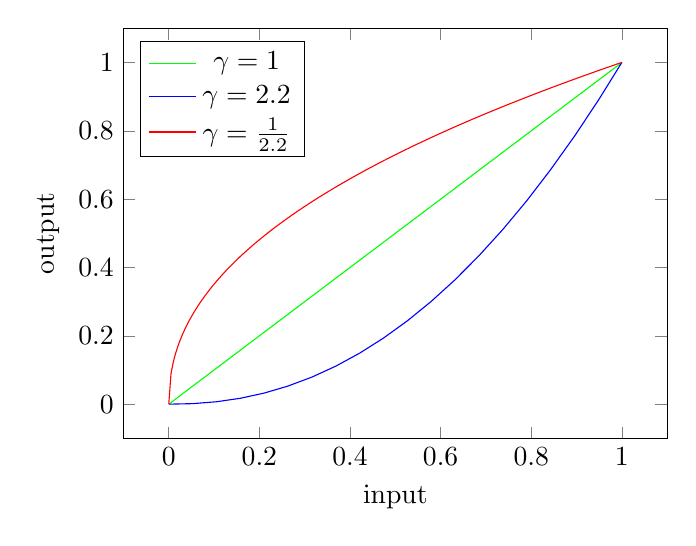
\begin{tikzpicture}
                    \begin{axis}[
                        width = 0.7\linewidth,
                        height = 0.56\linewidth,
                        legend pos = north west,
                        xlabel = input,
                        ylabel = output]
                        \addplot[domain=0:1, samples=2, color=green]{x};
                        \addlegendentry{\(\gamma = 1\)}
                        \addplot[domain=0:1, samples=20, color=blue]{x^2.2};
                        \addlegendentry{\(\gamma = 2.2\)}
                        \addplot[domain=0:1, samples=200, color=red]{x^(1/2.2)};
                        \addlegendentry{\(\gamma = \frac{1}{2.2}\)}
                      \end{axis}
                \end{tikzpicture}
                \caption{Gamma corrections examples with different gamma values}
                \label{fig:gamaKorekce}
            \end{figure}
            
            As mentioned above, the luminance is not perceived linearly by the human eye, but logarithmically, so the human eye is more sensitive to changes in darker tones of colors in comparison to lighter ones. Therefore, gamma correction is used. When the data is stored using gamma compression, then more possible values are given for darker tones. This processing has the advantage that only 8 bits instead of 11 are needed to store the same amount in the spectrum of dark shades, while maintaining the same visual quality. But in the end it is needed to transfer the data back to the linear space by processing all the values with the gamma expansion~\cite{McHughc20052020}.
            
        \subsection{Converting image to grayscale}
            There are several color models that have one channel determining the luminance of the color. Such color models are YUV for example. When the Y channel is separated, a grayscale image is created. But not all color models have such simple conversion.
            
            When converting colors from the RGB color space, it is important to know that different colors contribute to the perceiving of the brightness of the color with different amounts. This is due to the distribution of photopigments among the phone cells, as explained above. Thus, when the colors are converted, specific weights are used in a way that gives us the following formula~\cite{Poynton28November2006}:
            %
            \begin{equation}
                Y_{lin} = 0.2126 \cdot R_{lin} + 0.7152 \cdot G_{lin} + 0.0722 \cdot B_{lin} \enspace ,
            \end{equation} \label{eq:weightedRGBtoGrey}
            %
            where \(Y_{lin}\) a \(R_{lin}, G_{lin}, B_{lin}\) are values of lightness of the basic colors stored in the linear space.
            
            If the colors are stored in gamma compressed space, the values are first transferred back to the linear space by using gamma expansion. Then is done the conversion to the grayscale and the shades of gray are gamma compressed again~\cite{NPlDwZHLJCEKbaXV}. Different weights may be used for the conversion for different standards. The weights are also not scientifically determined, but determined experimentally, so they provide satisfactory results. For simplicity, a linear conversion from a non-linear color space to non-linear space of shades of grey is sometimes used~\cite{Poynton28November2006}.
            
        \subsection{Histogram equalisation}
            Histogram equalisation is a method to change the global contrast in an image. A histogram is a distribution of the values in the image. Contrast can be explained as the difference of values between two objects (points, areas or lines)~\cite{X3IOSjMG1S81OB7w}. If the contrast is too low, it is difficult to distinguish two objects in image, see the picture~\ref{subFig:lowContrastCows} with the histogram in the image~\ref{subFig:lowContrastCowsHist}. The values are crammed in the middle of the histogram, leading to smaller differences between the values in the image. After applying the equalisation, the values are evenly distributed among the range of values, see the picture~\ref{subFig:equalizedCows} with the histogram~\ref{subFig:equalizedCowsHist}. The image with an equalised histogram has a higher contrast than the original image. Increasing the contrast helps the texture and objects in the image to stand out more.
            
            \begin{figure}
                \centering
                \newcommand \histEqImagesHeight{ \linewidth}
                \begin{subfigure}{0.39\linewidth}
                    \centering
                    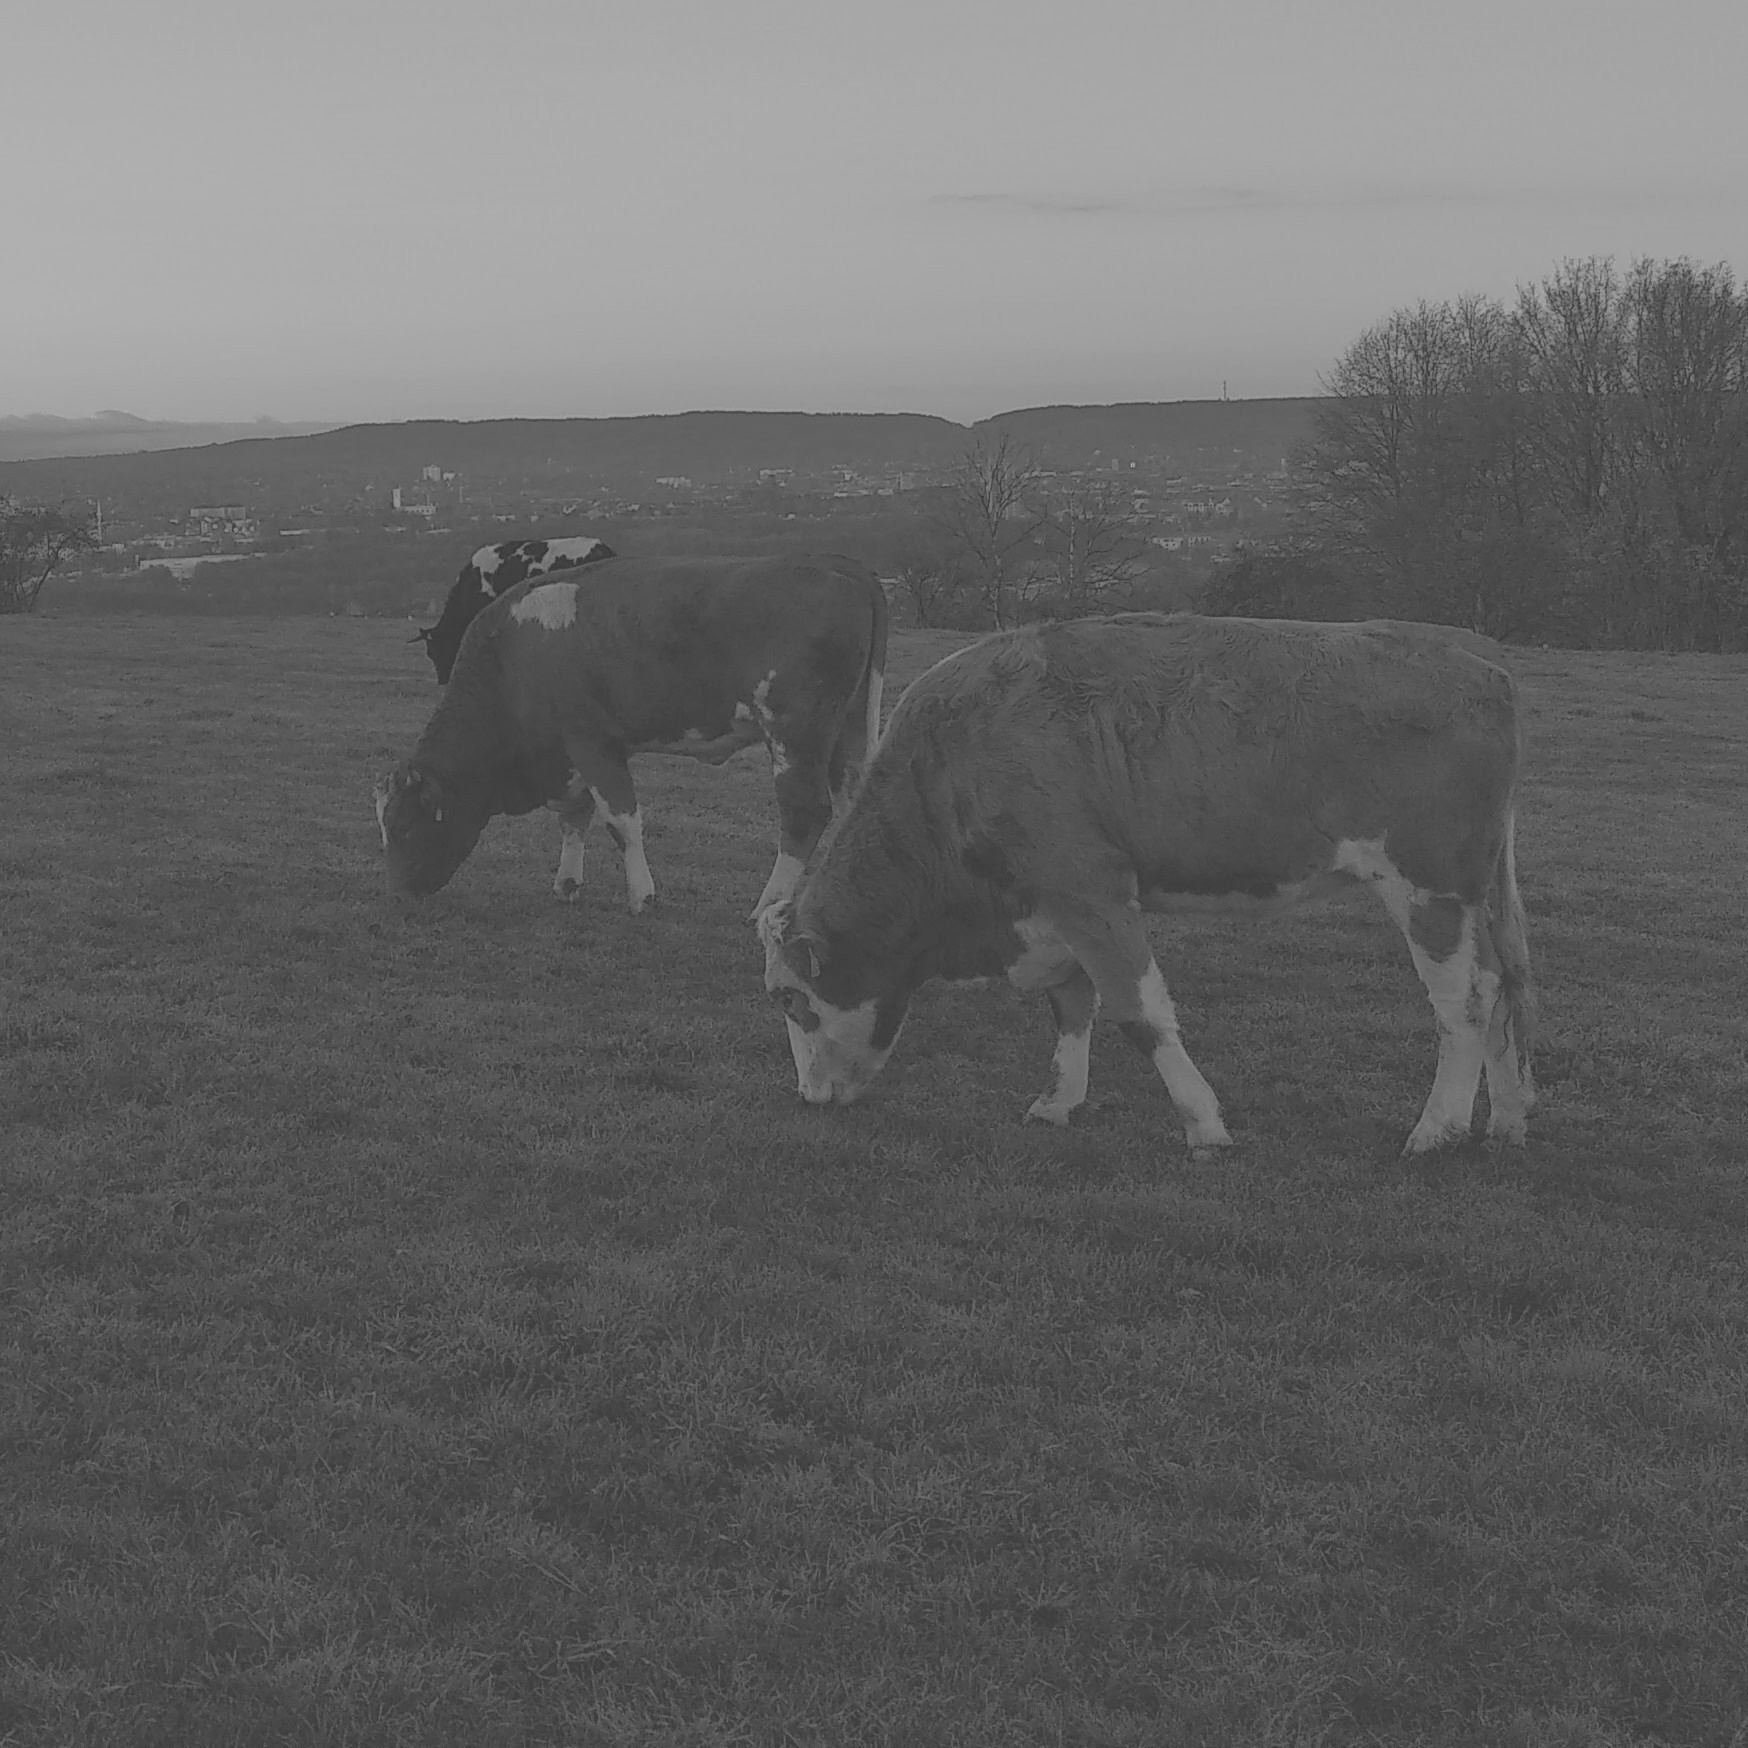
\includegraphics[
                        width=\linewidth,
                        height=\histEqImagesHeight]{lowContrastCows.jpg}
                    \caption{Original image}
                    \label{subFig:lowContrastCows}
                \end{subfigure}
                \begin{subfigure}{0.39\linewidth}
                    \centering
                    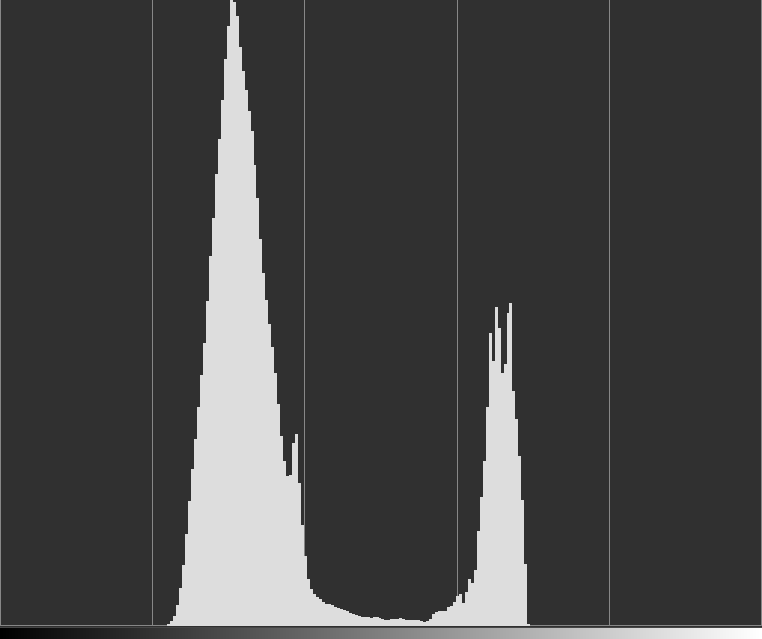
\includegraphics[
                        width=\linewidth,
                        height=\histEqImagesHeight]{lowContrastCowsHist.png}
                    \caption{Original histogram}
                    \label{subFig:lowContrastCowsHist}
                \end{subfigure}
                \\
                \begin{subfigure}{0.39\linewidth}
                    \centering
                    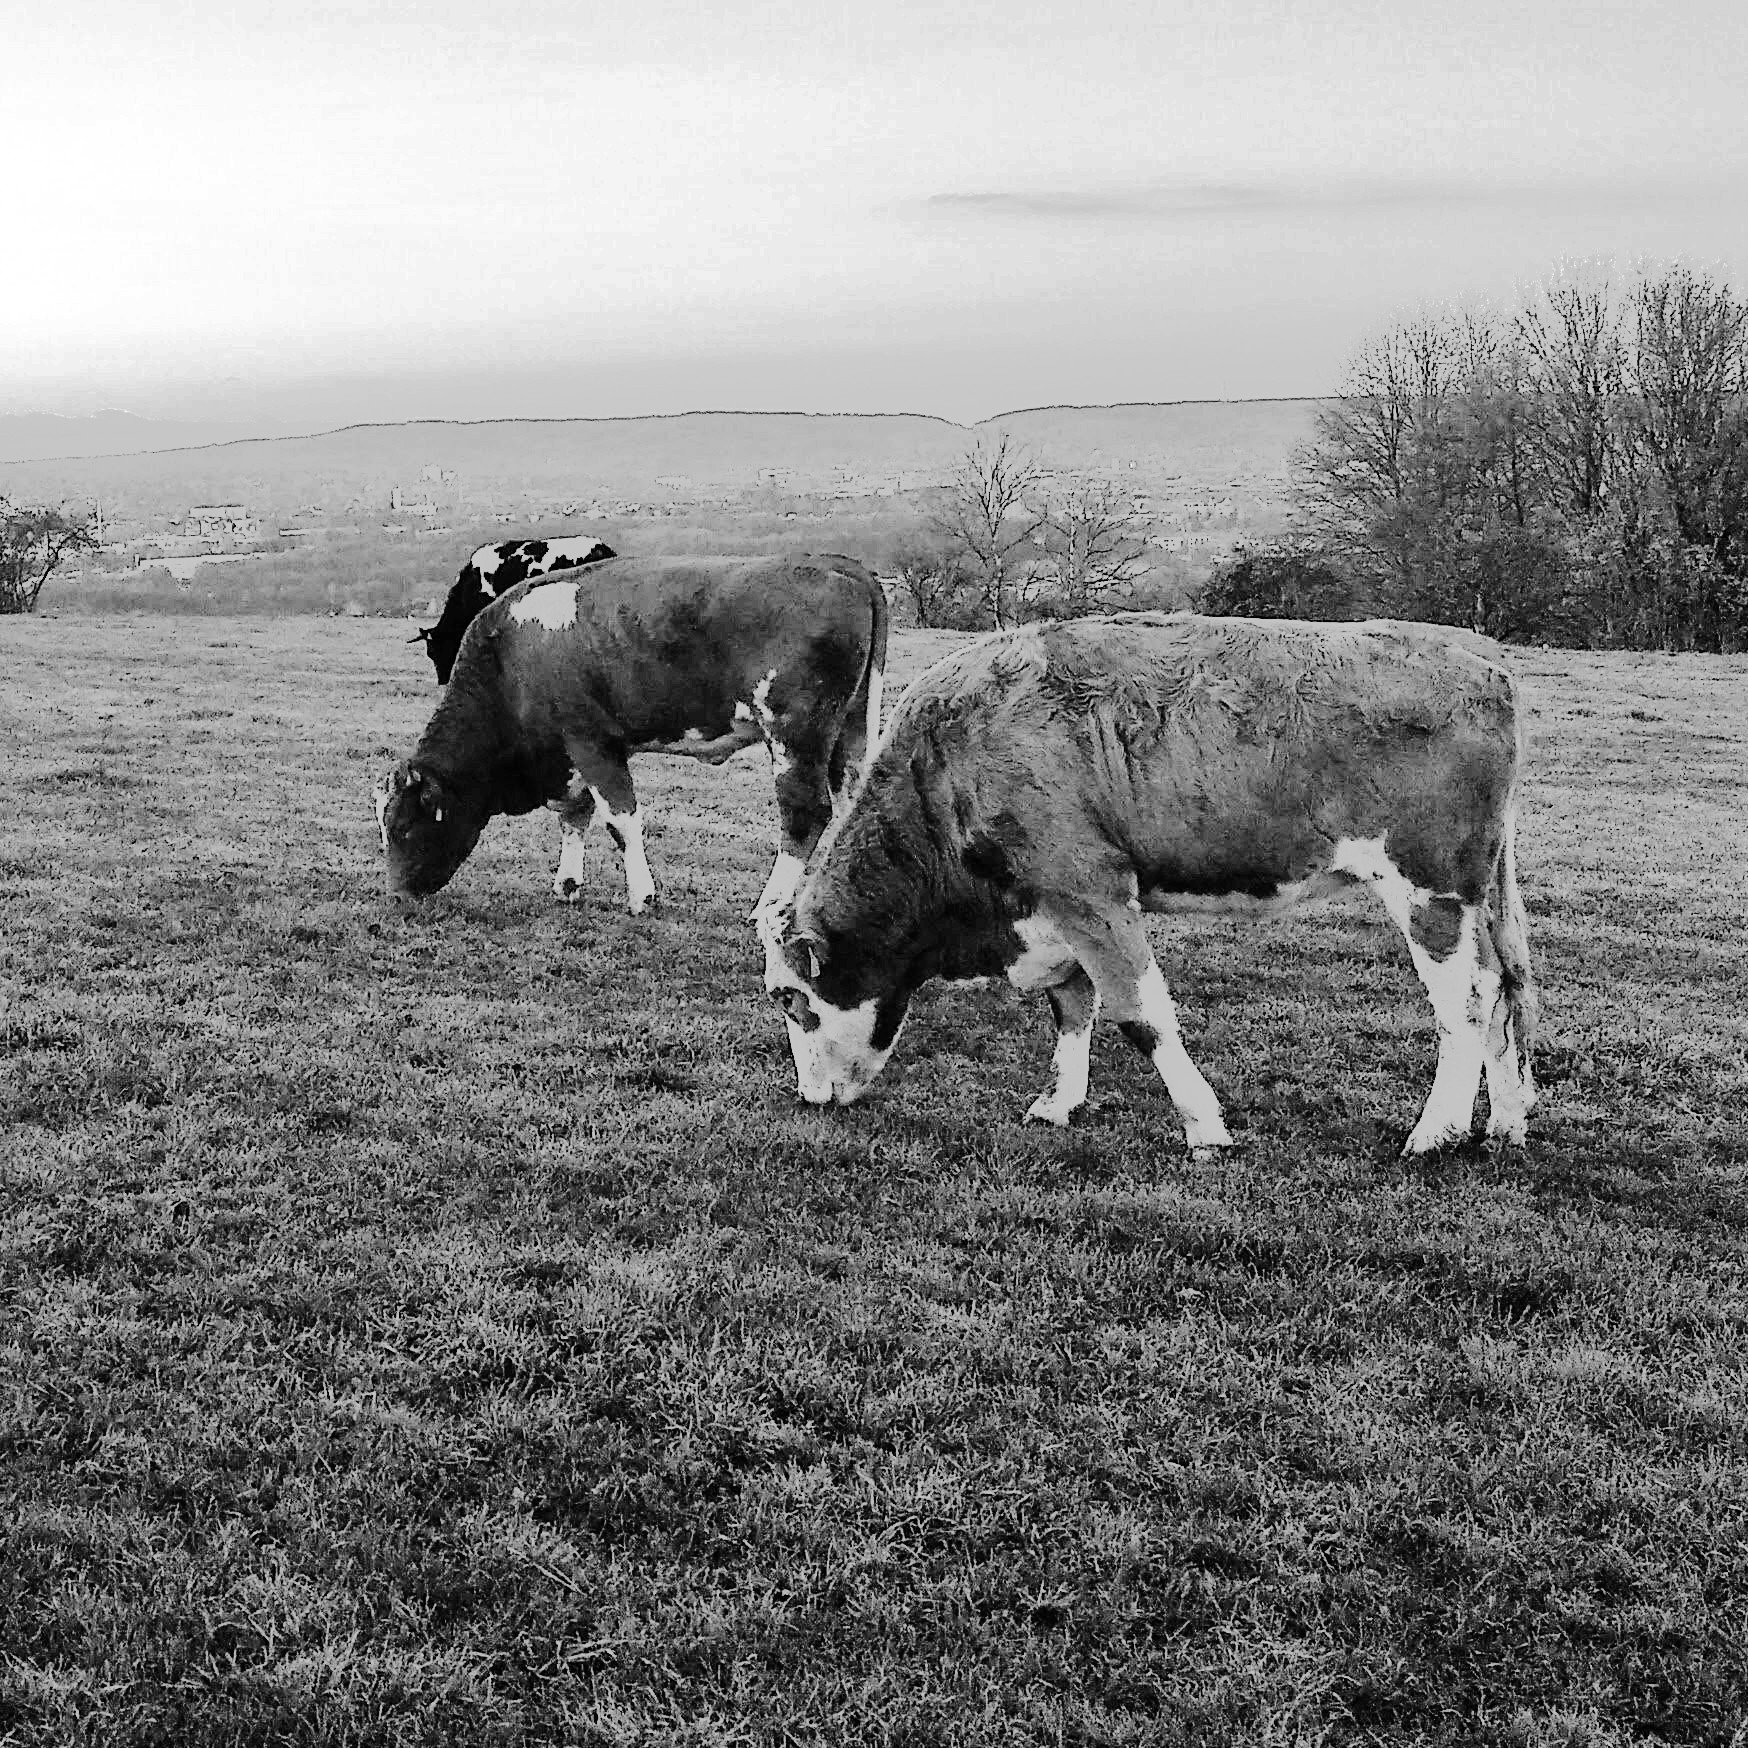
\includegraphics[
                        width=\linewidth,
                        height=\histEqImagesHeight]{equalizedCows.jpg}
                    \caption{Enhanced image}
                    \label{subFig:equalizedCows}
                \end{subfigure}
                \begin{subfigure}{0.39\linewidth}
                    \centering
                    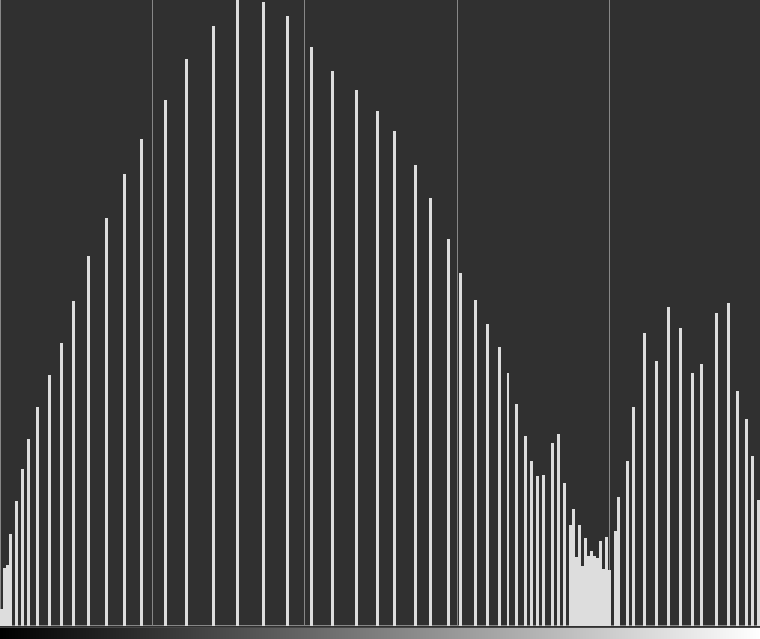
\includegraphics[
                        width=\linewidth,
                        height=\histEqImagesHeight]{equalizedCowsHist.png}
                    \caption{Equalised histogram}
                    \label{subFig:equalizedCowsHist}
                \end{subfigure}
                \caption[Example of histogram equalisation]{Example of histogram equalisation. Photo: author}
                \label{fig:histogramEqualizing}
            \end{figure}
            
            For an image of size \(M\times N \), where \(f(x,y)\) is a pixel at coordinates \(x, y\), is the image with an equalised histogram computed as follows. In the histogram \(H\), the quantity of each value from the range \(L\) is placed as follows~\cite{X3IOSjMG1S81OB7w}:
            %
            \begin{equation}
               H(i) = \sum_{x=1}^{M}\sum_{y=1}^{N}
                \begin{cases}
                    1\quad f(x,y) = i \\
                    0\quad otherwise
                \end{cases} \enspace .
            \end{equation} \label{eq::histogramCalculation}
            %
            The pixel \(g(x, y)\) in the output picture at coordinates \(x, y\) is than calculated as follows:
            %
            \begin{equation}
                g(x,y) = \frac{C\!DF(f(x,y)) - C\!DF_{min}}{M\cdot N - C\!DF_{min}} \cdot (L-1) \enspace ,
            \end{equation} \label{eq:equalizedImagePixel}
            %
            where \(CDF\) is the cumulative distribution function with minimum \(KDF_{min}\) which is defined as follows:
            %
            \begin{equation}
                CDF(j) = \sum_{i=1}^{j} H(i) \enspace .
            \end{equation} \label{eq:histogramKDF}
            %
            The explained process takes into account the global histogram for the whole image. Sometimes, such an adjustment is not sufficient and it is necessary to use a more complex method. A method created by a simple modification in this method, which gives significantly better results, is called the adaptive histogram equalisation (AHE). The adjustment is not to use the global histogram, but a local histogram created from the neighborhood around the calculated pixel. Another additional option of modification is the contrast limited adaptive histogram equalization (CLAHE), which does what AHE does, but also clips the quantities to a certain limit~\cite{X3IOSjMG1S81OB7w}.
            
        \subsection{Scaling}
            Scaling is such image processing in which the size of the image is changed.

        \subsection{Crop}
            Crop of the image is a method of removing unwanted parts of the image. By using crop the wanted part of the image stands out more.
        
    \section{Local image features}
        Local features are such a pattern that is clearly distinguishable within its closest neighborhood. Usually, the feature is some change of a property of an image, despite the fact that the feature does not have to lie directly on the change. Usually, the properties of an image are: luminance, color or texture. Different examples of features can be seen in the image~\ref{fig:localFeaturesExamples}. The features may be edges or small image patches as can be seen in the left outline drawings. Features are often points, such as points (marked with small circles) in the image on the right. The features neighborhood is usually described after the detection of the features in the image and the products of that are the descriptors of the features. The process of describing the features is then called  description or extraction of features. The descriptors are then what is usually used for various purposes~\cite{Mikolajczyk2015}.
        
        \begin{figure}
            \centering
            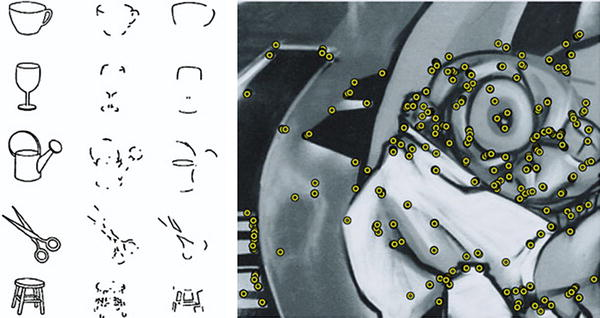
\includegraphics[width = 0.8\linewidth]{pictures/localFeaturesExamples.jpeg}
            \caption[Examples of all possible features]{Examples of all possible features. Features might be lines or surfaces as in outline drawings or points as in the grayscale image. Illustration is taken from~\cite{Mikolajczyk2015}.}
            \label{fig:localFeaturesExamples}
        \end{figure}
        
        The features are sometimes also called keypoints, or interest points. The image features are studied for a long time and the first paper was published in 1954. Feature detection has evolved a lot since then. One of the interesting properties is that the combination of features detected on straight lines and rectangular corners is often an indication of structures made by humans~\cite{Mikolajczyk2015}.

        \subsection{Categories of features}
        There can be three categories of use of algorithms that have something to do with features detection. This is not the only way to categorise these algorithms, but their categorisation in this way helps to determine which properties of features are important in which situations. The first case of use (first category) is when meanings are assigned to the features. A good example is when it is assigned the meaning of being roads or railroads to the line features in the aerial photos. In the second case of use, the features are used as anchors. Such features have to be reliably detected (all the time at the same location) among multiple detections. Good examples of such use are searching for matches, object tracking or creating panoramas. In the third category, the features are used as a representation of the content in the image. Here it is not the meaning of individual features or accurate location that is important, but rather the properties of all the features together as a whole. Categorization of the image content is a good representation of this category~\cite{Mikolajczyk2015}.
        

        
        \subsection{Local features properties}
        Local features are such features that have a specific spatial meaning in regard to their neighborhood.  Such neighborhoods may be any area in the image. As a result, the local features have reasonable invariance across unfavorable visibility conditions. Ideally, however, the features should represent some meaningful geometric objects. But this is complicated and it is not even considered nowadays. However, quality algorithms of feature detection should have the following properties (not necessarily all of them at the same time)~\cite{Mikolajczyk2015}:
        %
        \begin{description}
            \item[Repeatability] If there are  multiple photos of the same object and a feature is detected in one picture, then the feature has to be also detected in other photos (if the feature is properly visible). There are two ways to achieve repeatability. The first way is the invariance of transformations, such as rotation or scaling. The second way is the robustness, which is meant as insensitivity to noise or other minor influences. Examples of both ways and high repeatability can be seen in image~\ref{fig:localFeaturesRepeatibality}.
            \item[Distinctiveness] Feature with this property can be well distinguished from other features detected in the image or in other images. To some extent, this property is in contradiction to invariance and robustness. The invariance and robustness are usually done by ignoring some information and that leads to less information by which the feature can be distinguished.
            \item[Locality] Is the property of the feature depending only on the neighborhood of the feature.
            \item[Quantity] The number of features should be big enough to cover sufficiently even small objects in the image. In some cases the high number of features is not convenient so a limit of the features quantity has to be set.
            \item[Accuracy] If the same feature is detected in two different images, then the location has to be in the same place in relation to the spatial configuration of the two images.
            \item[Efficiency] Short computation time is preferred especially in real-time applications.
        \end{description}
        
        \begin{figure}
            \centering
            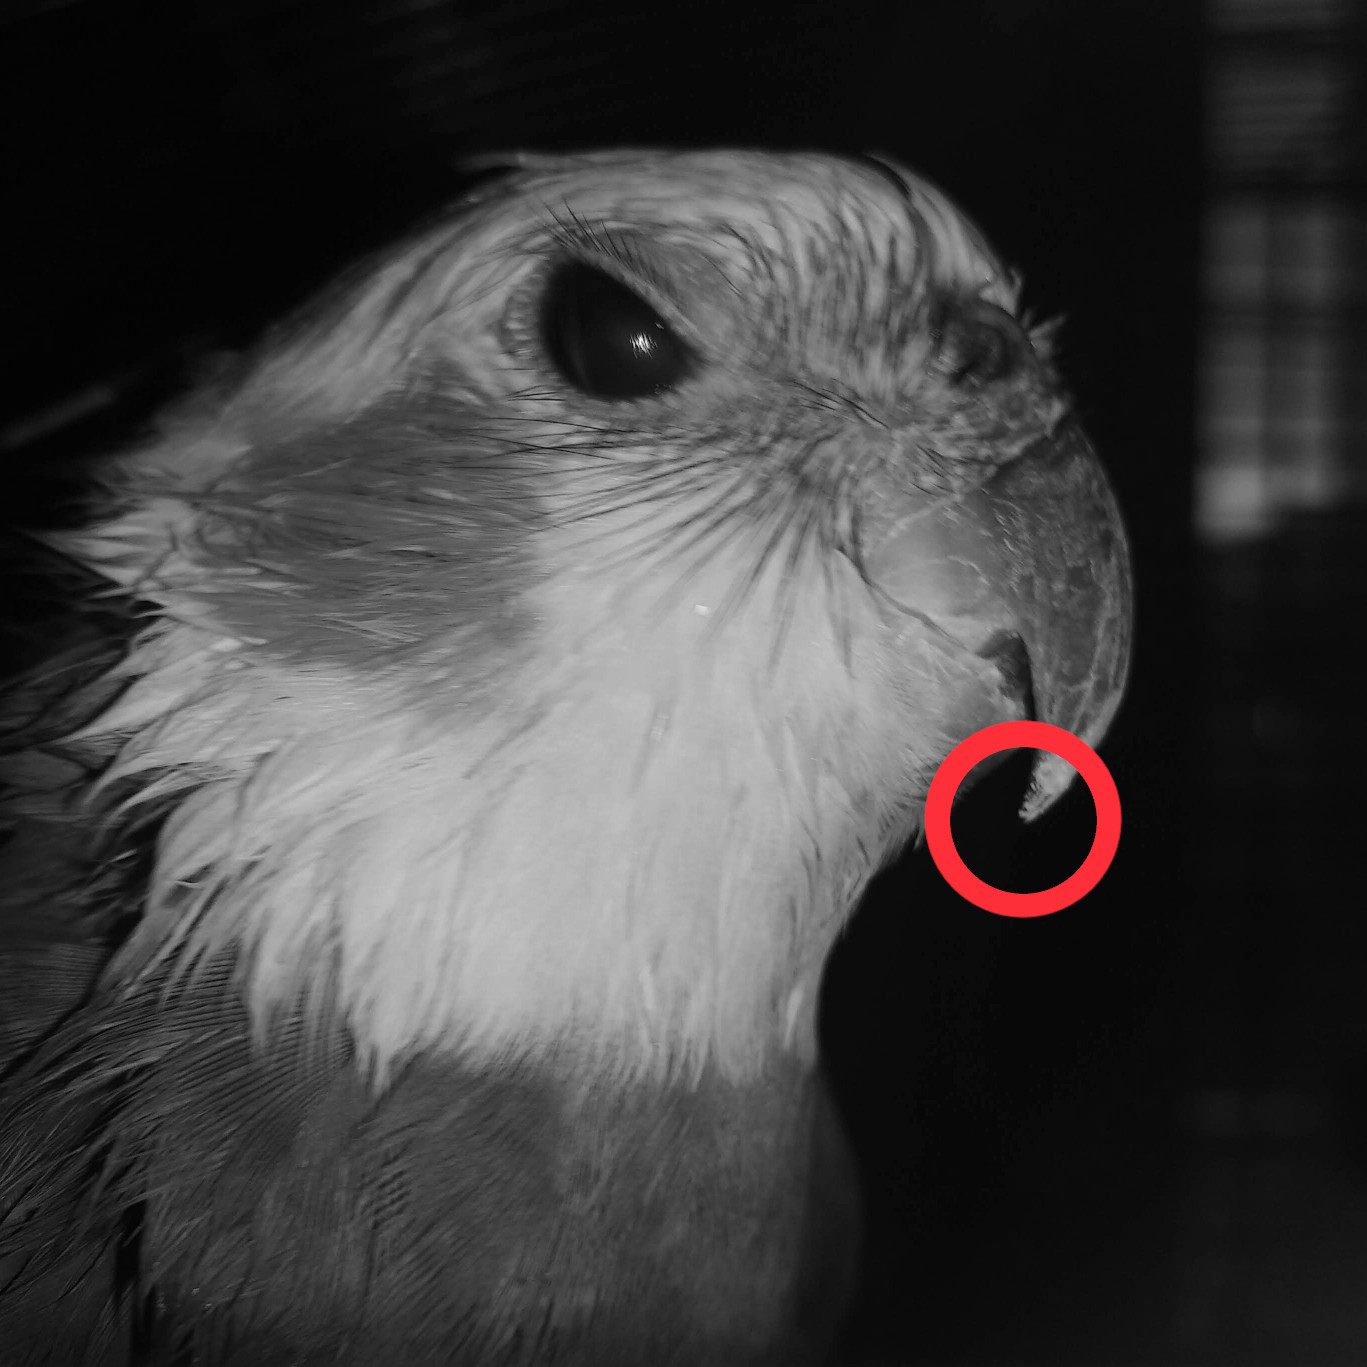
\includegraphics[width = 0.24\linewidth]{pictures/featureReference.jpg}
            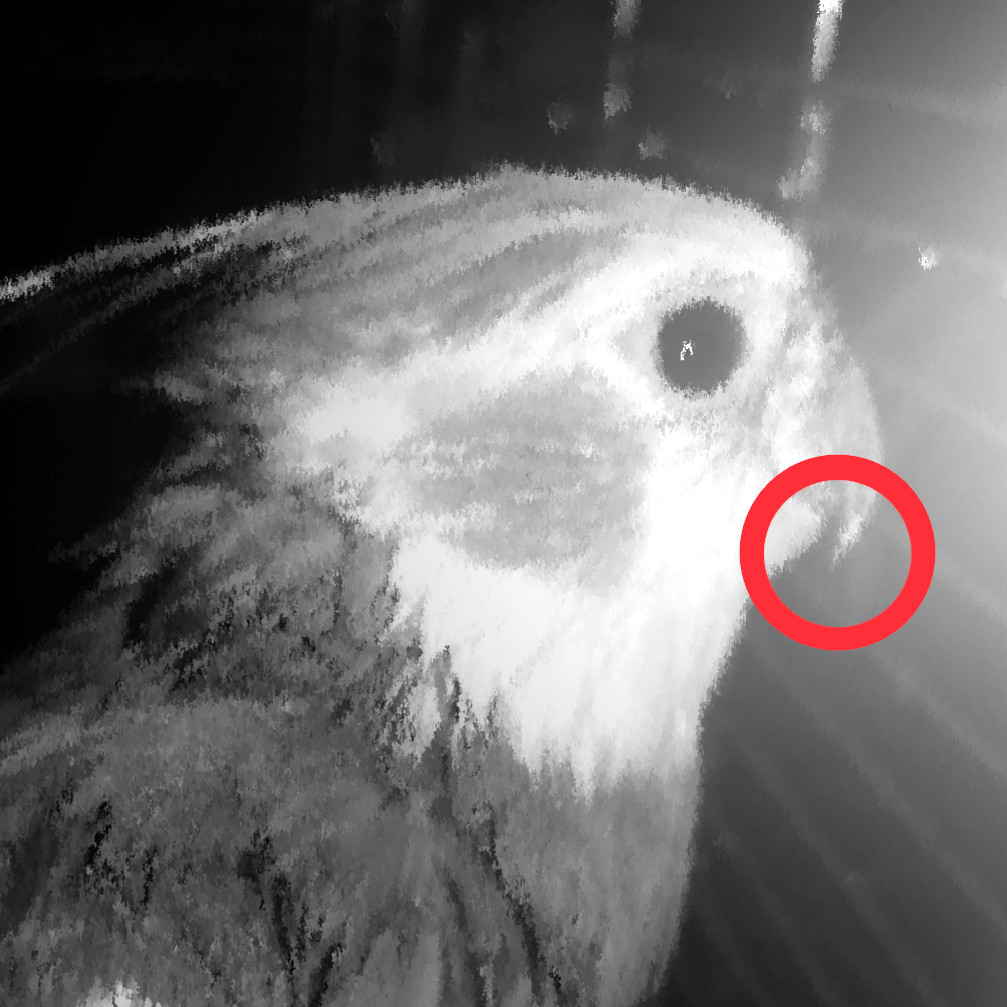
\includegraphics[width = 0.24\linewidth]{pictures/featureRobustness.jpg}
            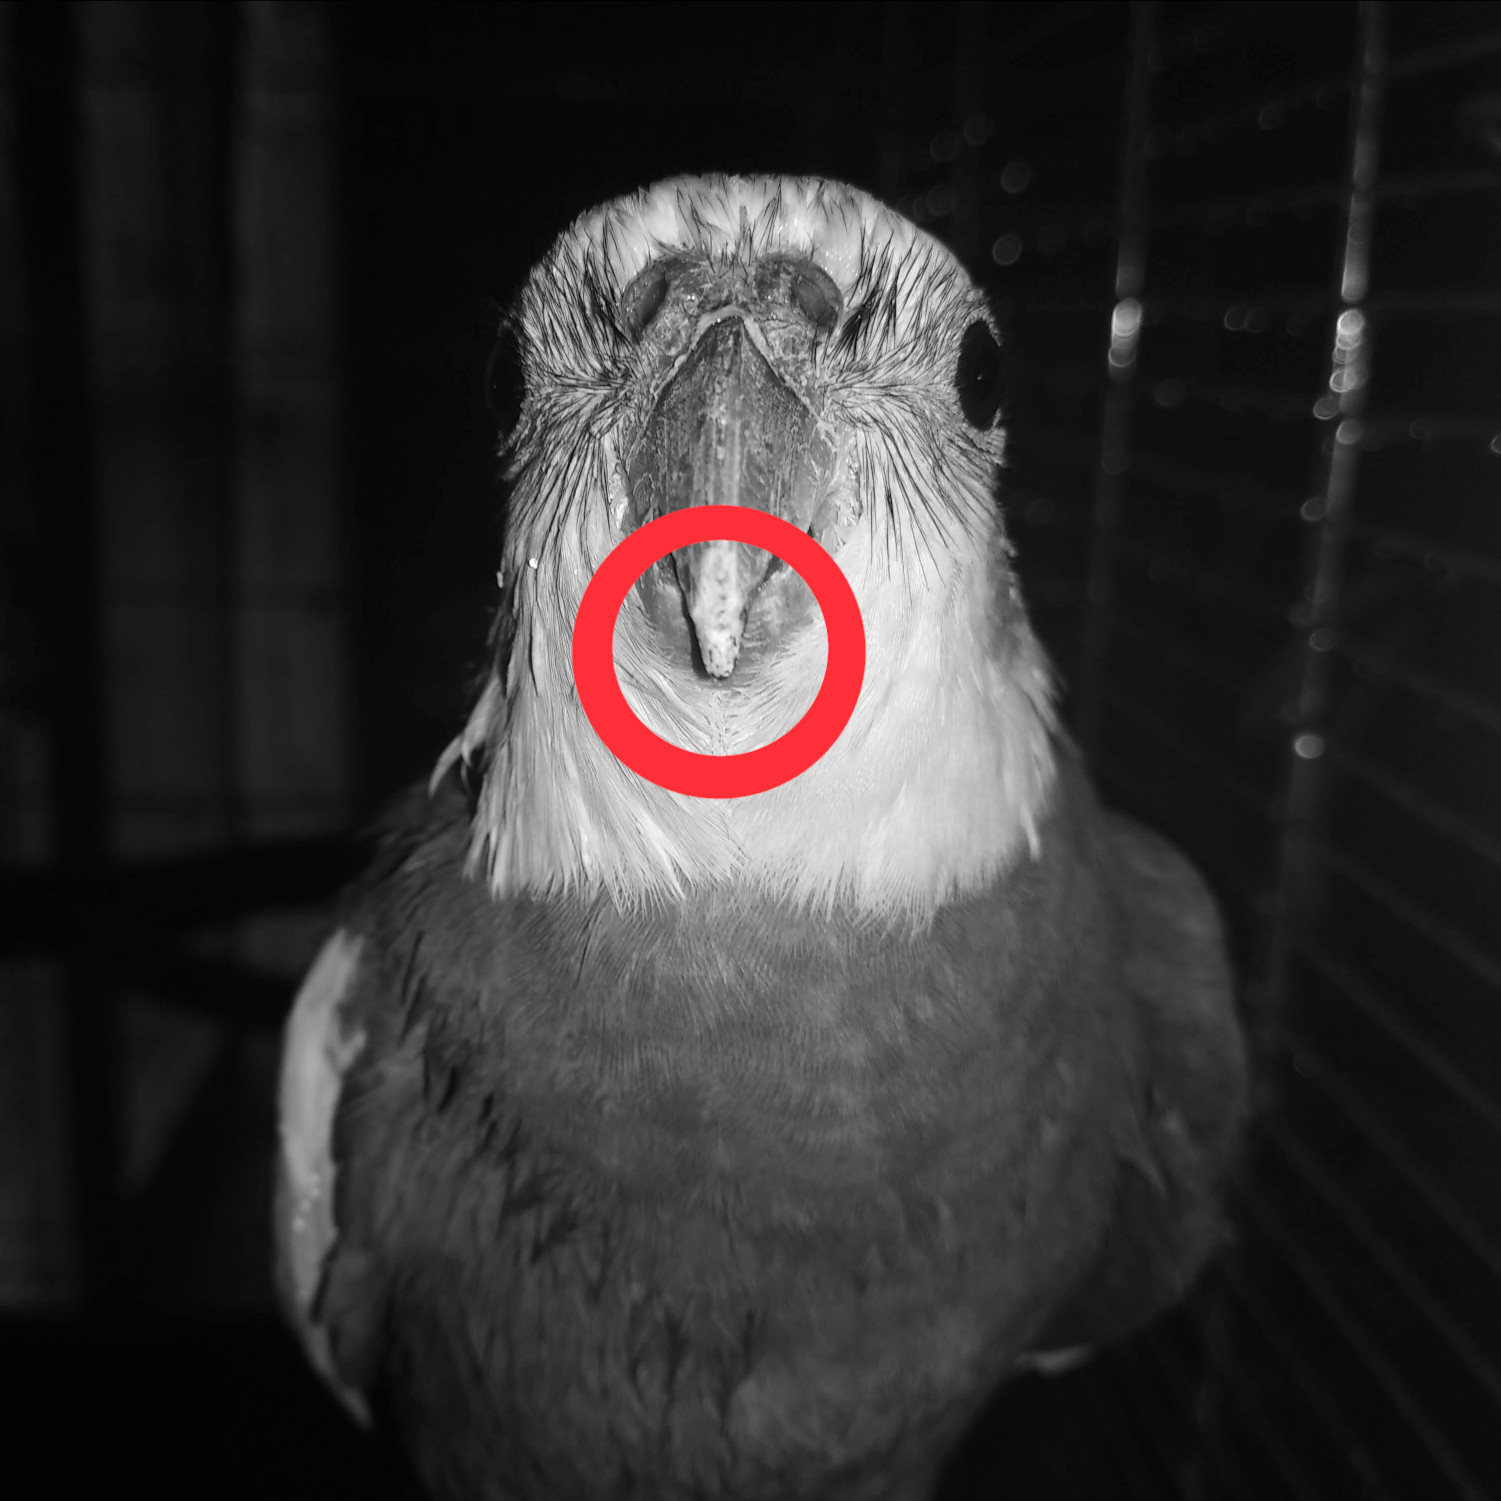
\includegraphics[width = 0.24\linewidth]{pictures/featureRotation.jpg}            \caption[Demonstration of a feature with good repeatability]{Demonstration of a feature (highlighted with the circle) with good repeatability. Feature is detected despite different angles of view, noise and slight rotation. Photo: author}
            \label{fig:localFeaturesRepeatibality}
        \end{figure}
    
    \section{Feature detection and description}
        In our thesis, several feature detection and description methods are briefly described. A more detailed description of some of these and other methods can be found in the previous bachelor thesis~\cite{Sefcik2020}.
        
        \subsection{LBP}
            Local binary patterns (LBP) are features that are calculated for each pixel in the image as follows~\cite{5427137}:
            %
            \begin{equation}
                LBP_{P,R} = \sum_{p=0}^{P-1} s\left(g_p - g_c\right) 2^p\quad where\ s(x) =
                \begin{cases}
                    1\quad x \leq 0\\
                    0\quad x > 0
                \end{cases} \enspace ,
            \end{equation} \label{eq:LBP}
            %
            \(g_p\) means an adjacent point (the point has the value of the pixel on which it is) value with index \(p\), \(g_c\) is the value of the evaluated pixel (central point). The adjacent points lie evenly on a circle around the central point. Parameters \(P\) and \(R\) determine the number of adjacent points and the radius \(R\) (measured in pixels) of the circle. For \(R=1\) the adjacent points lie in the direct neighborhood pixels of the evaluated pixel.
            
            A partial rotation invariance can be created by applying a bit shift to the right on all the calculated values. The right shift is applied until 1 is in the least significant position. With the help of this modification, the LBP is invariant to rotations of multiples of the value \(360/P\).
            
        \subsection{SIFT}
            Scale-invariant feature transform (SIFT) was patented by University of British Columbia~\cite{lowe2004method} and published by David Lowe~\cite{lowe1999object}. The patent expired in the year 2020.
        
            Further description of the SIFT is freely taken from work~\cite{5734842}. SIFT is invariant to lighting changes, orientation, uniform scaling and partially invariant to affine transformations. These properties guarantee robustness preventing many negative influences. Although it is an old method, it has good results compared to other methods according to this comparison study~\cite{1498756}.
                            
            The output of the SIFT algorithm is a list of \(N\) keypoints. The way of computing the keypoints are the following steps:
            %
            \begin{itemize}
                \item Creation of images in many different scales created from the original image. This process is often called a creation of an image pyramid. The levels of this pyramid are the images in different scales,
                \item Detecting extremes across all the images from the pyramid. The detected points are candidates of being keypoints,
                \item Keypoints localisation,
                \item The canonical rotation is assigned to these keypoints,
                \item Generation of descriptors of these keypoints.
            \end{itemize}
            %
            The output structure of keypoints \(x_i\) is defined as follows \(x_i = \{x,y,\sigma,o,f\}\), where \(x\) and \(y\) are the coordinates of the keypoint in the image, \(\sigma\) is the scale in which the keypoint was calculated, \(o\) is the canonical orientation, \(f\) is the SIFT descriptor. The descriptor is a vector of 128 floating point numbers.
        \subsubsection*{RootSIFT}
            RootSIFT is a modification of the SIFT algorithm that increases the accuracy without greater memory storage requirements or significantly higher processing cost~\cite{arandjelovic2012three}. The modification of the algorithm is not complicated and it consists of a few steps after the keypoints description. The steps are as follows:
            %
            \begin{description}
                \item[First step] The first step is to L1 normalise the SIFT descriptors (originally they are L2 normalised).
                \item[Second step] Square root all the descriptors
                \item[Third step] L2 Normalise all the descriptors.
            \end{description}
            %
            L1-normalised vectors must meet following condition:
            %
            \begin{equation}
                \sum_{i=0}^{n} x_i = 1 \ and  \ x_i \geq 0 .
            \end{equation}
            %
            L2-normalised vectors must meet following condition:
            \begin{equation}
                \sum_{i=0}^{n} \sqrt{x_i^2} = 1.
            \end{equation}
            Descriptors in this way are then called as RootSIFT descriptors, and comparing them the same as SIFT descriptors leads to comparing them effectively by the Hellinger kernel. According to the original work that leads to an improved accuracy. The Hellinger kernel for two L1-normalised histograms(vectors) is defined as follows:
            %
            \begin{equation}
                H(x, y) = \sum_{i=0}^{n} \sqrt{x_i y_i}.
            \end{equation}
            %
            Resulting number is a coefficient that can be used for the comparison.
                
        \subsection{BEBLID}
            Boosted efficient binary local image descriptor (BEBLID) is a feature descriptive method that is a binary modification of Boosted efficient local image descriptor BELID (based on real values)~\cite{SUAREZ2020_paper}. According to the experiments in the study, where the BEBLID was introduced~\cite{SUAREZ2020_paper}, it beats the accuracy and speed of other top performing descriptors ORB, BinBoost and LATCH at the time (BEBLID was published in 2020).  
            
            The feature detection works on comparing pairs that are created from the learned sampling patterns. Sampling patterns are predetermined pairs of points to be compared around the place that is going to be described. There is also a process that creates the descriptors invariant to Euclidean transformations.
            
            In the whole process, a term weak learner is used, which means a function that creates responses to an image patch around a feature. The responses are marked \(h(x)\) and they create a vector of \(K\) learning responses to the weak learner and \(h_k(z) \equiv h_k(x; f, T)\) is called the k-th weak learner. The weak learner depends on the feature extraction function \(f\) and threshold \(T\) and the \(h_k(x)\) is defined as follows:
            %
            \begin{equation}
                h(x; f, T) =
                \begin{cases}
                    1\quad if \quad f(x) \leq T\\
                    -1\quad if \quad f(x) > T
                \end{cases}.
            \end{equation}
            %
            This weak learner is defined for the BELID algorithm and to modify it to make it create binary outputs, -1 has to be mapped to 0. The feature extraction function is based on comparing pairs of mean grey values of areas around pixels. These pairs are determined by the sampling patterns. The descriptor BEBLID is then vector created by the weak learner, as seen in the figure from the original study~\ref{fig:BEBLID_explanation}
            
            \begin{figure}
                \centering
                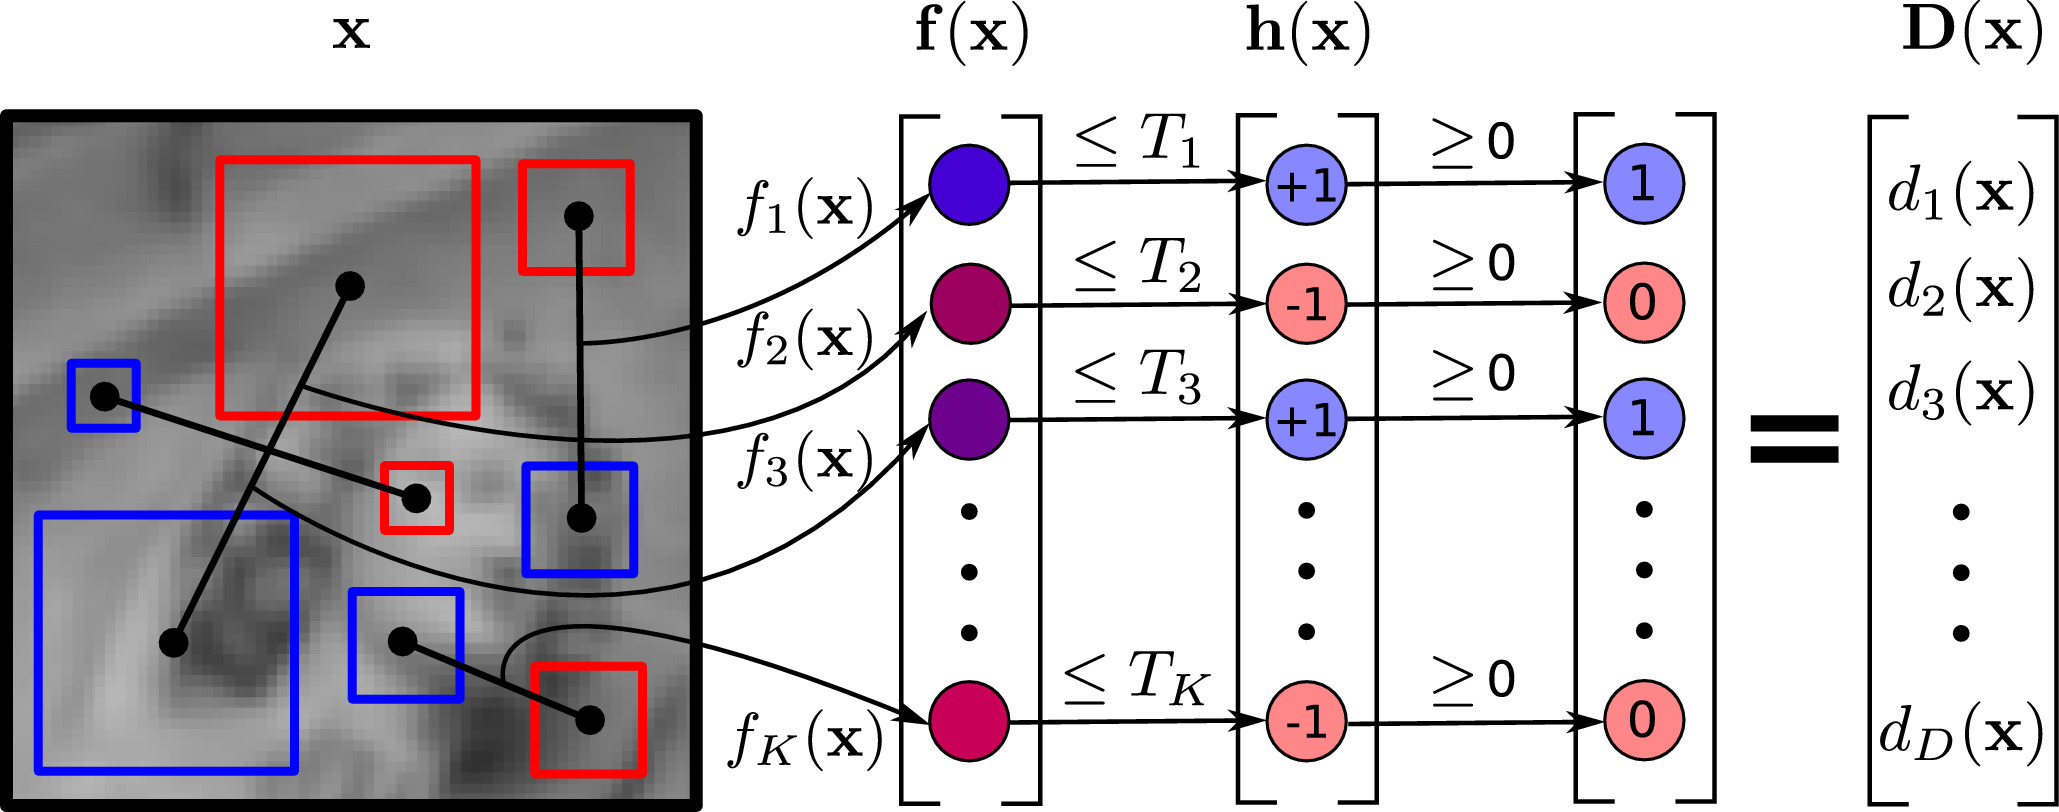
\includegraphics[width = 0.8\linewidth] {pictures/features_and_descriptors/BEBLID_explanation.jpg}
                \caption[Illustration of creating the BEBLID descriptor]{Illustration of creating the BEBLID descriptor for image patch \(x\) around detected feature. The image was taken from the BEBLID paper~\cite{SUAREZ2020_paper}.}
                \label{fig:BEBLID_explanation}
            \end{figure}
            
    \section{Feature matching}
        Feature matching is usually a process of finding the best matches for features from the reference set of features in the second set of features. Not only one best match has to be searched, some processing needs more than only the best match. Sometimes it is necessary to have \(k\) the best matches (sorted according to their similarity with the reference feature). The output of this process is a set of best matches from the second set of features for each feature from the reference set of features. Descriptors are usually used for the matching, rather than the keypoints themselves~\cite{Szeliski2010-ab}. Illustration of such a process can be seen in the image~\ref{fig:featuresMatching}.
        
        If the scenario in the image~\ref{fig:featuresMatching} compares the content of both images, then the result will probably be that similar content was found in both images. Filters can be applied to  the output matches in order to reduce the number of miss matched features (as the red match in the picture~\ref{fig:featuresMatching}). More on that topic can be found in the previous work~\cite{Sefcik2020}.
        
        \begin{figure}
            \centering
            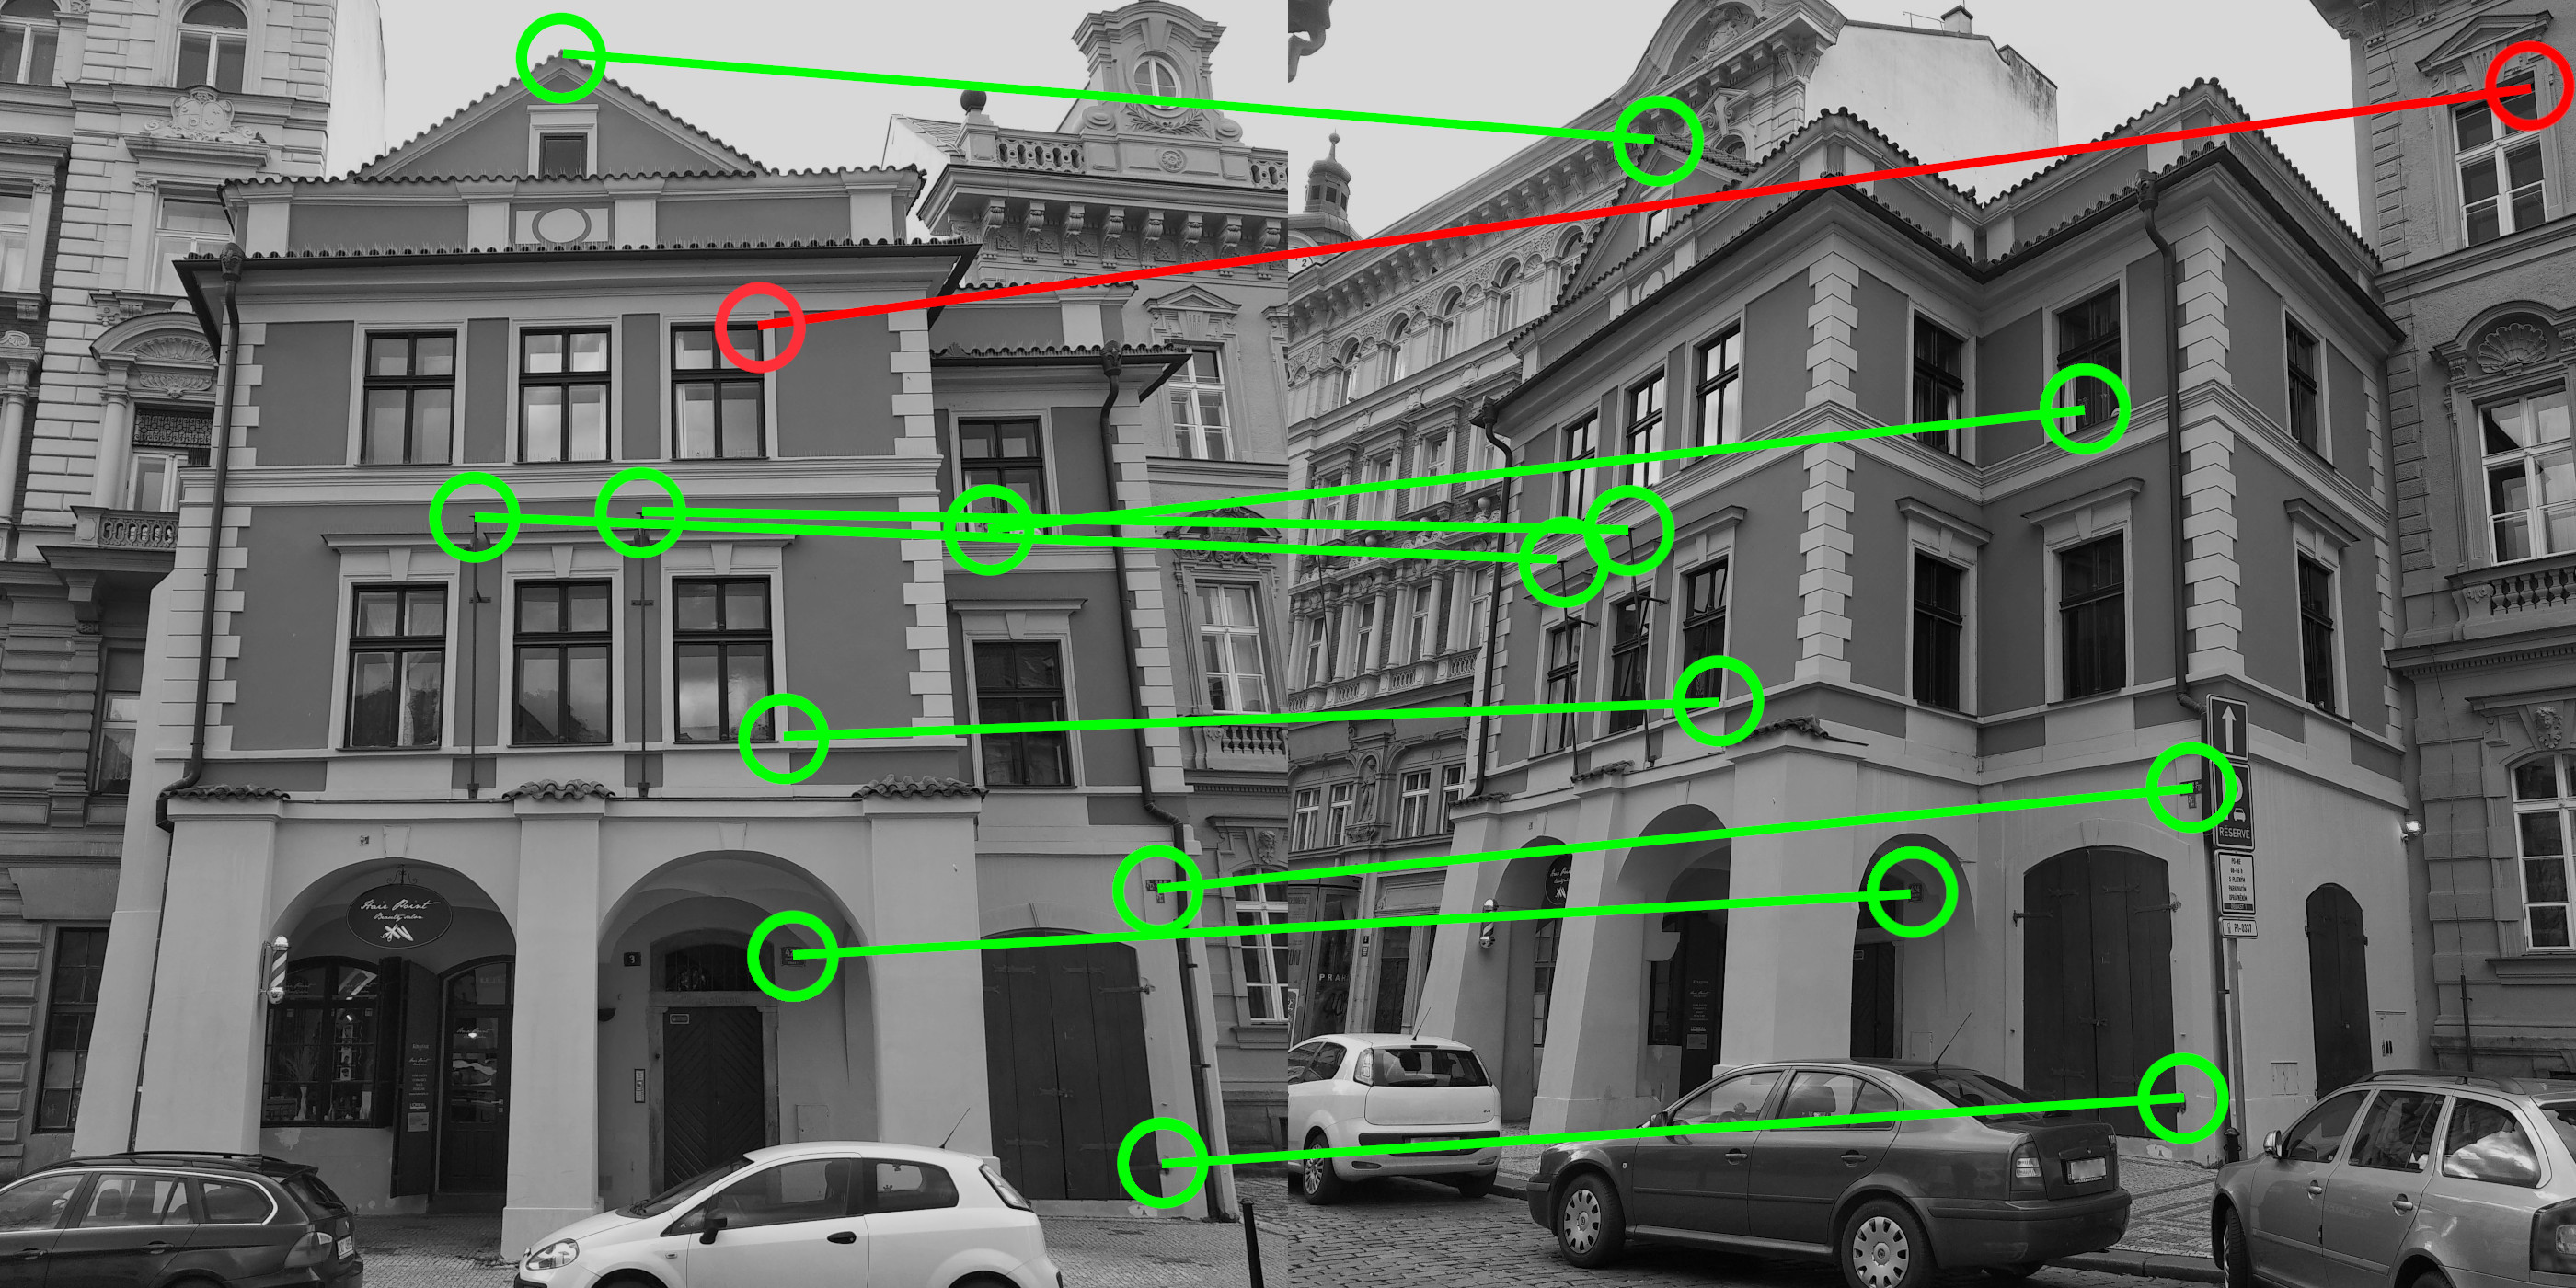
\includegraphics[width = 0.8\linewidth]{pictures/featuresMatching.jpg}
            \caption[Illustration of feature matching]{Illustration of feature matching between two images of the same building taken from different angles. The green ones are matched correctly and the red one is not correct. Photo: author}
            \label{fig:featuresMatching}
        \end{figure}

        \subsection{Methods of feature matching}
            A match for two features is such a pair in which the features are the most similar ones from two sets of features. The Euclidean distance is used in comparing the SIFT features~\cite{1315206}. For binary-based descriptors (like ORB), the Hamming distance is usually used~\cite{Mordvintsevc2013}. The smaller the distance, the more features are considered to be similar. Features with zero distance are then considered identical~\cite{1315206}.
                
            \subsubsection*{Brute force matching}
                Straightforward and simple way of feature matching is to use brute force. When using this method, each feature from the first set of features is compared to each feature from the second such set~\cite{Mordvintsevc2013}. Because the time complexity is quadratic, time increases rapidly with the number of features.
                
            \subsubsection*{FLANN based matching}
                For faster matching of large sets of features, a method based on a freely accessible library called Fast Library for Approximate Nearest Neighbors (FLANN) is usually used. With this method, the match is found with the use of hierarchical structures (randomized kd-trees, hierarchical k mean trees or hierarchical clustering algorithm for ORB). It is important to note that for some structures the search does not guarantee the best match. It produces an approximation of the best match~\cite{6233169}.
                
        \subsection{Methods of filtering matches}
            As mentioned above, some features might be miss matched. In this section it is explained how it is possible to try to remove these mismatches.

            %cross check
            \subsubsection*{Cross-check Test}
                    A filter with a simple but working approach is the Cross-check Test. The idea is to match the features in two directions. First, searching the best matches for features from the first set of features in the second set, and then doing the same in the opposite direction. Only the matches that have been found in both directions are not filtered out~\cite{Mordvintsevc2013}.
                
            %loweho poměrový test
            \subsubsection*{Lowe's ratio test}
                Another method of filtering matched features is the Lowe's ratio test. This method introduced in the study~\cite{lowe2004distinctive} filters the matches based on the ratio the closest match distance to the second closest match distance. For this filter, it is necessary that at least two found matches per feature. If the ratio of distances \(\frac{best\enspace match}{second\enspace best\enspace match}\) is greater than some threshold, the match is filtered out. This filter guarantees that the match is the best by large margin, so there is not any similar possible match. Lowe states in his study that the threshold should be set between 0.7 to 0.8, as can be seen in the image~\ref{fig:lowesRatioTest}. There is a graph of multiple tests of this filter and its results.
                
                \begin{figure}
                    \centering
                    \begin{tikzpicture}
                        \begin{axis}
                        [xlabel={Distance ratio (closest one to second closest one)},ylabel={DF}, grid=both,
                        ymin=-0.01,ymax=0.75, width = 0.7\linewidth, legend pos=north west]
                            \addplot[blue] table{./data/loweRatioTestGoodMatches.txt};
                            \addlegendentry{DF for correctly matched matches}
                            \addplot[red] table{./data/loweRatioTestBadMatches.txt};
                            \addlegendentry{DF for miss matched matches}
                        \end{axis}
                    \end{tikzpicture}
                    \caption[Probability density function (DF) of correct and bad matches]{Illustration of probability density function (DF) of correct and bad matches depending on the ratio measured by D. Lowe in the study~\cite{lowe2004distinctive}.}
                    \label{fig:lowesRatioTest}
                \end{figure}
                
                %RANSAC
            \subsubsection*{RANSAC}
                Random Sample Consensus (RANSAC) is a method used for interpreting and smoothing data containing a large number of gross errors. It is important to note that this is not a filtering method, but it rather just extracts the correct interpretation of the data as a whole. This method is often used in computer vision because the feature detection algorithms are prone to errors~\cite{Fischler1981}.
                %TODO make bigger description
                
    \section{Perspective-n-Point problem} \label{sec:rotTransMat}
        Perspective-n-Point problem (usually referred only as PnP problem) is about finding the correct transformation of points from world space to local camera space when specific information is known. The information must contain the geometry of the points in world space (3D coordinates) and where they have been projected in the image taken by the camera (2D coordinates). The focal length of a camera, the sensor size, and the resolution has to be known as well~\cite{Riba2021}.
        
        An illustration of the problem can be seen in the image~\ref{fig:pnpProblem}. Where \(c_i\) are 3D points in world space, \(u_i\) are their projections, the translation matrix \(t \in \mathbb{R}^{3,1}\) and rotation matrix \(R \in \mathbb{R}^{3,3}\) create together the resulting transformation~\cite{Riba2021}.
        
        \begin{figure}
            \centering
            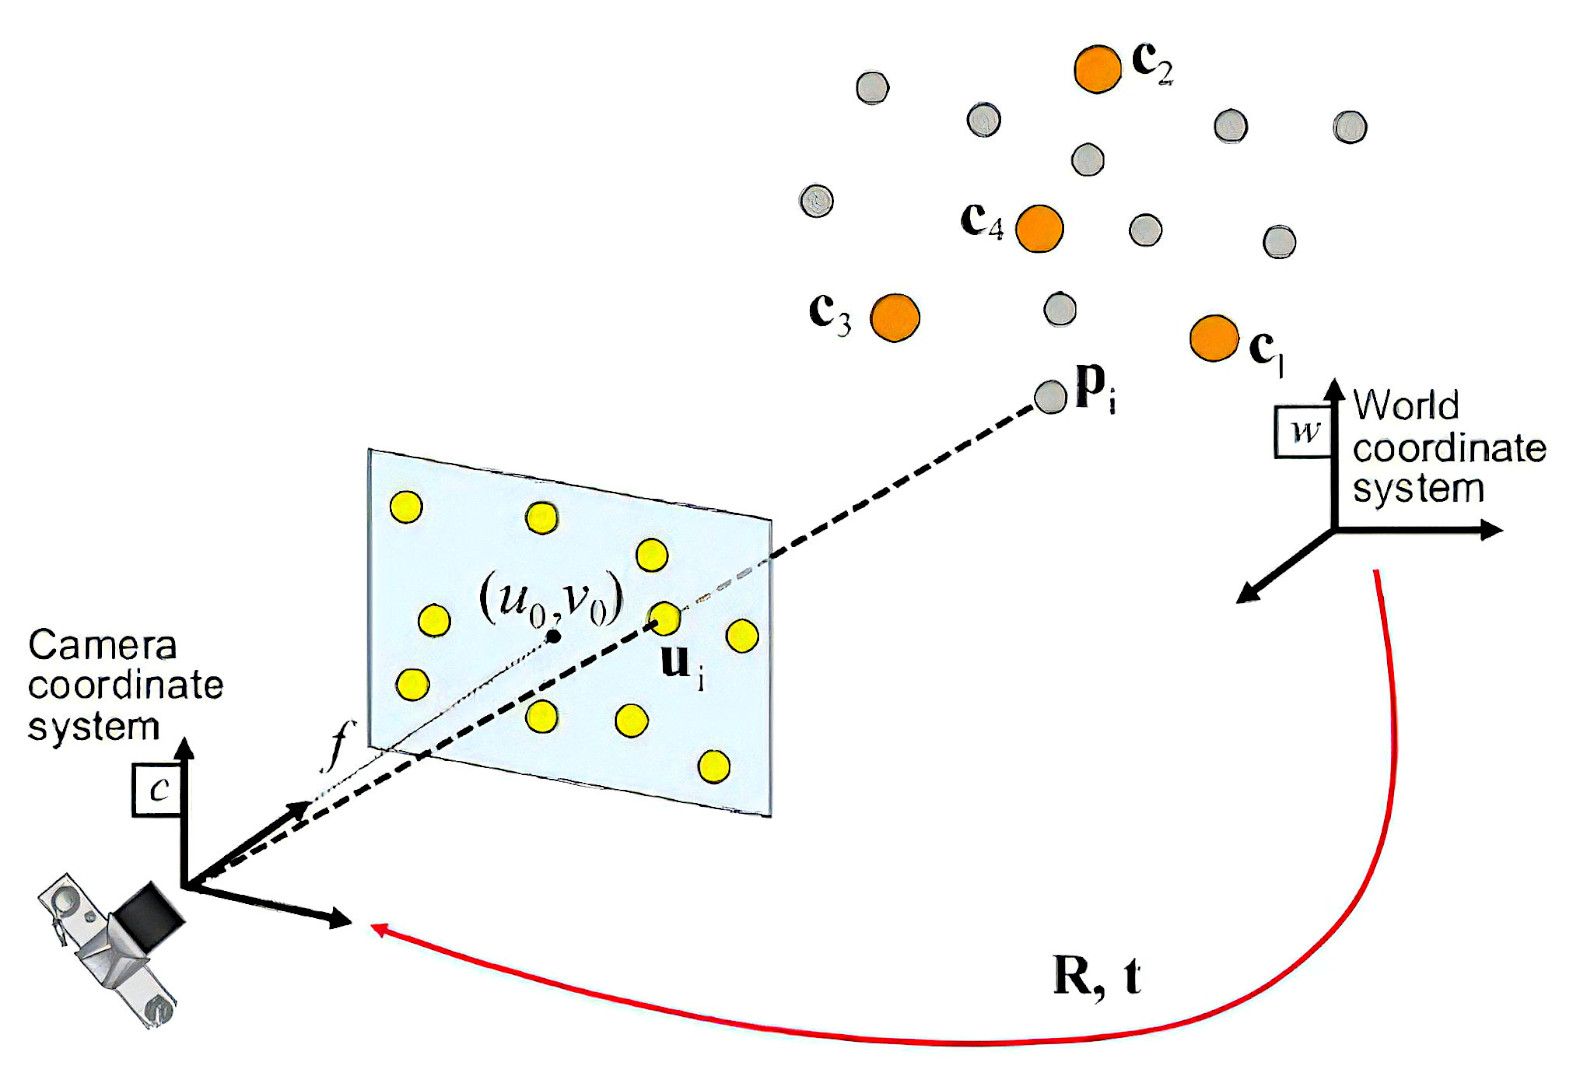
\includegraphics[width = 0.9\linewidth]{pictures/research/pnp_small.jpg}
            \caption[Illustration of the Perspective-n-Point problem]{Illustration of the Perspective-n-Point problem. Image was taken from OpenCV tutorial~\cite{Riba2021}.}
            \label{fig:pnpProblem}
        \end{figure}   
        
        To project the 3D points into the image, the transformation has to be used with the projection matrix \(A\) in the following way:
        \begin{equation}
            s
            \begin{bmatrix}
                u \\
                v \\
                1
            \end{bmatrix}
            =
            A
            \begin{bmatrix}
                1 & 0 & 0 & 0\\
                0 & 1 & 0 & 0\\
                0 & 0 & 1 & 0
            \end{bmatrix}
            \begin{bmatrix}
                r_{1, 1} & r_{1, 2} & r_{1, 3} & t_1\\
                r_{2, 1} & r_{2, 2} & r_{1, 3} & t_2\\
                r_{3, 1} & r_{3, 2} & r_{3, 3} & t_3\\
                0 & 0 & 0 & 1           
            \end{bmatrix}
            \begin{bmatrix}
                x\\
                y\\
                z\\
                1\\
            \end{bmatrix}.
        \end{equation}
        %
        The final step is to divide the resulting vector by the \(s \in \mathbb{R}\). The matrix \(A\) can be created from the information about the camera as follows:
                \begin{equation}
                   A =  \begin{bmatrix}
                            f_x & 0 & c_x\\
                            0 &   f_y & c_y \\
                            0 &  0    & 1
                        \end{bmatrix}, \enspace
                        c_x = \frac{w}{2}, \enspace
                        c_y = \frac{h}{2}, \enspace
                        f_x = \frac{w \cdot f}{s_x}, \enspace
                        f_y = \frac{h \cdot f}{s_y}, \enspace
                \end{equation}
                where \(w\) is a width, \(h\) is a height of the image resolution, \(s_x\) is a size of the camera sensor in horizontal direction, \(s_y\) is then a size in vertical direction and \(f\) is the focal length of the camera~\cite{Riba2021}.
            
\chapter{The context of our work}
    This chapter describes the context of our thesis within the \textit{Dowry Towns of Bohemian Queens} project (further called also as DTBQ). Many theses were created within this project. Two of these and the project itself are introduced in this chapter.
    
    %TODO if having some time add some information about Štěpán's thesis or possibly also Slabý's thesis
    \section{The Dowry Towns of Bohemian Queens project}
        This project was named after a group of towns that were owned by Czech queens in the past. The institution of the towns owned by Czech queens was established at the beginning of the 14th century and ceased to exist in 1918. In group of these towns belong Hradec Králové, Chrudim, Vysoké Mýto, Polička, Jaroměř, Dvůr Králové, Trutnov, Nový Bydžov and Mělník. As can be seen in the map~\ref{img:vennaMestaMapa}, the towns except Mělník are located in the east of Bohemia~\cite{ghLr7y27wY4pk4xP}.
        
        \begin{figure}
            \centering
            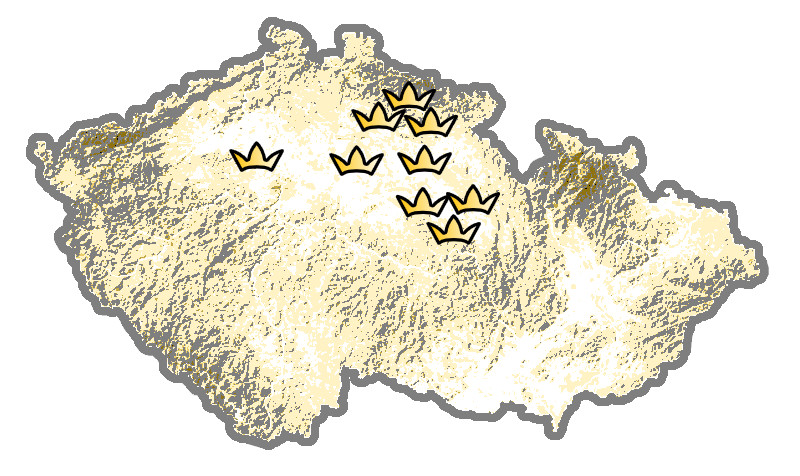
\includegraphics[width = 0.6\linewidth]{pictures/kontextPrace/vennaMesta.jpg}
            \caption[Location of dowry towns in the Czech Republic]{Location of dowry towns in the Czech Republic. Image is taken from website of the DTBQ project~\cite{ghLr7y27wY4pk4xP}.}
            \label{img:vennaMestaMapa}
        \end{figure}
        
        \subsection{History of the dowry towns}
        Several queens had their court in Mělník. One of them was Queen Barbora Celská, the wife of King Zikmund Lucemburský, or Queen Johana z Rožmitálu, the wife of King Jiří z Poděbrad. Hradec Králové was a favorite town of Queen Alžběta Rejčka, the first queen to have dowry towns. She got the towns when her husband Václav~\RN{2} registered her 20~000~hryvnias of silver on the selected East Bohemian towns before his death. Hradec Králové was also a favourite town of Queen Alžběta Pomořanská, the wife of King Karel~\RN{4}. However, she was very unpopular in the town because she created big debts on the account of the town. Thanks to this rich history, the dowry towns are strongly connected to the Czech history and until nowadays they are considered to be part of the Czech regional identity~\cite{ghLr7y27wY4pk4xP}.
        
        \subsection{Project goals}
        The goal and content of the project is to study the presentation of dowry towns with the help of modern technologies of computer graphics and tools of historical geography. The main outputs of the project will be mobile application and a website that is planned to be used as a historic guide for the dowry towns. On the website, users will be guided through the urban landscape of dowry towns using specialised maps of the entire region or each town. A 3D reconstruction of buildings, which stood or still stands, for Hradec Králové will be created and offered to the users in virtual reality with examples from the life of people in the past. Set of products will be published to the public to help to inform about dowry towns and popularize the history of these towns~\cite{ghLr7y27wY4pk4xP}.
    
    \section{Urban scene recognition and editing}
        The \textit{Urban scene recognition and editing} thesis, on which this one continues, is written by Jan Šefčík~\cite{Sefcik2020}. Within the DTBQ project, this work deals with technical problems in the field of smartphone application, especially with the problem of localisation based on computer vision. Based on this, building images can be displayed in the scene of smartphone cameras.
        
        Main goals of the thesis are established as follows:
        %
        \begin{itemize}
            \item Researching the possibilities of urban scene recognition,
            \item Analyse the found possibilities and their restrictions within the DTBQ project,
            \item Design and realisation of a prototype that determines the location using the geolocation and image data,
            \item Testing the realised prototype and comparing it to the limitations within the DTBQ project.
        \end{itemize}
        %
        The first two goals, researching and analysing methods of image pre-processing, feature detection and extraction, and feature matching and filtering are met in the theoretical part of the thesis. Their suitability within the DTBQ project is discussed too and in the chapter of analysis, there are some useful notes for improvements.

        \subsection{Design of Šefčík's work}
        The practical part of Šefčík’s thesis is devoted to a mobile application design and a realisation. Application properties and functional and non-functional requirements are specified within the design.

        The requirements can be simplified as follows:
        %
        %TODO if still have time, ZLEPSIT, protoze mam obor SI tak by se melo toto vice rozvést
        \begin{description}
            \item[Functional requirements:] The application runs in real-time, weather adaptation, accuracy of the localisation, easy administration of the database of the historical objects, saving data in the application.
            \item[Non-functional requirements:] The application runs on the Android operating system version 9.0 and higher, modularity, quality documentation in the form of technical documentation and documentation for programmers, user manual and video manuals for administrators.
        \end{description}
        
        \subsection{Realisation and testing in Šefčík's thesis}
        The design included a much wider area than the realisation itself. The state of finished implementation is well illustrated by the activity diagram in the image~\ref{img:sefcikDiagramAktivit}. The realised implementation is therefore a prototype of the image recognition and localisation of the object in an image.
        
        \begin{figure}
            \centering
            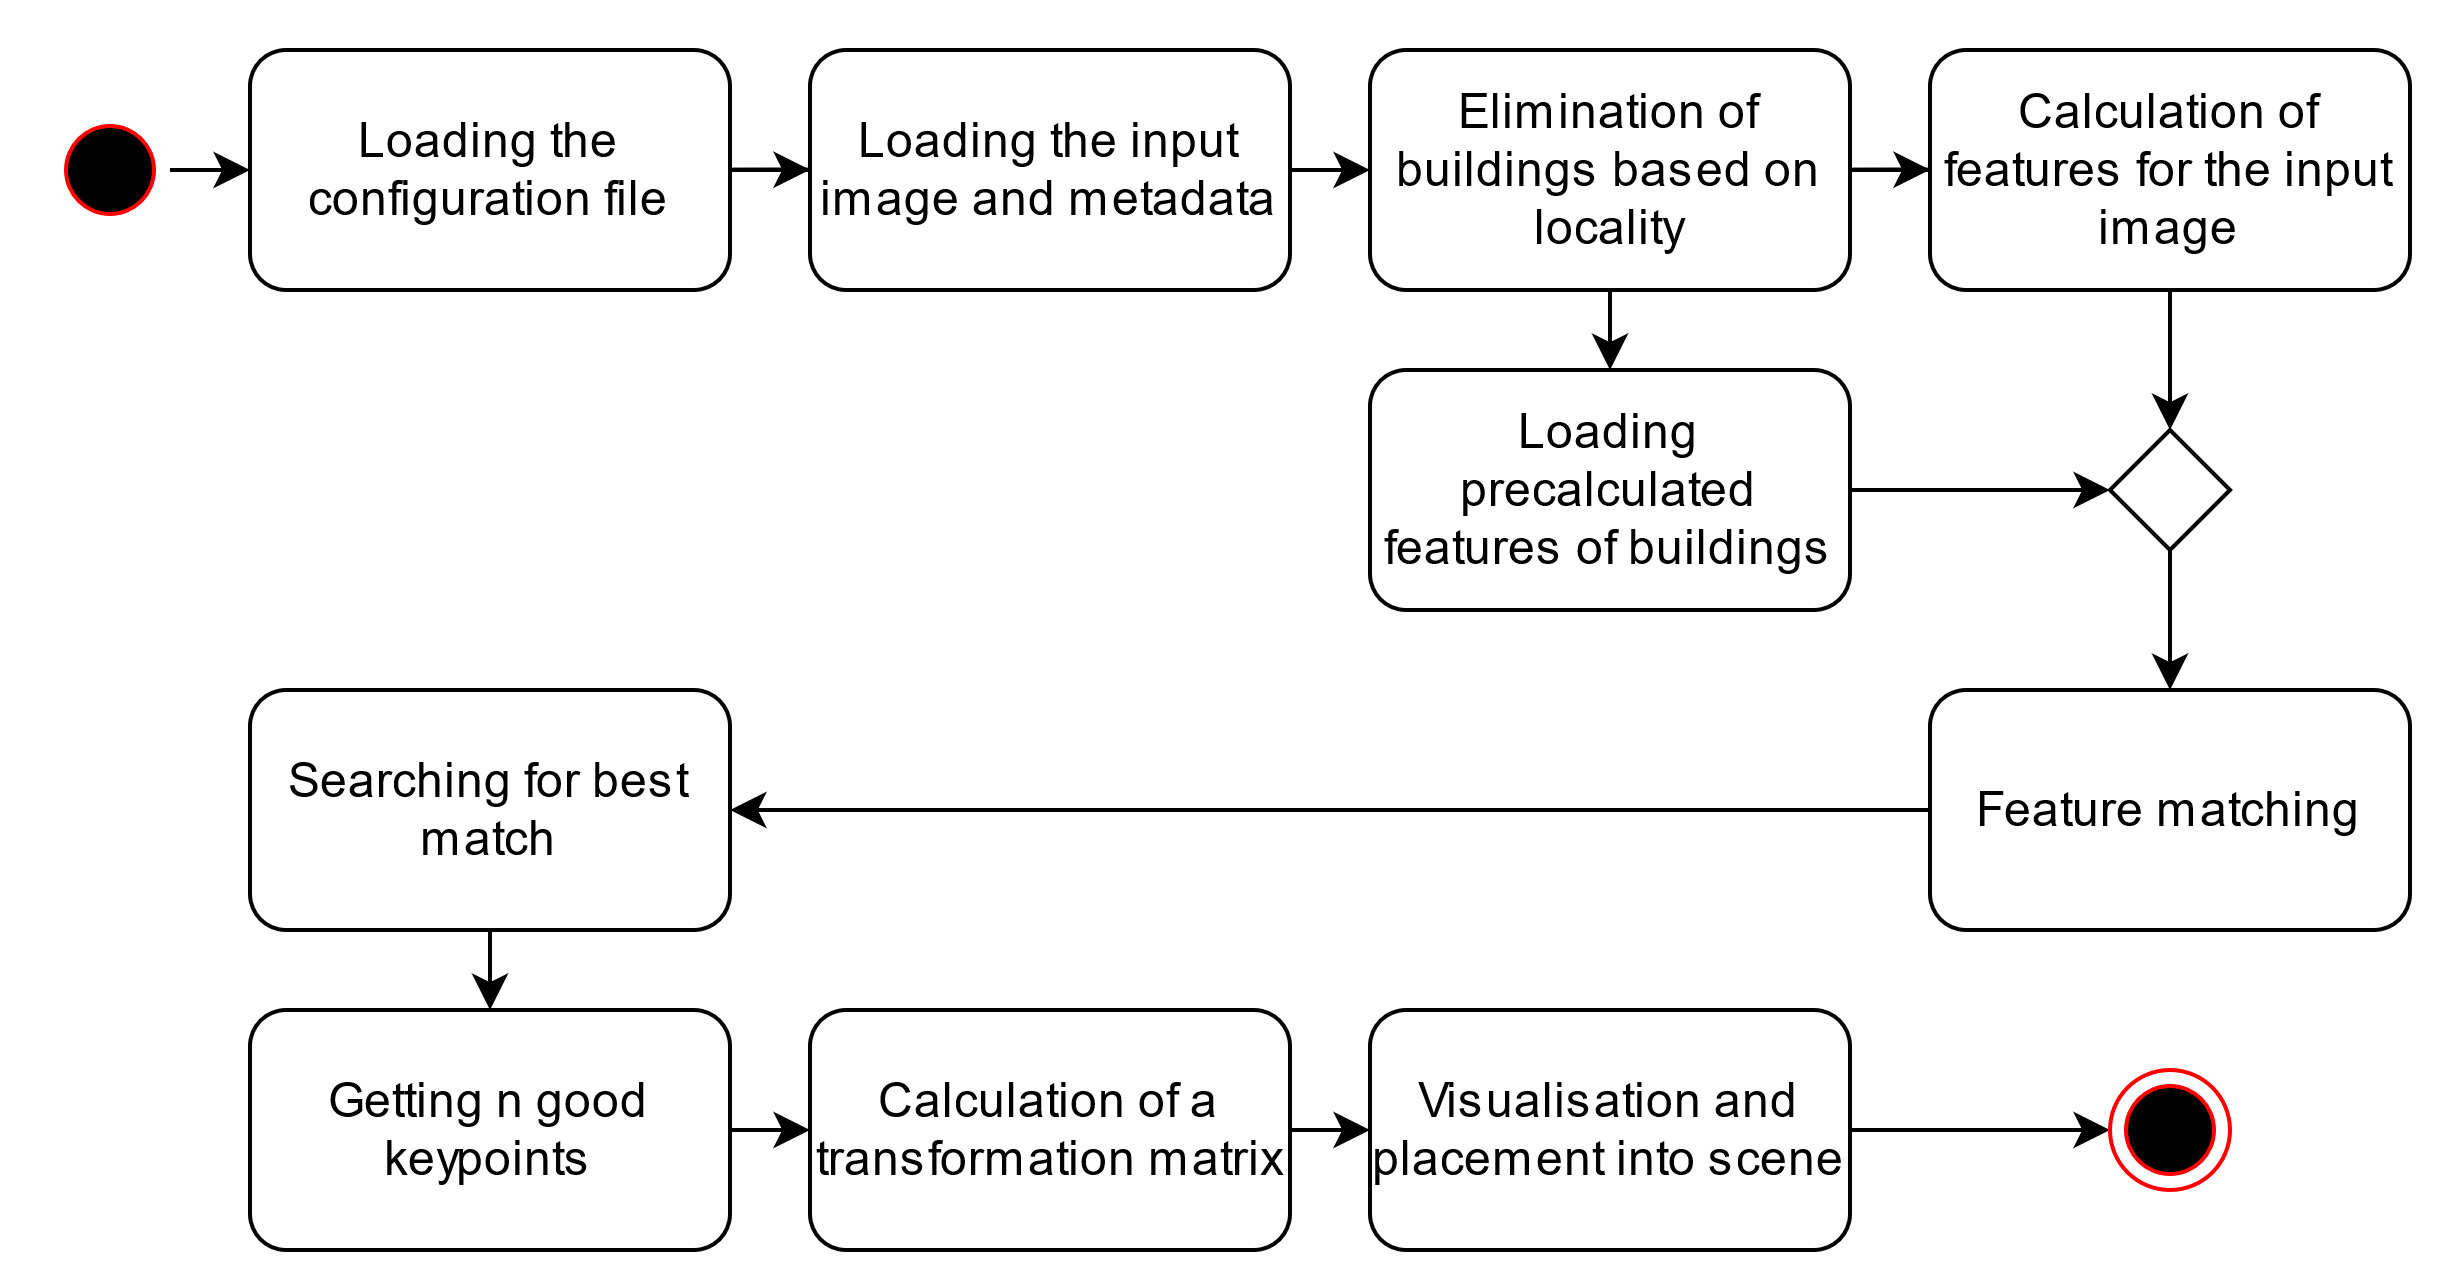
\includegraphics[width = 0.9\linewidth] {pictures/Sefcik/sefcikRealizaceDiagramAktivit.jpg}
            \caption[Activity diagram of prototype realisation of Scene Recognition and Editing bachelor thesis by Šefčík]{Activity diagram of prototype realisation of Scene Recognition and Editing bachelor thesis by Šefčík. The diagram is translated from the Šefčík's original~\cite{Sefcik2020}.}
            \label{img:sefcikDiagramAktivit}
        \end{figure}
        
        The prototype was implemented using the Python programming language and OpenCV, the library for computer vision, and the Pillow library. In the implementation, the feature detecting and extracting method SIFT and the matching based on the FLANN were used. The Lowe's ratio test and RANSAC were used to filter and smooth out the matching output.
        
        A simple file system database of images with buildings of different architectural styles was created to test the prototype. Šefčík’s thesis was concluded with that prototype testing, where the performance of the prototype was evaluated. The importance of image pre-processing was shown in the testing and the good results of CLAHE were specifically mentioned there as the only worthy method of pre-processing. It was also mentioned that using the RANSAC algorithm helps a lot with recognition accuracy. A big advantage of the RANSAC algorithm was that it neglected the bad matches that are created in repeated patterns (same windows on building).
            
    \section{Dowry Towns of Czech Queens - Core}
        The \textit{Dowry Towns of Czech Queens - Core} thesis by Daniel Vančura (in original called \textit{Věnná města českých královen - jádro})~\cite{Vancura2020} is important work for the project. This section describes the parts of Vančura's bachelor thesis in regard to ours. His thesis is then divided into chapters, in which the first chapters describe the current state before the beginning of his works and important technologies in the project. The next chapters talk about design and realisation.

       The main goals of Vančura's thesis have been:
        %
        \begin{itemize}
            \item Finishing the application programming interface (API),
            \item Refactoring the data storage,
            \item Creating documentation for the entire technical area of the project. Overall, the thesis has to be the documentation itself for other students working within the DTBQ project.
        \end{itemize}
        %
                
        \subsection{Previous state of the project}
            Among others, a principle of 3D model approval and creation is explained in Vančura's thesis. The 3D models are models of selected historical buildings that will be later prepared for the display in virtual and augmented reality. Before that, these models have to be first created with highest historical accuracy.
            
            The approval process was created, because the 3D model creator and the historian are not expected to be one person. In this process, the 3D model creator creates a model, which is then approved by a historian and graphic designer who check the correctness of the model. This process is facilitated with version control for the models, so if the model is not approved, a new version can be created. The models have to be produced for many different conditions like snowy, sunny or night. It is not suitable to display buildings with snow on it in the summer.
            
            There is also mentioned the concept of not only using a geolocation system but also computer vision for better accuracy. Vančura's thesis specifically mentions the solution by using 360\degree photos. The state description of the project at the time before his thesis is elaborated here in detail. The parts on which he worked are clearly visible in the schema~\ref{img:vancuraBigPicture} as the highlighted parts. These parts are mainly databases and private API. The public API is then simplified and the Bug API is added to  the public API. The Bug API serves the purpose of logging problems, errors and other data.
            %
            \begin{figure}
                \centering
                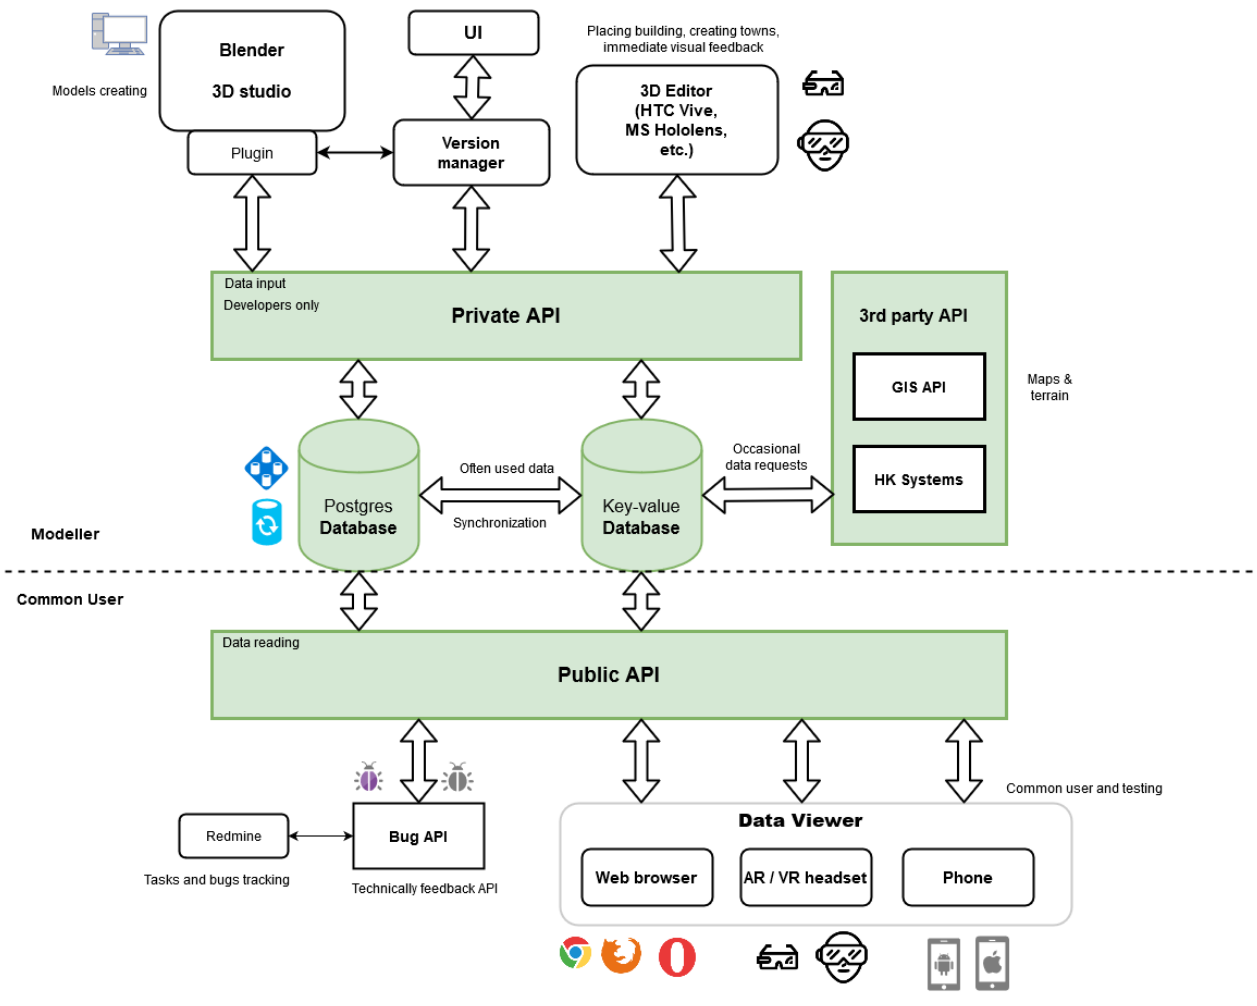
\includegraphics[width = 1\linewidth]{VancuraBigPicture.png}
                \caption[Scheme of the whole DTBQ project]{Scheme of the whole DTBQ project. Vančura's thesis covered the green highlighted parts. The scheme is from Vančura's thesis~\cite{Vancura2020}.}
                \label{img:vancuraBigPicture}
            \end{figure}
            %
            
At the time Vančura's work began, the technologies had already been determined as follows~\cite{Vancura2020}:
            \begin{description}
                \item[Docker] Tool that creates containers (environments) where the app can run independently of the outer platform,
                \item[Node.js] JavaScript multi-platform environment,
                \item[Express] Framework for Node.js that simplifies creating of the web application,
                \item[Typescript] It is a technology introducing type variables into Javascript,
                \item[TypeORM] Framework for object-relational mapping of object into database,
                \item[JSON Web Token (JWT)] Security format standard,
                \item[PostgreSQL] Open-source object-relational database system used in the project for storing metadata,
                \item[MongoDB] Database for storing binary data in the key-value style. This technology was used for storing 3D models, textures, etc.,
                \item[Geographical Information System (GIS)] This system includes maps and other data describing terrain like aerial photos or the plan of housing. This model is used to display the terrain.
            \end{description}
            %
                
        \subsection{Design and realisation}
            Within Vančura' design, the lacks of the previous solution were corrected, which were mentioned in the analysis in his thesis. The metadata database has been redesigned and the same has been done in the approval process. The version system for the models has been introduced, with the possibility to add tags on which base it would be easy to search through the objects. Last but not least, a vision of future development was outlined.
            
            Regarding the API, the lack of the private API has been fixed, like no possibility of editing or deleting records in the database. After the correction, it is possible to do all the basic CRUD (create, read, update, delete) operations. The API allows to change supported formats, but now it supports the following formats:  
            %
            \begin{description}
                \item[3D models:] blend, 3ds, max, obj, fbx, sfb, sfa;
                \item[Images:] jpg, jpeg, png;
                \item[Configuration files:] txt, config.
            \end{description}
            %      
            It is important to note that a simple manual for administrators and developers has been created within Vančura's realisation. This manual also contains an installation guide. The thesis with the manual can be considered a complete documentation of the project at that time.

\chapter{Analysis}
    In this chapter we analyse the methods from the Research chapter. We briefly test some of the methods to make a better image about them. Further, we analyse possible technologies for the development of localisation programs.

        \section{Previous theses}
            In this section, we specifically analyse previous works in the DTBQ project that have a direct influence on our work. Vančura's thesis was important for us as an introduction to the whole project and all its characteristics, but we do not analyse it. Instead of it, we analyse the works directly preceding our.            

            \subsection{Urban scene recognition and editing I}
                As mentioned above, the \textit{Urban scene recognition and editing} thesis by Jan Šefčík~\cite{Sefcik2020} is the direct predecessor of our thesis which continues in Šefčík's footsteps. Within analysis, we take a look at what is worth keeping and what is good to further analyse, improve or do differently.
                
                \subsubsection*{Analysis}
                The analysis describes which pre-processing methods are useful and which are not. We see this part as important, because the pre-processing is a part of the image processing and it should not be omitted, as Šefčík's thesis mentions. Šefčík also mentions that the only pre-processing method that makes a viable positive difference is the \textit{Contrast Limited Adaptive Histogram Equalisation} (CLAHE) because it helps to compensate for the bad exposition or shadows. The feature detecting and describing methods have been well analysed too. Further, in his thesis only the SIFT algorithm, because it was evaluated as the most accurate one.
                
                \subsubsection*{Design and realisation}
                In the analysis, we lack an explanation why FLANN was used for feature matching, so we will analyse if it is an ideal choice. Besides many other pieces of advice that we follow, there was the design and realisation of an image recognition prototype. The prototype was created in Python, which is not a typical programming language used to develop mobile applications. We believe that Python was chosen mainly for the purposes of the prototype and not for possible use in a mobile application. Based on that, we decided to further analyse what technologies and methods to use.
                
                Šefčík created an image database as part of the prototype implementation. It contains buildings of different sizes or architectural styles. The database also contains additional information about the photos, such as the GPS coordinates of the place where the photo was taken. Šefčík mentions that GPS coordinates are key for speeding up the detection process. Based on the location, it is then possible to disqualify many buildings, so there will be significantly less buildings to search by using the computer vision.
               
                \subsubsection*{Testing}
                In the end there was done testing on the database. The best results of Šefčík’s work may be seen in the image~\ref{fig:Sefciks_prototype_results}. The results seem accurate in most cases. There are only a few images of the whole database so we consider that it is the showcase of the best results.
                
                \begin{figure}
                    \centering
                    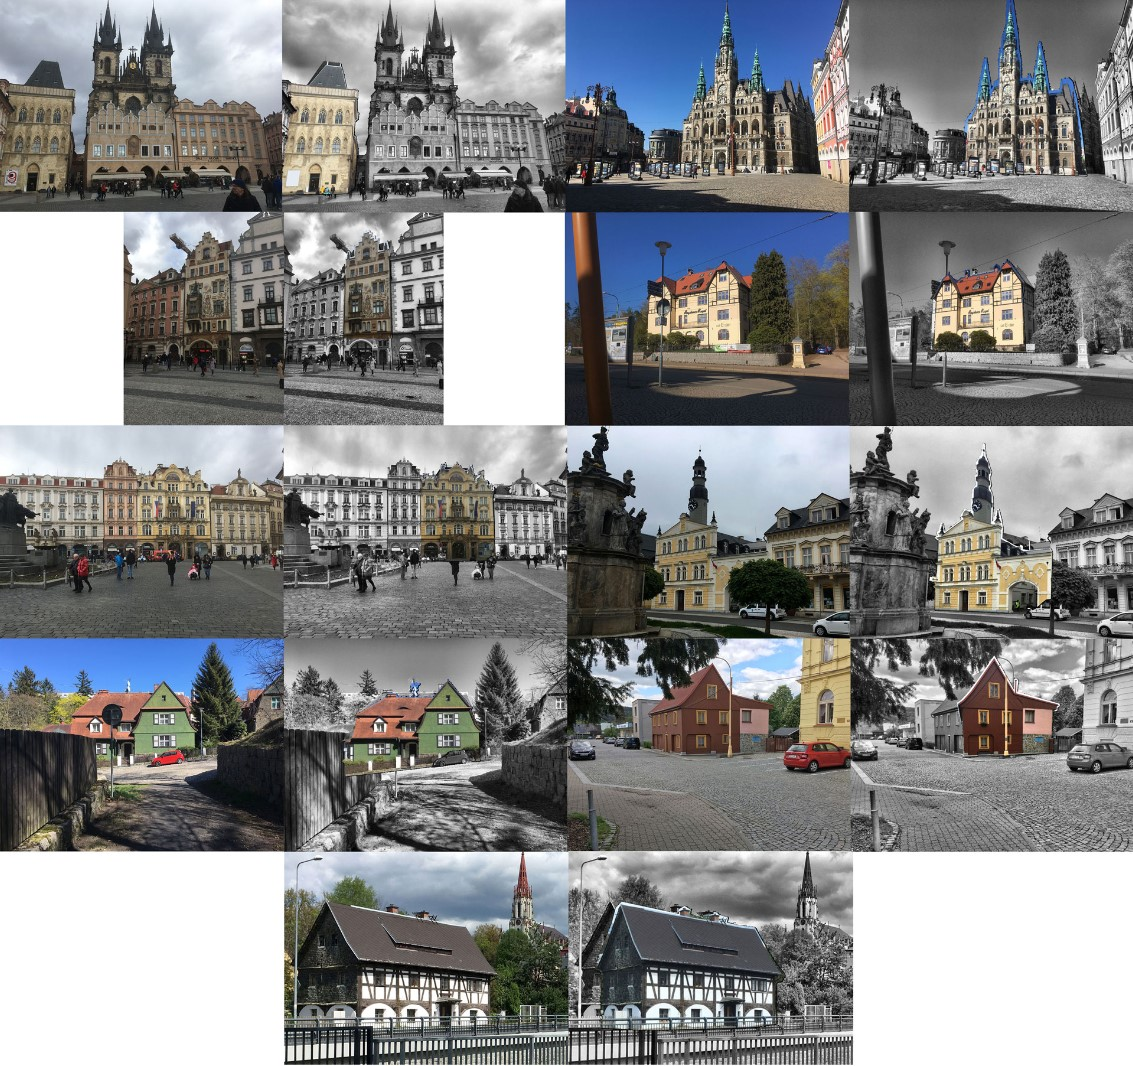
\includegraphics[width = 1\linewidth]{pictures/Sefciks_prototype_results.jpg}
                    \caption[Performance of Šefčík's prototype]{Performance of Šefčík's prototype. Photo collection was made by Jan Šefčík~\cite{Sefcik2020}.}
                    \label{fig:Sefciks_prototype_results}
                \end{figure}

                However we see testing as the main weakness of Šefčík's work. Every reference image was created from an image that is queried to be recognised only by blackening the parts of the image that are not the building itself. So for every queried image with a building, there exists a perfect matching reference image and thus no transformation invariance is tested except scale. This is in contrast with the use outside of the experimental environment.
                
            \subsection{DTBQ - Image recognition module} \label{sec:stepan}
                Šefčík's thesis is not the only important one on which ours continues. Another important one is the master thesis of Jaroslav Štěpán~\cite{Stepan2019}. There are three goals that are important to us, namely creating the localisation module, the tracking module and the manual on how to make a module in the application. In the localisation module and tracking module goals is hidden another goal which is to create the Application Programming Interface (API) that would be used by the modules. The API would give the solutions addressing common problems of the modules.
                
                \subsubsection*{API}
                The API would provide support in the following areas: access to the camera of the phone, access to the phone sensors, connection to the network and access to the stored data. All the provided interfaces by the API are visible in the diagram in the figure~\ref{fig:Jaroslav_Stepan_localisation_module}. The diagram is a part of a design of the localisation module that was developed as a part of his thesis. At the top of the diagram are the interfaces that provide help to the localisation module, but also the interfaces that have to be implemented by the localisation module.
                
                Specifically, the \texttt{INetworkProvider} interface provides the module the possibility to communicate with remote servers or to establish network connections. Another \texttt{ICameraProvider} interface provides the access to the camera or the properties of the camera in the form of camera intrinsic parameters. The other two supporting interfaces are \texttt{ISensorProvider}, which provides easy access to the data from phone sensors, and \texttt{IStorageProvider}, which accesses the stored data to the module. All these interfaces have the same purpose and that is to make it easier to develop modules. This is done in this way, these interfaces are simple and easy to use. We see this as very useful, because we do not have to have a lot of knowledge about Android programming when developing our module. These interfaces take care of that.
                
                \subsubsection*{Localisation module interface}
                But probably the most important interface is the \texttt{LocalizationModule}, which has to be implemented by the localisation module. We see the \texttt{getGlobalPosition} method as the main of the three methods there, because it is the method called by the application to get the location of the phone. The other methods are there to provide the application information about the module, which is also important, but is not the core of the module's purpose.
                
                \subsubsection*{Realisation of a simple localisation module}
                In the diagram in the figure~\ref{fig:Jaroslav_Stepan_localisation_module} also contains the design of the localisation module. The design in the part of Recognition is rather simple, but it sufficiently outlines the main properties of the main processing part like feature (called keypoint in the diagram) detection and feature description. There is also a method that is named \texttt{findObject} and its arguments are the features. We do not see this as completely clear, because features are not compared themselves, but their descriptors are what should be compared to find similarities in images.
                
                
                \begin{figure}
                    \centering
                    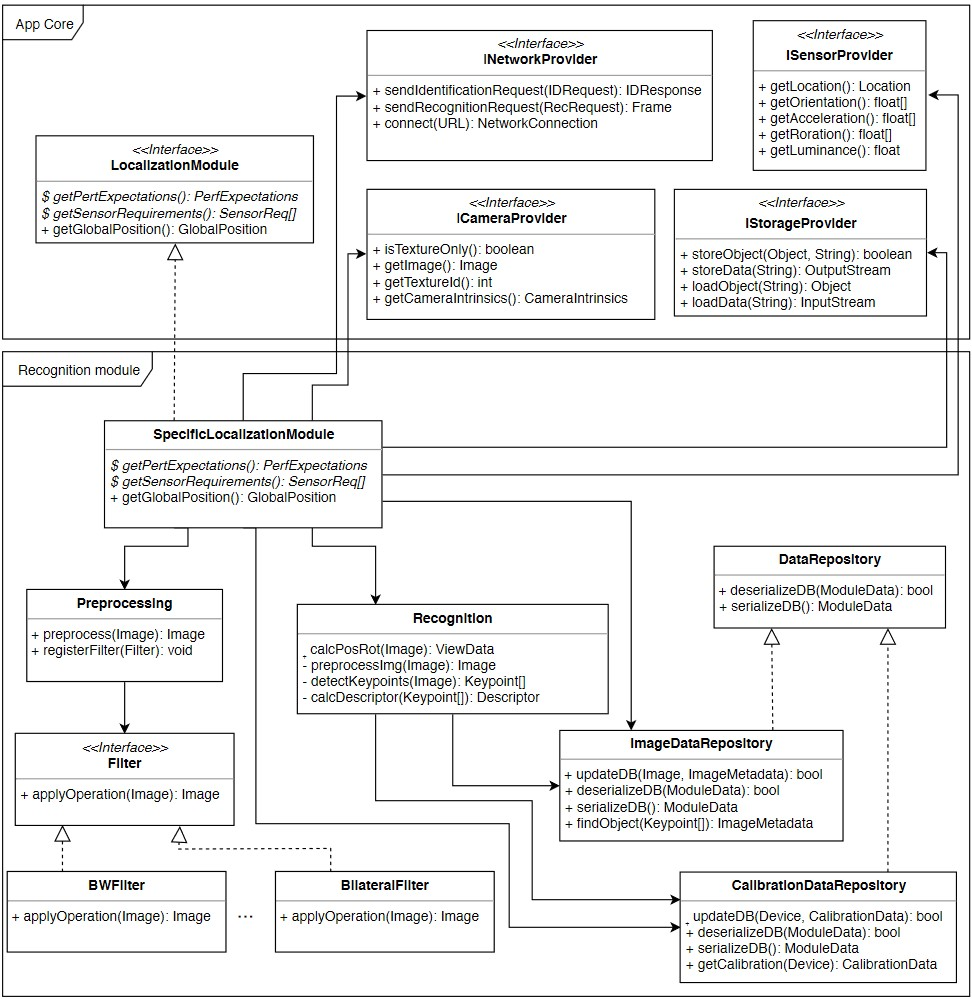
\includegraphics[width = 1\linewidth] {pictures/Jaroslav_Stepan_localisation_module.jpg}
                    \caption[Localisation module class diagram of the thesis named \textit{DTBQ - Image recognition module}]{Localisation module class diagram of the thesis named textit{DTBQ - Image recognition module}. Diagram is taken from the thesis created by Jaroslav Štěpán~\cite{Stepan2019}.}
                    \label{fig:Jaroslav_Stepan_localisation_module}
                \end{figure}
                
                There is a part of implementation that deals with pre-processing. All the pre-processing methods have to implement the interface. Based on Šefčík’s thesis, we think that the filters could be scaling, CLAHE, and conversion of color images into grayscale ones. Štěpán states that the image is given by the mobile device in the YUV model and it is needed to convert it to RGB and then to shades of grey. He does not explain why the conversion to RGB is needed and we do not see the need to do so. The conversion to the shades of grey is necessary because all the considered feature detection and extraction algorithms are defined only for grayscale images. The separation of the Y channel (brightness) from the YUV color model should be a sufficient and simple way to create input grayscale images. However, it is important to note that it would be needed to store the descriptors of objects' pictures (of buildings or other objects to be found) in the database that would be computed also from the Y channel (Y from the YUV color model). This detail might not be necessary, but the disunity could lead to lower accuracy.
                
                \subsubsection*{Localisation module developing}
                At the end of the realisation in the Štěpán’s work, there are instructions on how to create a module for the DTBQ application. Thanks to these instructions the requirements of knowledge of Android development are lower. The manual expects the developer to use the C++ programming language for the main computations, so the manual also contains part on how to exchange data between code in Java programming language (Java is the main programming language of the application) and the C++ programmed part.
                
        \section{Computer vision libraries}
                In the preceding work by Jan Šefčík~\cite{Sefcik2020} was not done any analysis regarding the libraries, platforms or software development kits in the area of computer vision. OpenCV was introduced without any comment on exactly why to use this library, thus we analyse not only this library but also some others. Finally, we can make a reasoned decision on what to use in realising our project.
            
            \subsection{OpenCV}
                OpenCV (Open Source Computer Vision Library) is an open source library in the field of computer vision and machine learning. OpenCV is designed to provide the infrastructure for computer vision applications. OpenCV is very suitable for use in our thesis, because it provides infrastructure in the same area as the application module that would be done in our work~\cite{aboutOpenCV}.
                
                OpenCV versions up to version 4.4.0 are licensed under the 3-clause BSD license and versions since 4.5.0 are licensed under the Apache 2 license~\cite{OpenCVLicense}. Both licenses allow both non-profit and commercial use including possibility for modifications~\cite{ApacheLicense2},~\cite{BSD-3-Clause}.
                
                What we see as the benefits of OpenCV is a huge community of 47 thousand developers and more than 2500 implemented algorithms~\cite{aboutOpenCV}. We are mainly interested in feature detecting, extracting, and matching algorithms. All of the algorithms that we are interested in are implemented in OpenCV. Functionality very similar to something we want to achieve is implemented in a tutorial in the official OpenCV documentation~\cite{Huaman2021}.  There is a small demo of how to find a known object in a picture. The result of this demo can be seen in this image~\ref{fig:OpenCV_Feature_Homography_Result}. This is the major thing that we want to achieve in our work.
                
                \begin{figure}
                    \centering
                    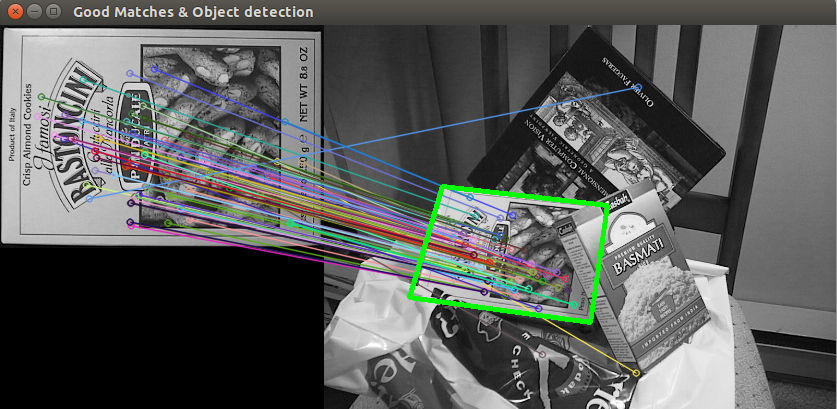
\includegraphics[width = 0.7\linewidth] {pictures/OpenCV_Feature_Homography_Result.jpg}
                    \caption[Result of a demo from OpenCV tutorial on how to find known object location in picture]{Result of a demo from OpenCV tutorial on how to find known object location in picture. Picture is from the OpenCV tutorial~\cite{Huaman2021}.}
                    \label{fig:OpenCV_Feature_Homography_Result}
                \end{figure}
                
                It is important for our project that OpenCV supports Android and besides that it also supports Windows, Linux and Mac OS. There is also a wide range of programming languages for which there exists an official interface. These languages are C++, Python, Java and MATLAB~\cite{aboutOpenCV}.
                
            \subsection{ML Kit}
                Google offers multiple products to ease up mobile application development. One of these products is the ML Kit package~\cite{Google_ML_Kit}. ML in the name means machine learning. The ML Kit is a software development kit (SDK) designed to provide solutions for the common problems in computer vision. The package supports Android and MacOS platforms and it is offered for free under the terms of Google.
                
                The ML Kit provides solutions in multiple areas, two of which are interesting to us. The first one is \textit{image labeling}. The labels assigned to images are in the form of pairs of text and probability, as can be seen in figure~\ref{table:ML_Kit_image_labeling_example}. The text describes things that might be in the image or what happens in the image. The probability then represents the self-confidence of the algorithm with the label. This is an interesting functionality, but not very suitable for the localisation.

\begin{figure}
    \centering
    \begin{minipage}[]{.312\linewidth}
        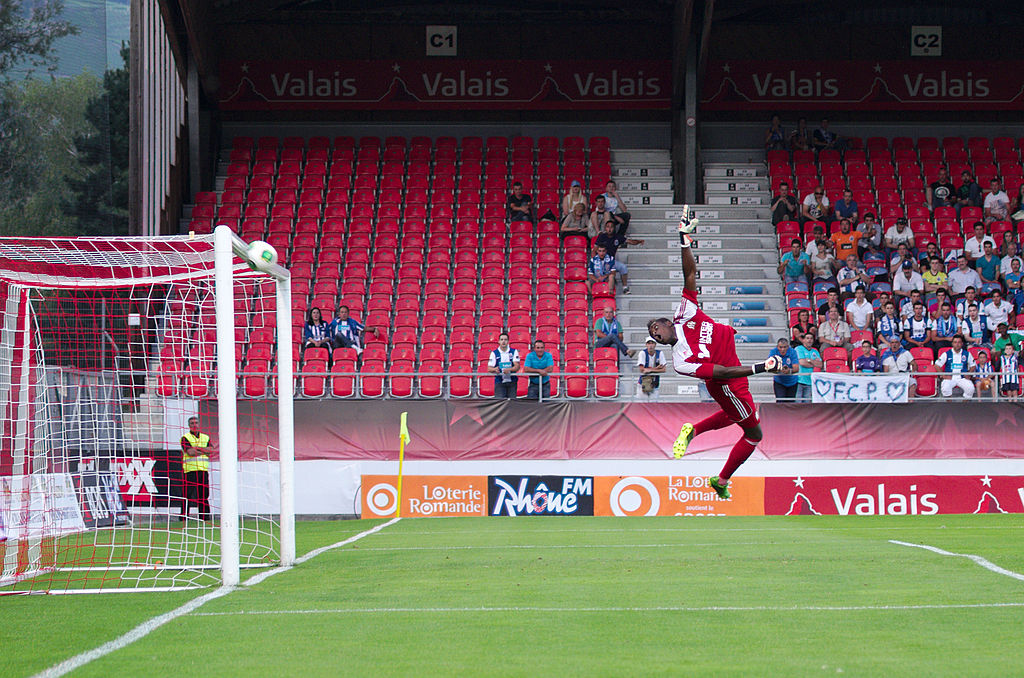
\includegraphics[width = \linewidth] {pictures/1024px-Valais_Cup_2013_-_OM-FC_Porto_13-07-2013_-_Brice_Samba_en_extension.jpg}
    \end{minipage}
    \begin{minipage}[]{.472\linewidth}
\begin{tabular}{|l|l|l|}
\hline
\textbf{Labels} & \textbf{Text} & \textbf{Confidence} \\ \hline
1               & Stadium       & 0.9205354           \\ \hline
2               & Sports        & 0.7531109           \\ \hline
3               & Event         & 0.66905296          \\ \hline
4               & Leisure       & 0.59904146          \\ \hline
5               & Soccer        & 0.56384534          \\ \hline
6               & Net           & 0.54679185          \\ \hline
7               & Plant         & 0.524364            \\ \hline
\end{tabular}
    \end{minipage}
    \caption[ML Kit \textit{image labeling} example]{Example of the ML Kit \textit{image labeling} of an image with soccer match. Example is taken from the website of the ML Kit.}
\label{table:ML_Kit_image_labeling_example}
\end{figure}

            Another interesting area for us is the \textit{detection and tracking}. In this functionality, the ML Kit provides more information about what is in the image than in the \textit{image labeling}. The output of detecting and tracking can be seen in the figure~\ref{fig:ML_Kit_object_detection_tracking}. The ML Kit provides tracking and detection of multiple objects in one photo. The output consists from the tracking ID of the object, boundaries of the area where the object is detected, and a label (similar to one in the \textit{image labeling}). There is one main disadvantage, because the boundaries are only in the form of a bounding box. The bounding box provides too low accuracy for our intentions. There is no other positioning information than the scale and approximate location. Also, the use of the detecting and tracking is not in line with what we expect, because we want to detect objects from our own database and the ML Kit  detects objects categories only from its internal database.
            
            \begin{figure}
                \centering
                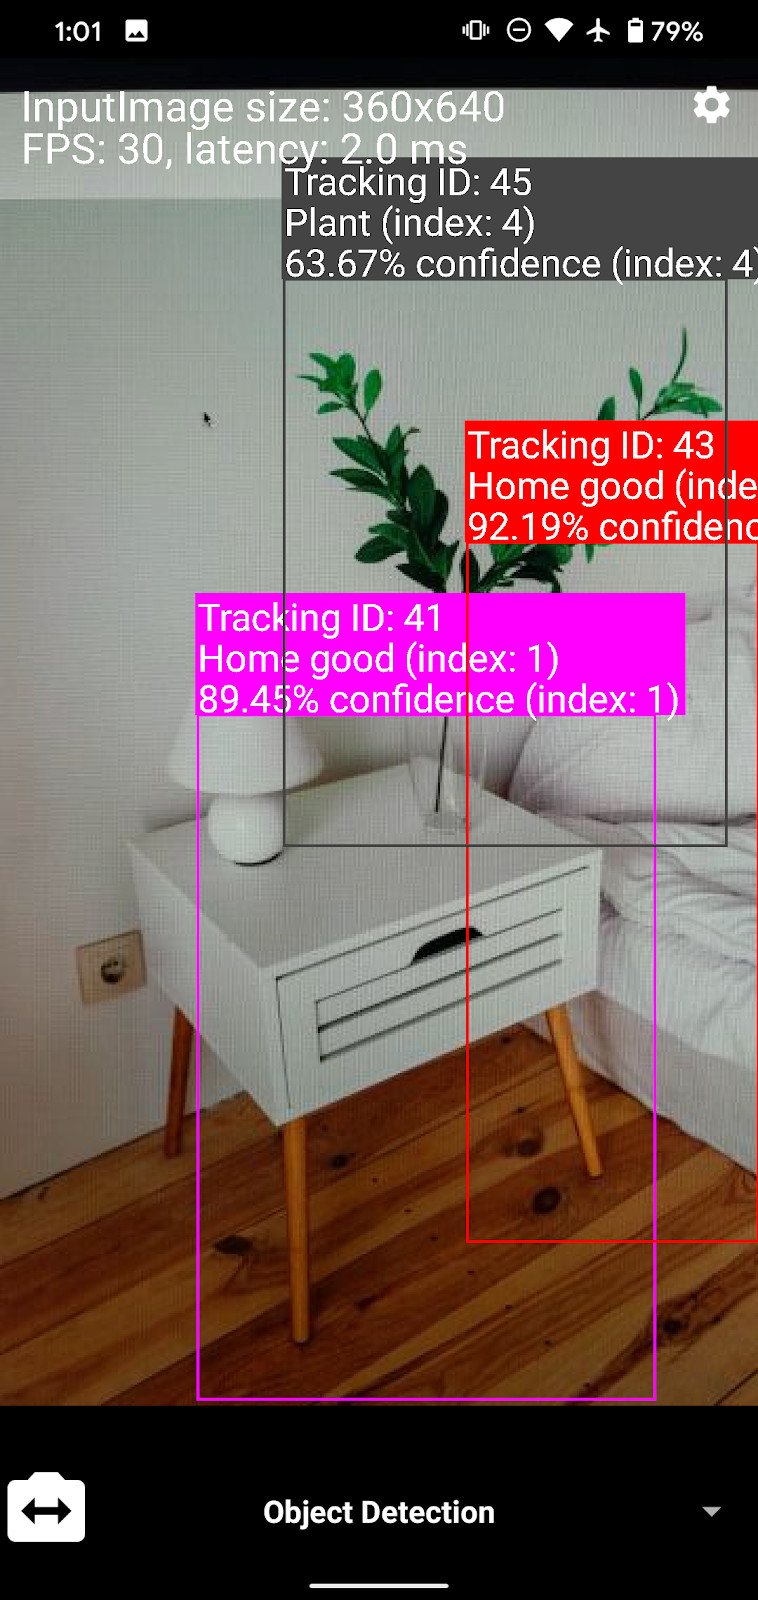
\includegraphics[width = 0.4\linewidth, height = 0.8\linewidth] {pictures/ML_Kit_quickstart-object-detection.jpg}
                \caption[Example of ML Kit \textit{detection and tracking}]{Example of ML Kit \textit{detection and tracking}. Example is taken from the samples provided by Google on the ML Kit website.}
                \label{fig:ML_Kit_object_detection_tracking}
            \end{figure}
            
            The ML Kit shows as capable but it provides less specialised solutions than we need. So we do not consider using ML Kit any further.
            
            \subsection{ARCore}
                ARCore is a platform created by Google for the implementation of augmented reality projects~\cite{Google_ARCore}. Augmented reality is also what the DTBQ mobile application is about. The first from the ARCore's three main elements of performance is the \textit{motion tracking}. It covers the area of keeping the knowledge of the relative position of the camera in the surroundings. \textit{Environmental understanding}, the second element of ArCore, is responsible for understanding the shapes of the surroundings. It mainly detects planes and the geometry of the world around. Performance of \textit{light estimation}, the last element, is clearly visible in the image~\ref{fig:Google_ARCore_App_example} where the animals create shadows on the floor in a realistic style. The~images~\ref{fig:Google_ARCore_App_example} are taken from a typical mobile application that uses ARCore. The application renders animals in the images of the real world in real-time. It also uses two other elements of the ARCore \textit{motion tracking} (users can move phones around an animal) and \textit{environmental understanding} (animal stands on flat ground).

                ARCore is ideal for a tracking module of the DTBQ mobile application. That is probably why it was chosen for the tracking module in the work of Jaroslav Štěpán~\cite{Stepan2019}. But we want to localise buildings in the picture and such functionality is not implemented in the ARCore, thus we no longer consider ARCore in our work.
                
                \begin{figure}
                    \centering
                    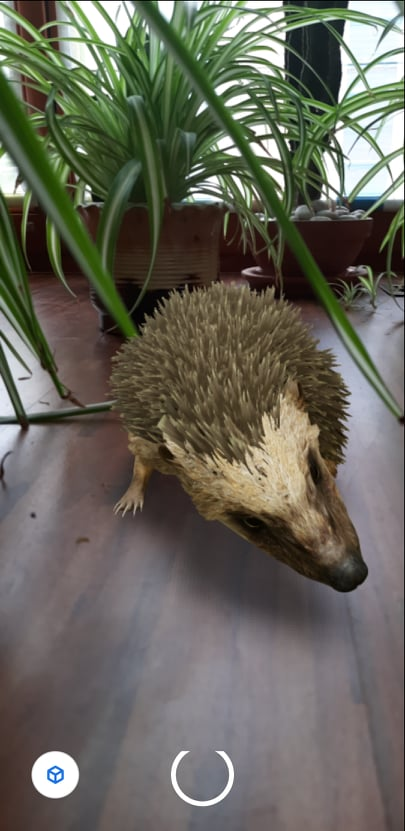
\includegraphics[width = 0.34\linewidth] {pictures/Google_ARCore_App_Example.jpg}
                    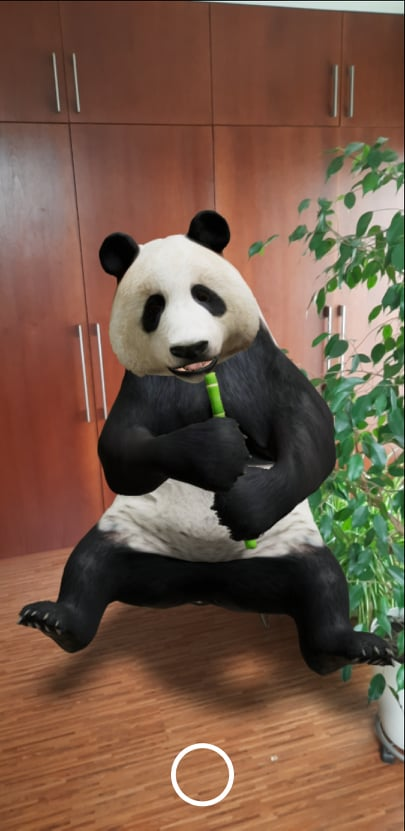
\includegraphics[width = 0.34\linewidth] {pictures/Google_ARCore_App_Example2.jpg}
                    \caption[Example of an application based on ARCore]{Example of an application based on ARCore. Images are screenshots from a phone application created by Google LLC.}
                    \label{fig:Google_ARCore_App_example}
                \end{figure}
                
            \subsection{Conclusion}
                We have analysed the OpenCV, ML Kit and ARCore, but the only acceptable option was the OpenCV, because the other two products have not met our requirements.
            
        \section{Programming language}
            Since we have decided to use OpenCV, we have to use some programming language that is supported by OpenCV. The supported languages are C++, Python, Java and MATLAB~\cite{aboutOpenCV}. We eliminated MATLAB as not suitable and it is not mentioned here. Main reason is non-existent possibility of application development on the Android platform.

            \subsection{C++}
                In our work we are implementing a module to the DTBQ application. Jaroslav Štěpán has already introduced instructions on how to create a module for this application using C++~\cite{Stepan2019}. Therefore, if we used C++, we would not need to research how to create the module ourselves completely but we could just follow Štěpán’s instructions. Another advantage is that the DTBQ application is a real-time application and C++ is a viable choice for real-time applications. The programming language is generally known for its efficiency, so in case of programming our own processing methods the high computation speed is easily achievable.
                %VHODNE K UVÁŽENÍ
                    %CPU VS GPU
                    %výkon porovnani ruznych implementaci algoritmu? OPENCV vs others..

            \subsection{Java}
                The DTBQ mobile application for Android is developed using Java~\cite{Stepan2019}. Java is also an official language for developing Android applications. This is a big advantage that speaks for the use of Java. But Java is an interpreted language and such languages generally run slower than compiled languages like C++. Therefore, if we want to code some algorithms not implemented in the OpenCV, it would lead to longer computation times. Our project creates a module in real-time application, in which speed is critical, and in the mentioned case of implementing our own algorithms could be the use of Java a big problem. But according to Štěpán's instructions at least some code would be needed in Java as an intermediary between the application and the C++ in case of developing application module~\cite{Stepan2019}.
                
            \subsection{Python}
                In the case of Python, the advantage for us lies in the fact that Python was already used by Jan Šefčík~\cite{Sefcik2020} and his thesis is the direct predecessor of ours. Thanks to that, it would be possible to continue on the basis of Šefcik's code and develop it further. That is a major advantage. However, there is also one main downfall. In case of using Python, we would need to port that to Android ourselves, because the DTBQ application now supports only C++ or Java modules~\cite{Stepan2019} and there are no instructions on how to create modules for the DTBQ application in Python.

        \section{Feature detecting, extracting and matching methods}
            %TODO do a description of this section
            \subsection{Feature detecting and extracting}
                There are many methods for detecting and describing features. In the previous thesis by Šefčík~\cite{Sefcik2020} were analysed ORB, SIFT and SURF. His thesis concluded that the most accurate method of feature detection is SIFT. However, it is also stated that it is the slowest one among the three methods. The fastest one is ORB. The SURF method is commented as not suitable for the DTBQ project, because the method is patented and it does not bring any significant advantages over the other two methods that are free to use.
                
                \subsubsection*{Methods not yet considered}
                What is not mentioned in Šefčík's work is the SIFT modification called RootSIFT and feature description method called BEBLID.
                 
                RootSIFT is considered more accurate than SIFT with neglectable computation time increase. It is not included in OpenCV, but it is not complicated to implement it when the SIFT implementation is available, so we could implement it ourselves.
                
                BEBLID was introduced recently, in the year 2020. At the time Šefčík did his thesis, this method was not included in the OpenCV like other methods. This method is implemented in OpenCV in modules with experimental and non-free algorithms, because it is considered an experimental method. But the method itself is free and it was published with the 3-clause BSD license~\cite{Suarez2020_GitHub}. To use this method, a compilation of the OpenCV with this module is needed. According to the documentation, this compilation with extra modules is also possible for Android. But anyway, the algorithm is published in the online Git repository in the form of a demo~\cite{Suarez2020_GitHub}. The demo was created using OpenCV and C++, so possible integration into our work should be without any problems in a case of using C++. The descriptors can be used to describe features detected by ORB or SIFT methods.
                
                We do not consider to use any deep learning methods of feature detecting and extracting in our work. The application has to run in real-time on smartphones, where the resources are limited and the computational costs of running deep learning methods are increased significantly in comparison to \textit{handmade methods}\cite{SUAREZ2020_paper}.

            \subsection{Feature detecting and extracting in OpenCV}
                All the feature detecting and describing methods in OpenCV can be easily exchanged, because they implement the \texttt{Feature2D} interface. So the choice of the method can be done later or the choice can be configured at runtime. But since we are interested in a real-time application, the speed of the feature detection and description is important.
                
                \subsubsection*{Testing}
                An early prototype was implemented using OpenCV to test the speed of the methods. For testing we used a subset of images from the image database of the Šefčík's project~\cite{Sefcik2020}. We did 5 tests and in each one there was one scene image (urban scenery) and a database of reference building images, which were searched in the scene.
                
                The number of detected features was limited to 1000. The number was slightly lower for several images, because the methods were not always able to find 1000 features (we observed that ORB is more reliable in detecting at least 1000 features than SIFT). After detecting the features, the features were described with a predetermined algorithm and the time that the process took was carefully measured.

                Each of the object descriptor vectors was then compared with the calculated one from the scene image. The object that best suited (according to simple metric) to the scene was chosen and displayed in the scene. After that we could visually evaluate if the display of the object in the scene is correct or not the same, as can be seen in images~\ref{fig:featureMatchingYesNo}. This test was primarily prepared in mind to measure the time. The accuracy measurement was simplified to a binary evaluation: fail or success.
                
                \begin{figure}
                    \centering
                    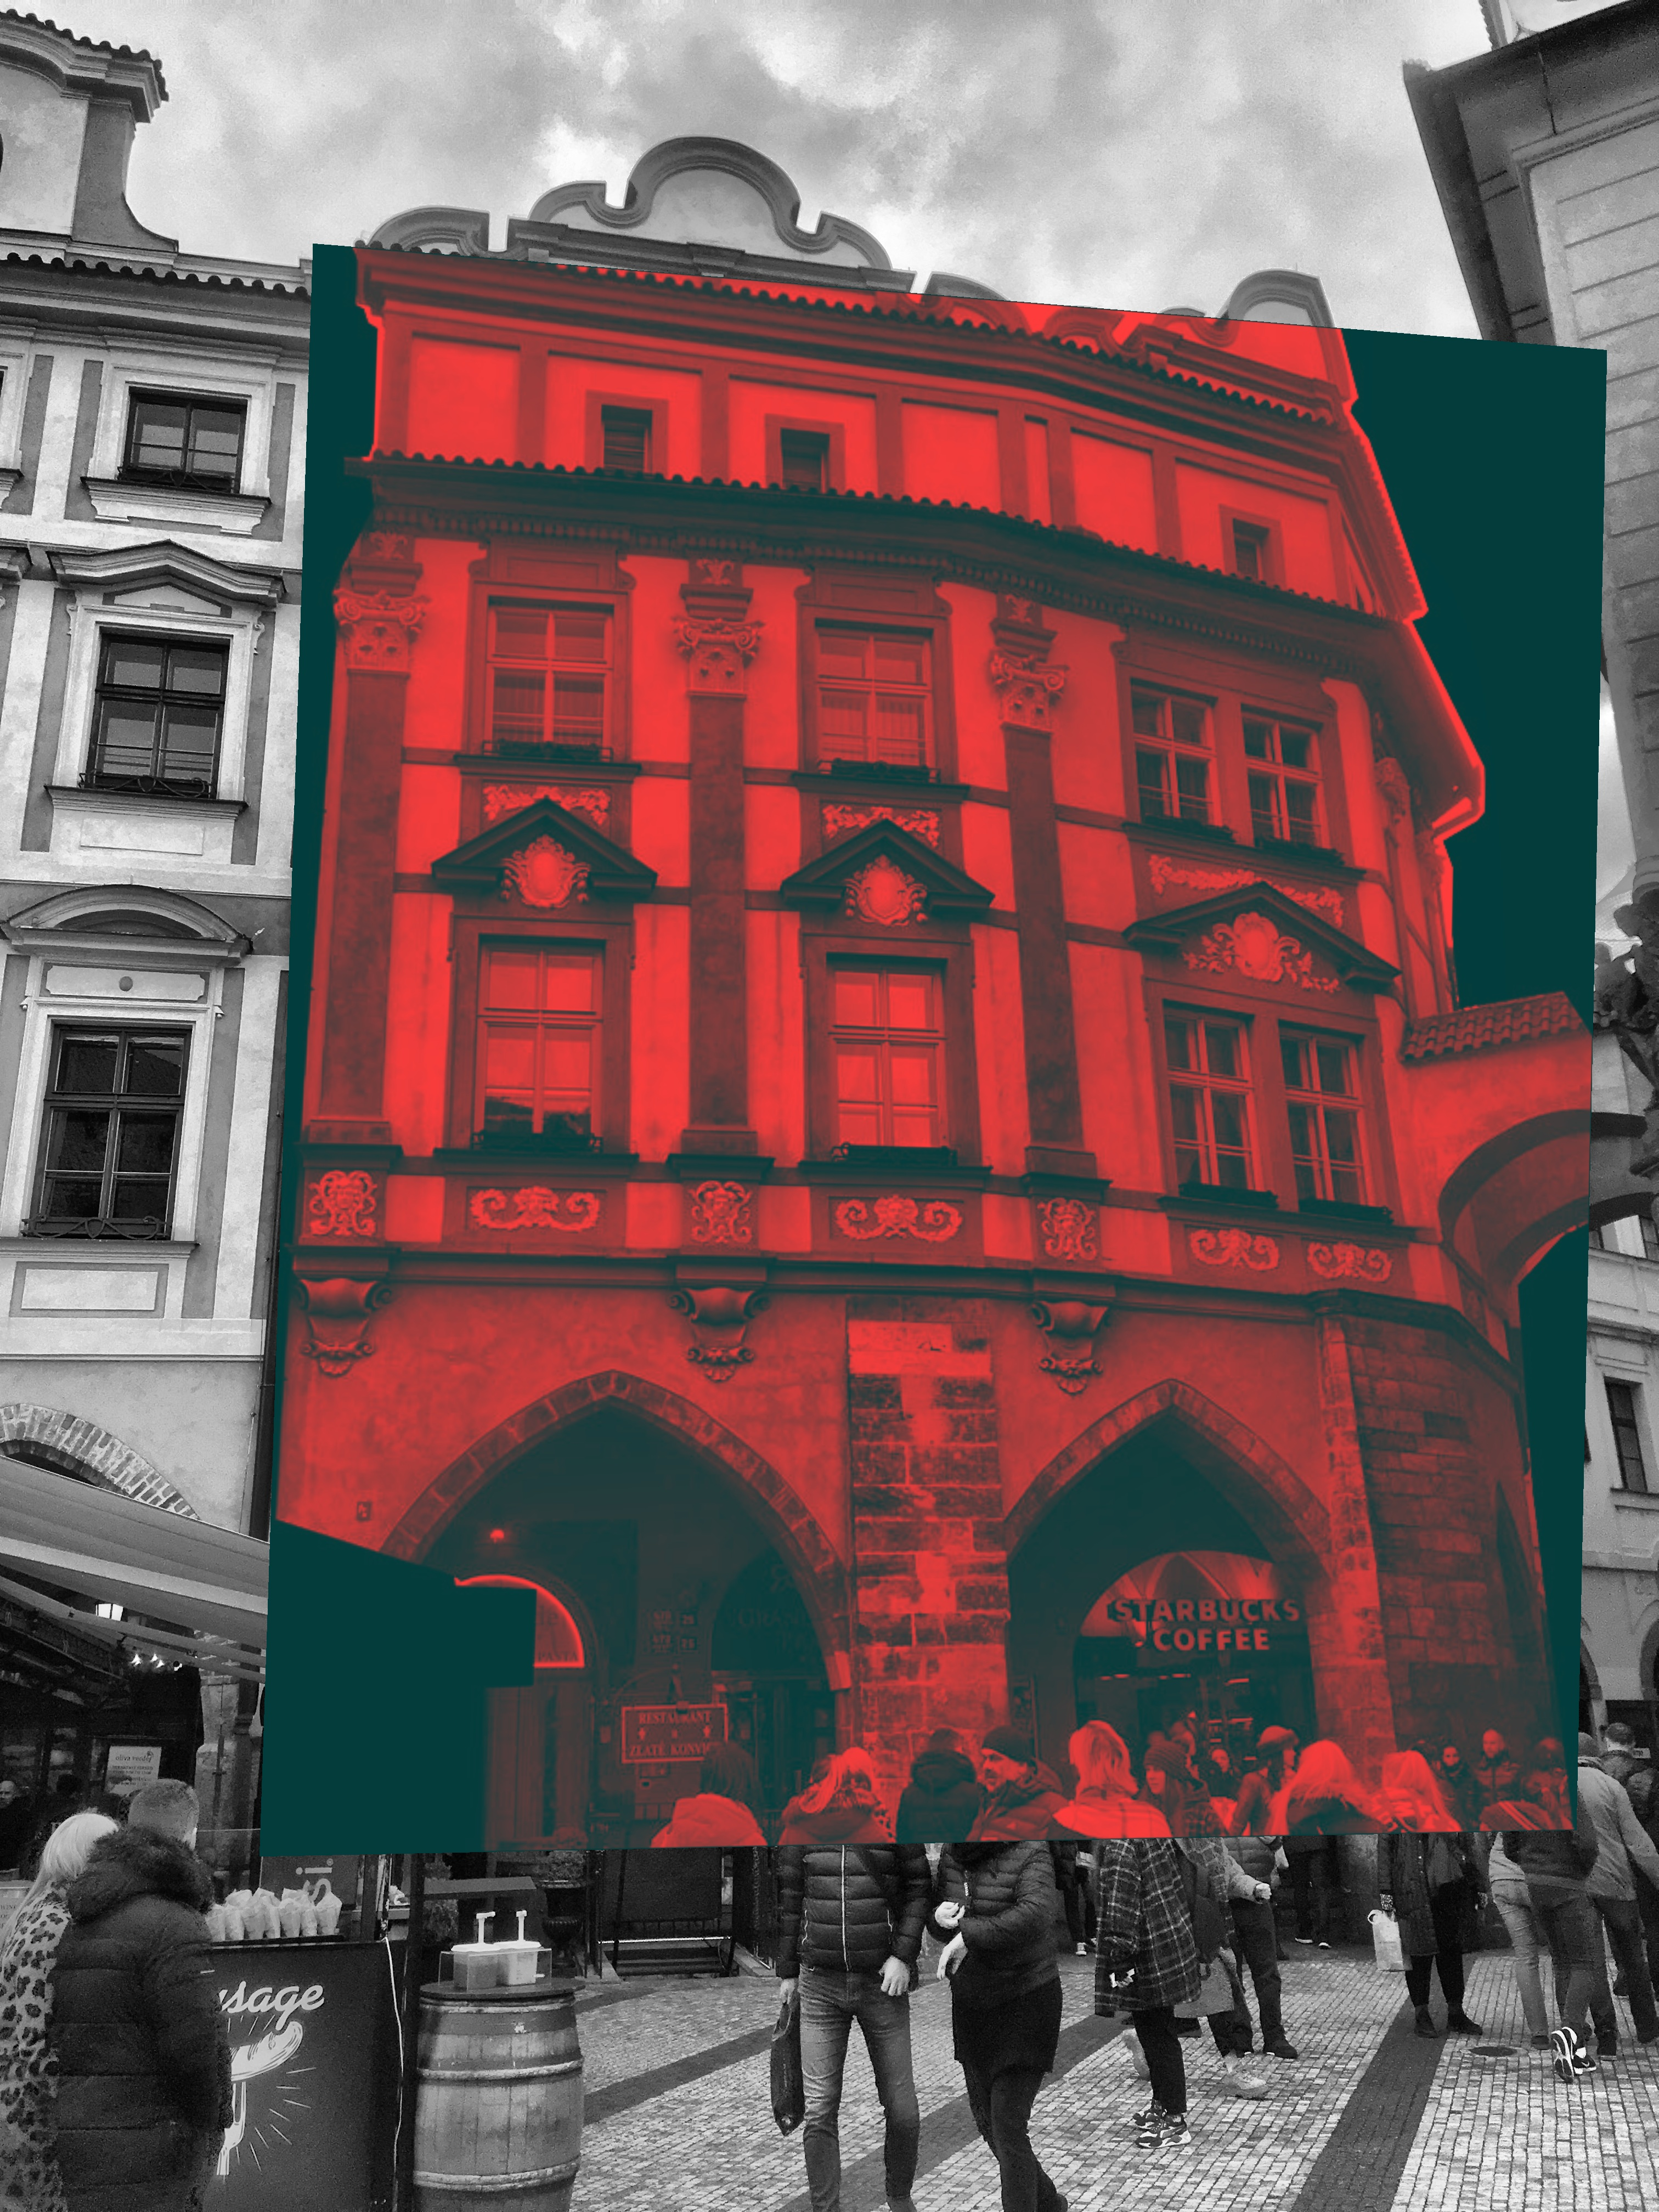
\includegraphics[width = 0.39\linewidth] {pictures/ORB_ORB_BF_2_img1.jpg}
                    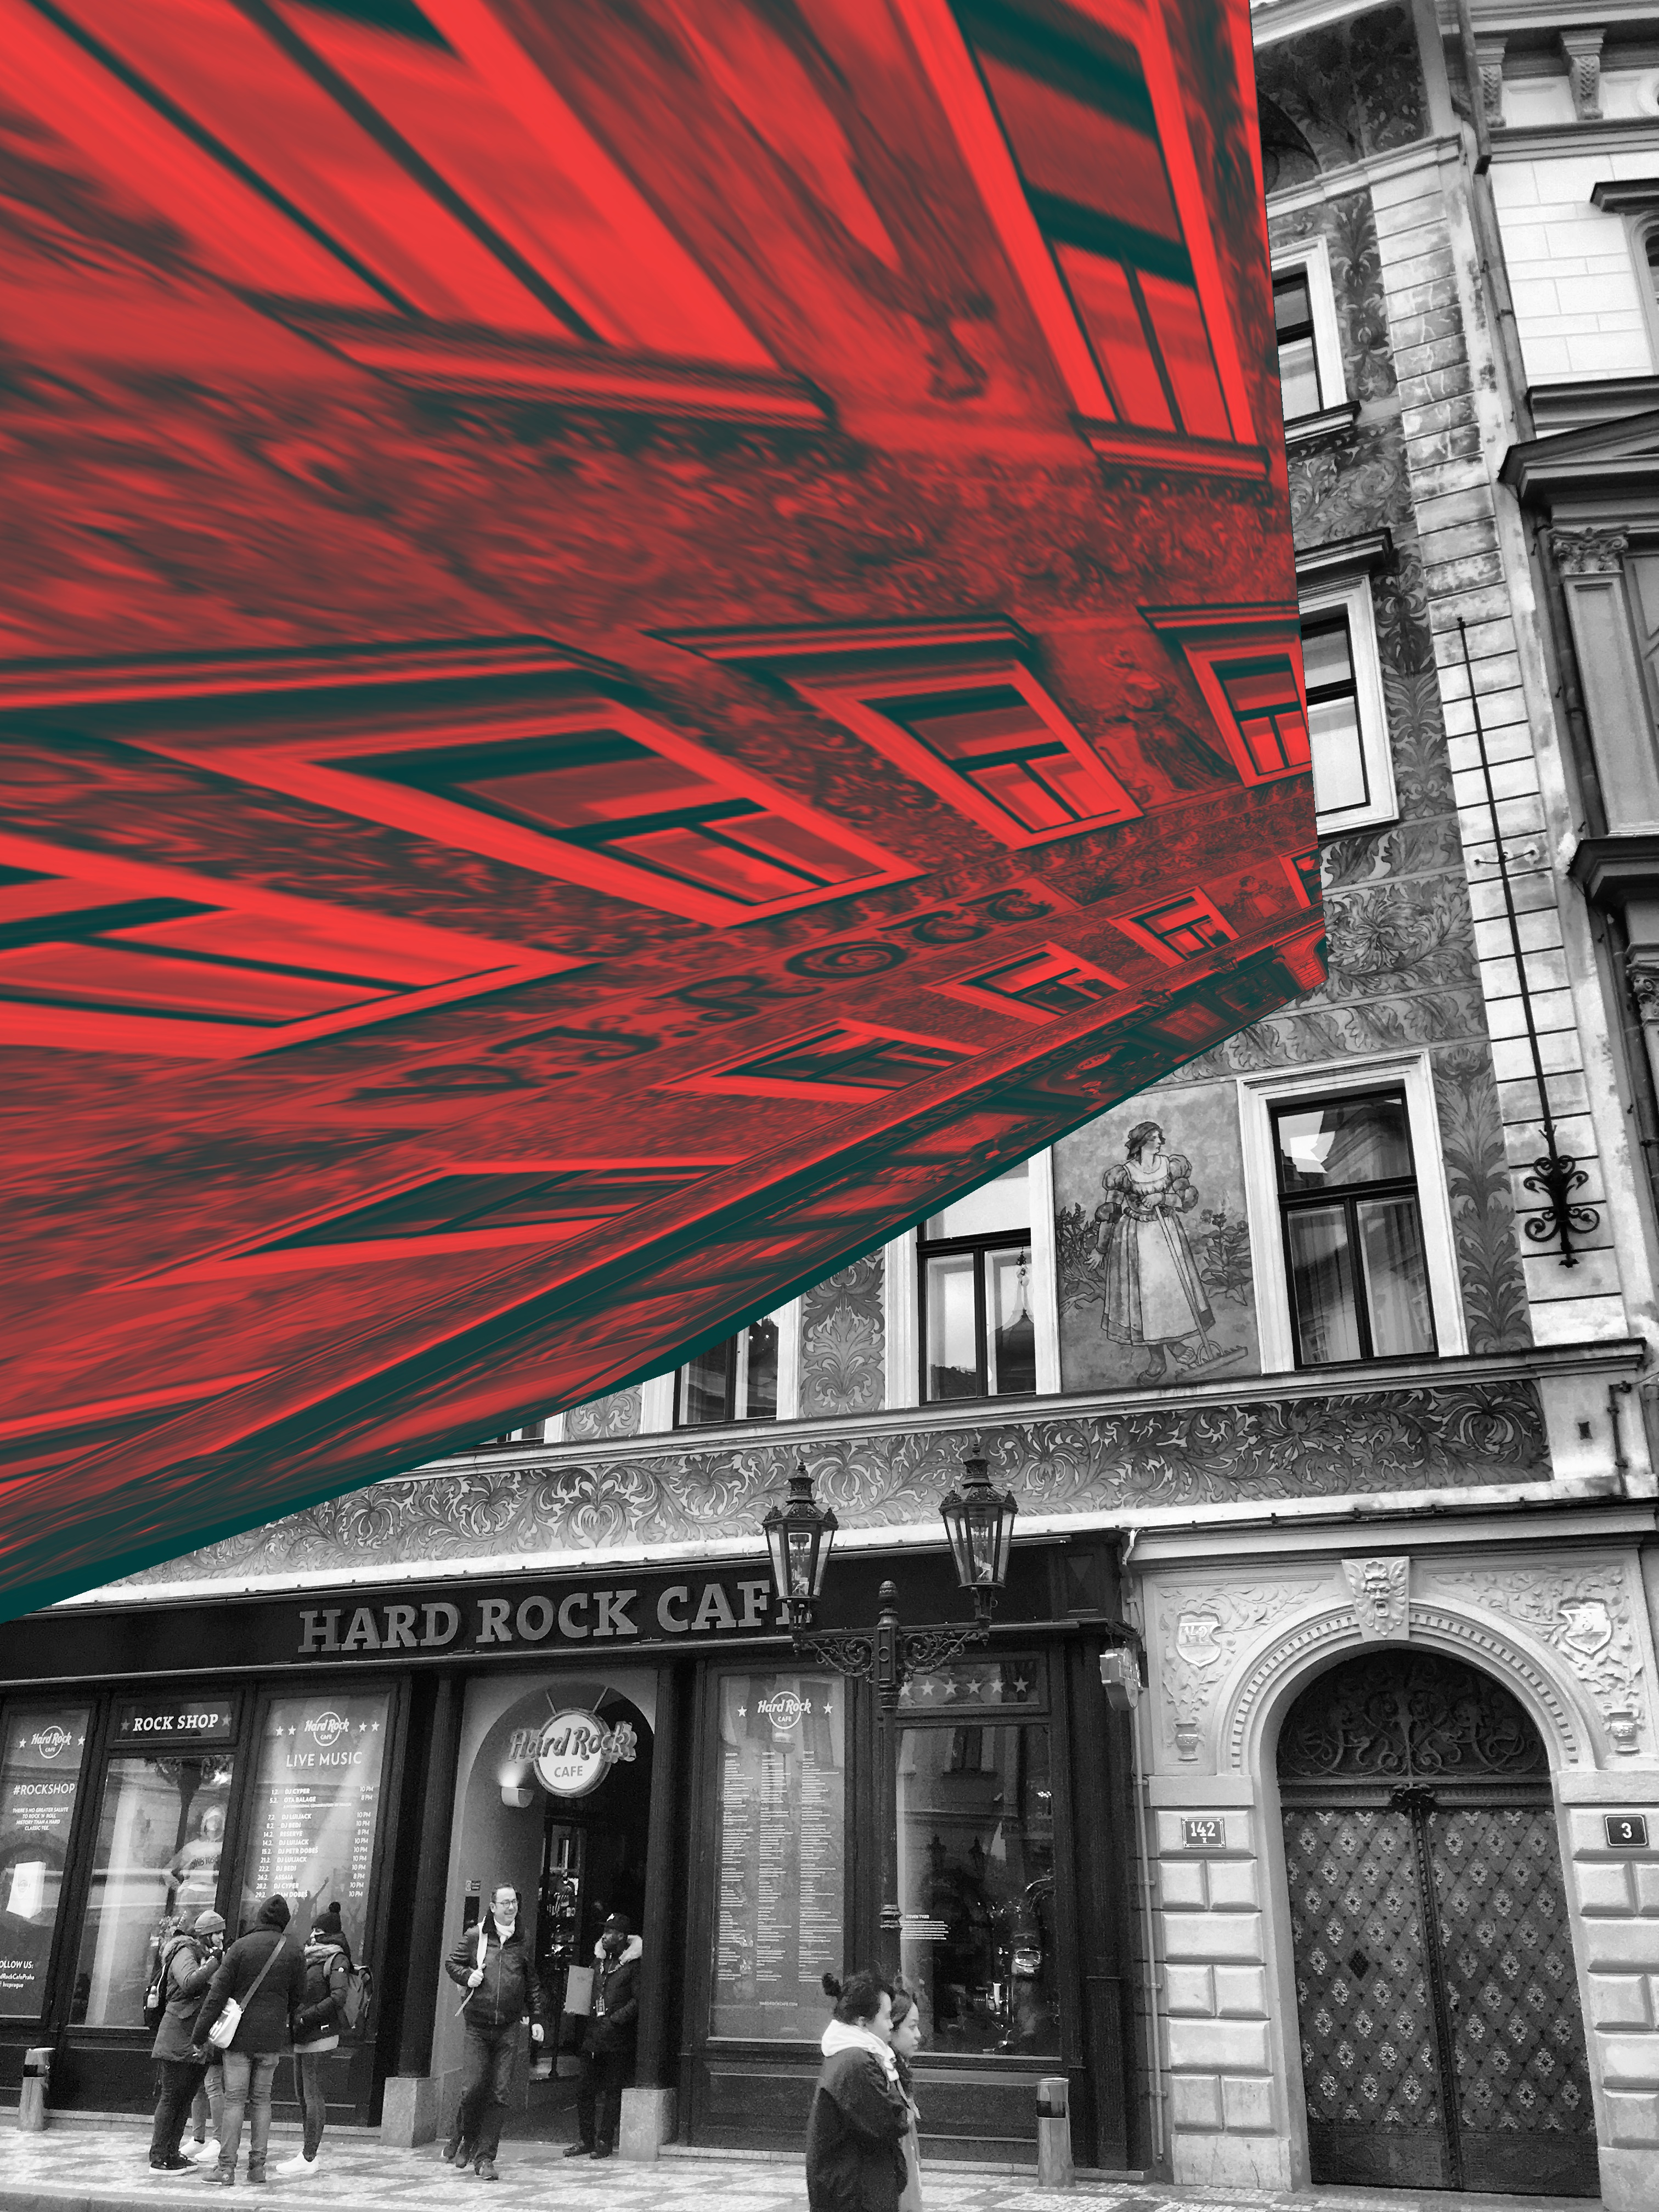
\includegraphics[width = 0.39\linewidth] {pictures/ORB_BEBLID_BF_3_img1.jpg}
                    \caption[Early evaluation of our prototype.]{Early evaluation of our prototype. Correctly displayed object (building) in the scene on the left and badly displayed on the right. Building photos are from Jan Šefčík's image database~\cite{Sefcik2020}.}
                    \label{fig:featureMatchingYesNo}
                \end{figure}
                
                \subsubsection*{Test results}
                The test results can be seen in the table~\ref{table:featureSpeedComparison}. In case of the SIFT-SIFT and SIFT-RootSIFT columns, two different values can be explained in the following way. The feature interface offers to detect and describe features in one step (values outside brackets), or to split the calculation to two steps (values in brackets). In the case of SIFT, the splitting into two calculations leads to a significant speed decrease. We think this behavior is specific to the OpenCV SIFT implementation.
                
                The conclusion from this testing is that SIFT is by a magnitude order slower than ORB. The RootSIFT modification is only 5\% slower than SIFT and is more successful. Also the combination of SIFT feature detection and BEBLID description has 100\% success rate (in our test), the same as RootSIFT and it is only slightly slower than SIFT-SIFT. Method combinations with ORB ended up as less successful in terms of correct results than combinations with SIFT. But on the other side, they are multiple times faster. The combination of ORB and BEBLID achieves even a 35\% increase in speed in comparison to pure ORB and still maintains the same success rate.

\begin{table}[]
\centering
\resizebox{\linewidth}{!}{
\begin{tabular}{|l|c|c|c|c|c|}
\hline
\begin{tabular}[c]{@{}l@{}}Detection:\\ Description:\end{tabular} &
  \multicolumn{1}{l|}{\begin{tabular}[c]{@{}l@{}}SIFT\\ SIFT \end{tabular}} &
  \multicolumn{1}{l|}{\begin{tabular}[c]{@{}l@{}}SIFT\\ RootSIFT \end{tabular}} &
  \multicolumn{1}{l|}{\begin{tabular}[c]{@{}l@{}}SIFT\\ BEBLID \end{tabular}} &
  \multicolumn{1}{l|}{\begin{tabular}[c]{@{}l@{}}ORB\\ ORB\end{tabular}} &
  \multicolumn{1}{l|}{\begin{tabular}[c]{@{}l@{}}ORB\\ BEBLID \end{tabular}} \\ \hline
1 success     & yes           & yes   & yes   & yes  & yes  \\ \hline
1 time (ms)   & 7758 (13775)  & 8064 (13543) & 7729  & 1361 & 897  \\ \hline
2 success     & yes           & yes   & yes   & yes  & yes  \\ \hline
2 time (ms)   & 10025 (17958) & 10220 (17824) & 9931  & 1626 & 1022 \\ \hline
3 success     & no            & yes   & yes   & no   & no   \\ \hline
3 time (ms)   & 9843 (17706)  & 10556 (17940) & 10120 & 1700 & 1086 \\ \hline
4 success     & yes           & yes   & yes   & yes  & yes  \\ \hline
4 time (ms)   & 7608 (13687)  & 8274 (13639) & 7794  & 1395 & 916  \\ \hline
5 success     & yes           & yes   & yes   & yes  & yes  \\ \hline
5 time (ms)   & 7739 (13500)  & 8203 (13903) & 7636  & 1349 & 882  \\ \hline
Total success & 4/5           & 5/5   & 5/5   & 4/5  & 4/5  \\ \hline
Average time  & 8595 (15325)  & 9063 (15370) & 8642  & 1486 & 961  \\ \hline
\end{tabular}
}
\caption[Comparison of OpenCV feature detection and description methods]{Comparison of OpenCV feature detection and description methods. All tests included processing of 48 images with the limit of detected features set to 1000. There are two values for SIFT-SIFT and SIFT-RootSIFT columns, because time depends on the usage of the OpenCV methods.}
\label{table:featureSpeedComparison}
\end{table}
                
                
                %can be done
                %what methods are implemented
            \subsection{Feature matching}
                In Šefčík's work~\cite{Sefcik2020}, it is stated that another option is to use matching methods based on FLANN. The advantage of these methods is that it creates data structures which speeds up the searching of a match for the feature. But these structures have some additional costs, such as the cost of the structure built at the beginning. The number of features has to be therefore large enough, so the FLANN based matching is faster than the brute-force matching. The question is which method is faster in our case.
            
            \subsection{Feature matching in OpenCV}
                Both of the above mentioned matching methods are implemented in OpenCV. We therefore prepared a test, similar to that one mentioned above, to find out which matching method is the fastest in our case. We were interested in how the matching methods performed, according to the used distance to compare the descriptors.
            
                The test result can be seen in the table~\ref{table:matcherSpeedComparison}. We can see that the brute-force matching is clearly faster than the FLANN-based matching. The number of features is the key in which method is faster. So we also performed a test without maximum detected feature limit (it led to about 5000 features per image) and this test also favoured brute-force matching. The type of distance used influences the matching time as well. Hamming distance made both matching methods to run faster than L2 norm (Euclidean) distance. Based on this test we could consider to use only brute-force matching. In case of change for another matching it would not be a problem because all OpenCV feature matching implement the same interface.
                
\begin{table}[]
\centering
\begin{tabular}{|l|c|c|c|c|}
\hline
\begin{tabular}[c]{@{}l@{}}Distance:\\ Matching method:\end{tabular} &
  \multicolumn{1}{l|}{\begin{tabular}[c]{@{}l@{}}Hamming\\ Brute force\end{tabular}} &
  \multicolumn{1}{l|}{\begin{tabular}[c]{@{}l@{}}Hamming\\ FLANN\end{tabular}} &
  \multicolumn{1}{l|}{\begin{tabular}[c]{@{}l@{}}L2 norm\\ Brute Force\end{tabular}} &
  \multicolumn{1}{l|}{\begin{tabular}[c]{@{}l@{}}L2 norm\\ FLANN\end{tabular}} \\ \hline
1 success         & yes & yes & yes & yes \\ \hline
1 time (ms)       & 86  & 531 & 119 & 898 \\ \hline
2 success         & yes & yes & yes & yes \\ \hline
2 time (ms)       & 91  & 539 & 121 & 922 \\ \hline
3 success         & no  & no  & no  & no  \\ \hline
3 time (ms)       & 87  & 584 & 119 & 915 \\ \hline
4 success         & yes & yes & yes & yes \\ \hline
4 time (ms)       & 88  & 541 & 120 & 921 \\ \hline
5 success         & yes & yes & yes & yes \\ \hline
5 time (ms)       & 90  & 526 & 123 & 902 \\ \hline
Total success     & 4/5 & 4/5 & 4/5 & 4/5 \\ \hline
Average time (ms) & 88  & 544 & 120 & 912 \\ \hline
\end{tabular}
\caption[Comparison of two matching methods.]{Comparison of two matching methods. All tests included processing of 48 images with the limit of detected features set to 1000.}
\label{table:matcherSpeedComparison}
\end{table}
        
\chapter{Prototype development}
    As a main part of our work is the creation of a prototype, which is intended to be a development, debugging, and testing platform for a localisation solution. Such a prototype would be similar to that one that was developed in Jan Šefčík’s work~\cite{Sefcik2020}. The goal of doing this is to push what Šefčík has done further and to extend the process by calculating not only the transformation matrix between the reference image space and the image space of the image queried to be recognised.
    
    \section{Design}
        We will follow the design of Jan Šefčík\cite{Sefcik2020}. So in this section, we will describe the changes from the Šefčík's design that we will make.
        
        \subsection{Programming language}
        The main change is that we will choose C++ programming language instead of Python. To be able to work with a file system and parse JSON files we decided to use Boost (set of C++ libraries).
        
        C++ will be used, because of its efficiency and the code itself will be more similar to that one in the application localisation module. The C++ is planned as a programming language for the computation parts in the localisation modules. We expect that in that way it will be possible to integrate big code parts from our prototype.
 
        \subsection{Configurability}
        We will continue using JSON files for storing additional image data. However we plan to create a more sophisticated configuration system than Šefčík’s, where the initial configuration Python source files were used. That is not possible in C++ without compiling. We want to approach it in a more user-friendly way by moving the configuration into JSON files. This configuration will be divided into more JSON files, so they can be easily exchanged. They will be all linked in main JSON configuration file that will have following form:
        \begin{minted}{json}
{
    "reference_images" : "filepath/references.json",
    "scene_images" : "filepath/scenes.json",
    "parameters" : "filepath/parameters.json",
    "output_root" : "Where/to/save/output/",
    "run_name" : "some name"
}
        \end{minted}
        The \texttt{reference\_images} field will point to JSON with file paths to the reference images of buildings and in a similar way for other fields. The JSON file with parameters will be a file with parameter fields similar to that mentioned above. Based on our testing of feature detecting and extracting methods we observed that the configuration data changing the most across tests is the input scene image. The JSON file with scene images file paths will have following structure allowing smooth workflow:
        
        \begin{minted}{json}
{
"index" : 0,
"scene_images" : [
                 "filepath/scene1.jpg",
                 "filepath/scene2.jpg"
                 ]
}
        \end{minted}
        where the \texttt{index} determines the used scene from the \texttt{scene\_images} array. The most frequent expected use case is including going through the scene images and in this case it is needed to increment the index only.
        
        \subsection{Database}
        Same as in Šefčík's work we will use a file-system database to store images. All the needed image data other than the image itself will be stored in JSON files within the same directory as the images and the same name but the suffix. Information about reference images of buildings will contain localisation data and information about the scene images will be the camera intrinsic parameters and eventually the global position, where the image was taken.
        
        The file paths of the images will be stored in a dedicated JSON file. To fill our database with images we will use image sets created by us and the images from the work of Tatiana Popova~\cite{Popova2021}.
        
        \subsection{Output}
        The current mobile application DTBQ interface for localisation modules requires global coordinates and rotation to the object in the form of a quaternion, so that will be realised as well. Beside this, the prototype will calculate a 3D transformation from the world space to the local space of the camera.

        The result will be provided in the form of image visualisation and text information. Both will be provided in the real-time while running the prototype or by saving the output into files. This will create the options to debug the application and also create and store test results. The text information will include the information about the processing and the result.
        
        \subsection{Elimination based on location}
        An elimination of images based solely on global coordinates will not be a part of our prototype. The intention of the prototype is to test the algorithms and methods and create the solution for given problems. The location elimination would significantly decrease the input to these methods.

    \section{Implementation}
        In this section we write about the realisation of the localisation prototype. In this section we first describe what inputs have been defined and which outputs have to be expected. We then explain what processing is done to calculate the output from the input.

        \subsection{Input and output formats}\label{sec:InputOutputFormats}
            In this part we describe the necessary inputs and expected outputs of our localisation prototype. We expect that our localisation prototype will be similar to other possible localisation solutions in the DTBG project. So this information could be used in further development in the DTBQ project.

            \subsubsection*{Reference building images}
                The input images on the side of buildings with known locations to be recognized in the camera scene are called reference images. Such an image of a building has to be created in a way that it looks like a parallel projection from the front of a building. The image has to be without the perspective deformation as seen in the image~\ref{fig:testRefImageIllustration}. In this illustration is visible how the reference image was created. The perspective is removed so the real world horizontals are horizontal also in the image and the same for the vertical direction. In this way, the deformation is only partially removed, because the original image from which the image in the database was created is influenced by the perspective, that is well visible in the middle picture in the figure~\ref{fig:testRefImageIllustration}. A photo that was taken straight in front of the object/building from a large distance is ideal for creating the image for the database.
                
                \begin{figure}
                    \centering
                    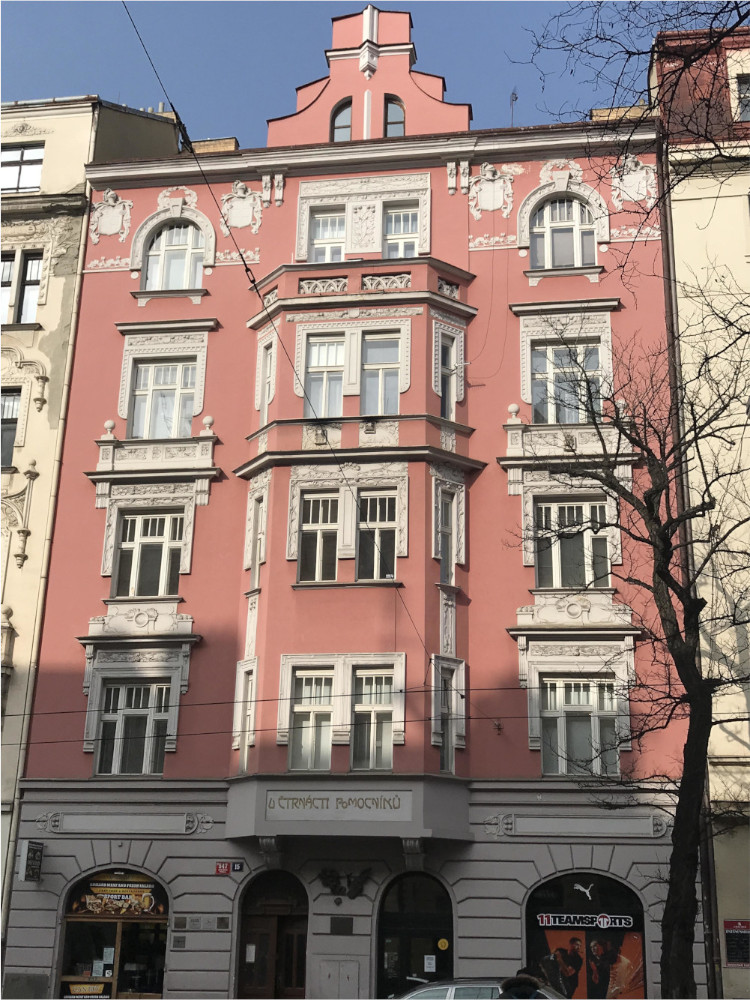
\includegraphics[width = 0.25\linewidth, height = 0.33\linewidth] {pictures/realisation/_building20_photo2.JPG}
                    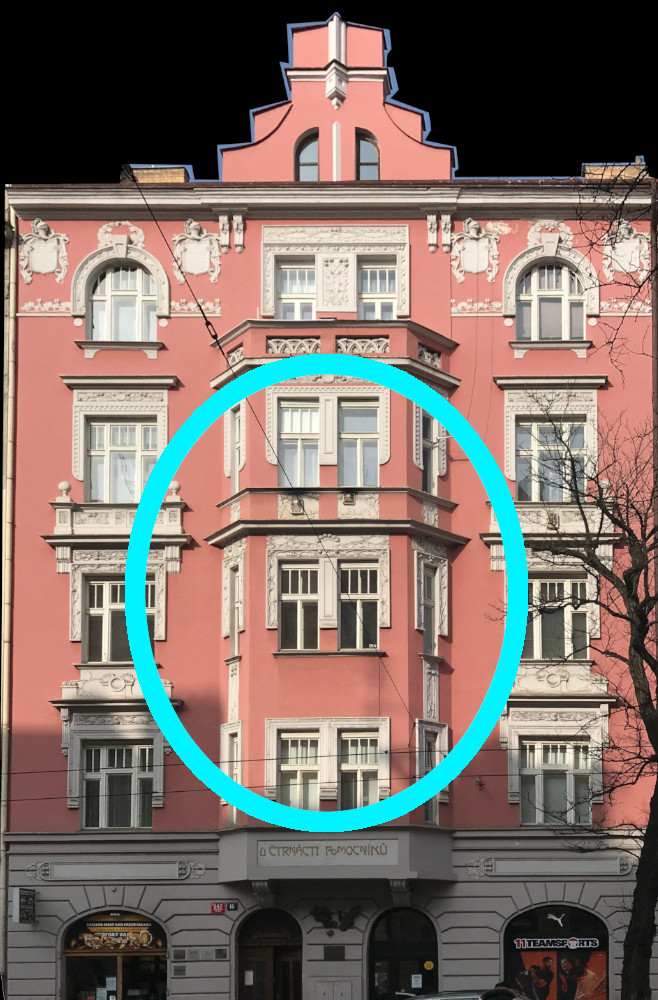
\includegraphics[width = 0.25\linewidth, height = 0.33\linewidth] {pictures/realisation/perspectiveCorrectionIllustration.jpg}
                    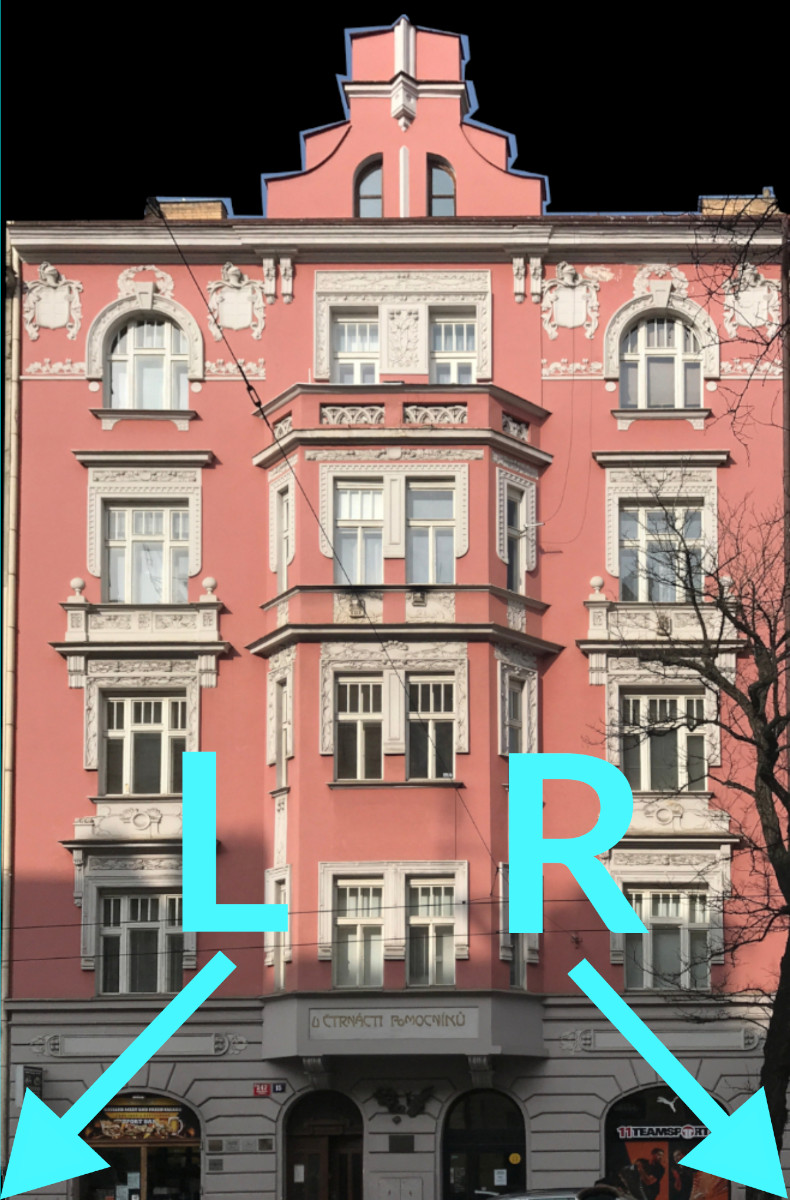
\includegraphics[width = 0.25\linewidth, height = 0.33\linewidth] {pictures/realisation/GCS_loc_requirements.jpg}
                    \caption[Illustration of creating a reference building image]{Illustration of creating a reference building image. On the left is the original picture, in the middle is the created database reference image. The cyan ellipse shows the remaining perspective deformation (the right side of the building extension is wider in the image than the left side). On the right is an illustration of the global location requirements. Original photo: Tatiana Popova}
                    \label{fig:testRefImageIllustration}
                \end{figure}
                
                With the reference building images, the \textit{JSON} files have to be created, with the same name and information about global coordinates (often just called GPS) of the left and right corner as in the right image in the figure~\ref{fig:testRefImageIllustration}. The position data has to be given exactly for the places in the left and right corner of the image, the lowest to the ground as possible. The JSON data structure looks like as follows:
                
                \begin{minted}{json}
{
    "right_corner": {
        "longitude": 14.419302807,
        "latitude": 50.086761105
    },
    "left_corner": {
        "longitude": 14.41927048,
        "latitude": 50.086600324
    }
}
                \end{minted}
                
            \subsubsection*{Camera scene images}
                Camera scene images are images taken by phone that are to be recognised. There are two following necessary requirements that has to be met to obtain valid results:
                \begin{itemize}
                    \item The scene image must not be cropped (it can be uniformly scaled).
                    \item The following information about the camera from which the images have been taken:
                    \begin{itemize}
                        \item Focal length,
                        \item The size of the camera sensor in both directions.
                    \end{itemize}
                \end{itemize}
                
                The following JSON content is example of a file attached to every scene image:
                \begin{minted}{json}
{
    "camera_name" : "Xiaomi Redmi 5 Plus",
    "focal_length" : 4,
    "sensor_size_x" : 4.96,
    "sensor_size_y" : 3.72
}
                \end{minted}
                
                The following sentences are guidelines for best results. The localisation has better results, if the scene image has such a resolution that the resolution of the building in the scene image matches the resolution of the reference building. This is usually slightly higher than a reference image resolution. A scene image is better recognised if taken parallel to the ground (rotated images might not work as well).
                
            \subsubsection*{Resolution of the images}
                The size of the image affects the computation time and size of allocated memory for the feature detection and extraction. When we used high resolution (\(\geq\) 12 MP) the size of used memory was about 3 GB at the peak. The resolution about 750x1000 (0.75 MP) works for us as a good compromise, because about 240 MB is allocated at the peak and the computation time is shorter.
            
            \subsubsection*{Global location }
                The global location in the global coordination system and rotation towards the object/building are the first possible result of the localisation. They are in the following format:
                \begin{itemize}
                    \item Global location of the camera defined as follows:
                    \begin{itemize}
                        \item Latitude in degrees,
                        \item Longitude in degrees.
                    \end{itemize}
                    \item Quaternion representing rotation of the direction vector pointing towards the detected object from the east.
                \end{itemize}
            
            \subsubsection*{Rotation-translation matrix}

                The second type of output is a rotation-translation matrix, which transforms points from world space to the local camera space, the same matrix that was described in section~\ref{sec:rotTransMat}. The biggest advantage of this output is that it does not depend on the global location. The output structure is following in this case:
                \begin{itemize}
                    \item Which object is in the scene image,
                    \item Rotation-translation matrix.
                \end{itemize}
                The global location of the left \(L\) and right \(R\) corner are exchanged in runtime (not in files) for the world space coordinates (virtual world space) which are defined as follows:
                \begin{equation}
                    L = (0, h, 1, 1)^T, \enspace
                    R = (w, h, 1, 1)^T
                    \label{eq:3DImagePlaneCorners}
                \end{equation}
                where \(w\) is the width and \(h\) is the height of the reference image.
                
        \subsection{Processing pipeline}
            In this section, we closer specify the processing pipeline. The whole processing pipeline is documented in the activity diagram in figure~\ref{fig:Activitiesdiagram}. Some parts are very similar to the activity diagram by Šefčík~\cite{Sefcik2020} in figure~\ref{img:sefcikDiagramAktivit}. We redone all these parts, but we followed similar principles, so we do not explain these parts, but we explain what we have added. Above all, we have added the possibility of pipeline configuration, calculation of 3D transformation, global localisation, and interpreting of the matching data.
            
            \begin{figure}
                \centering
                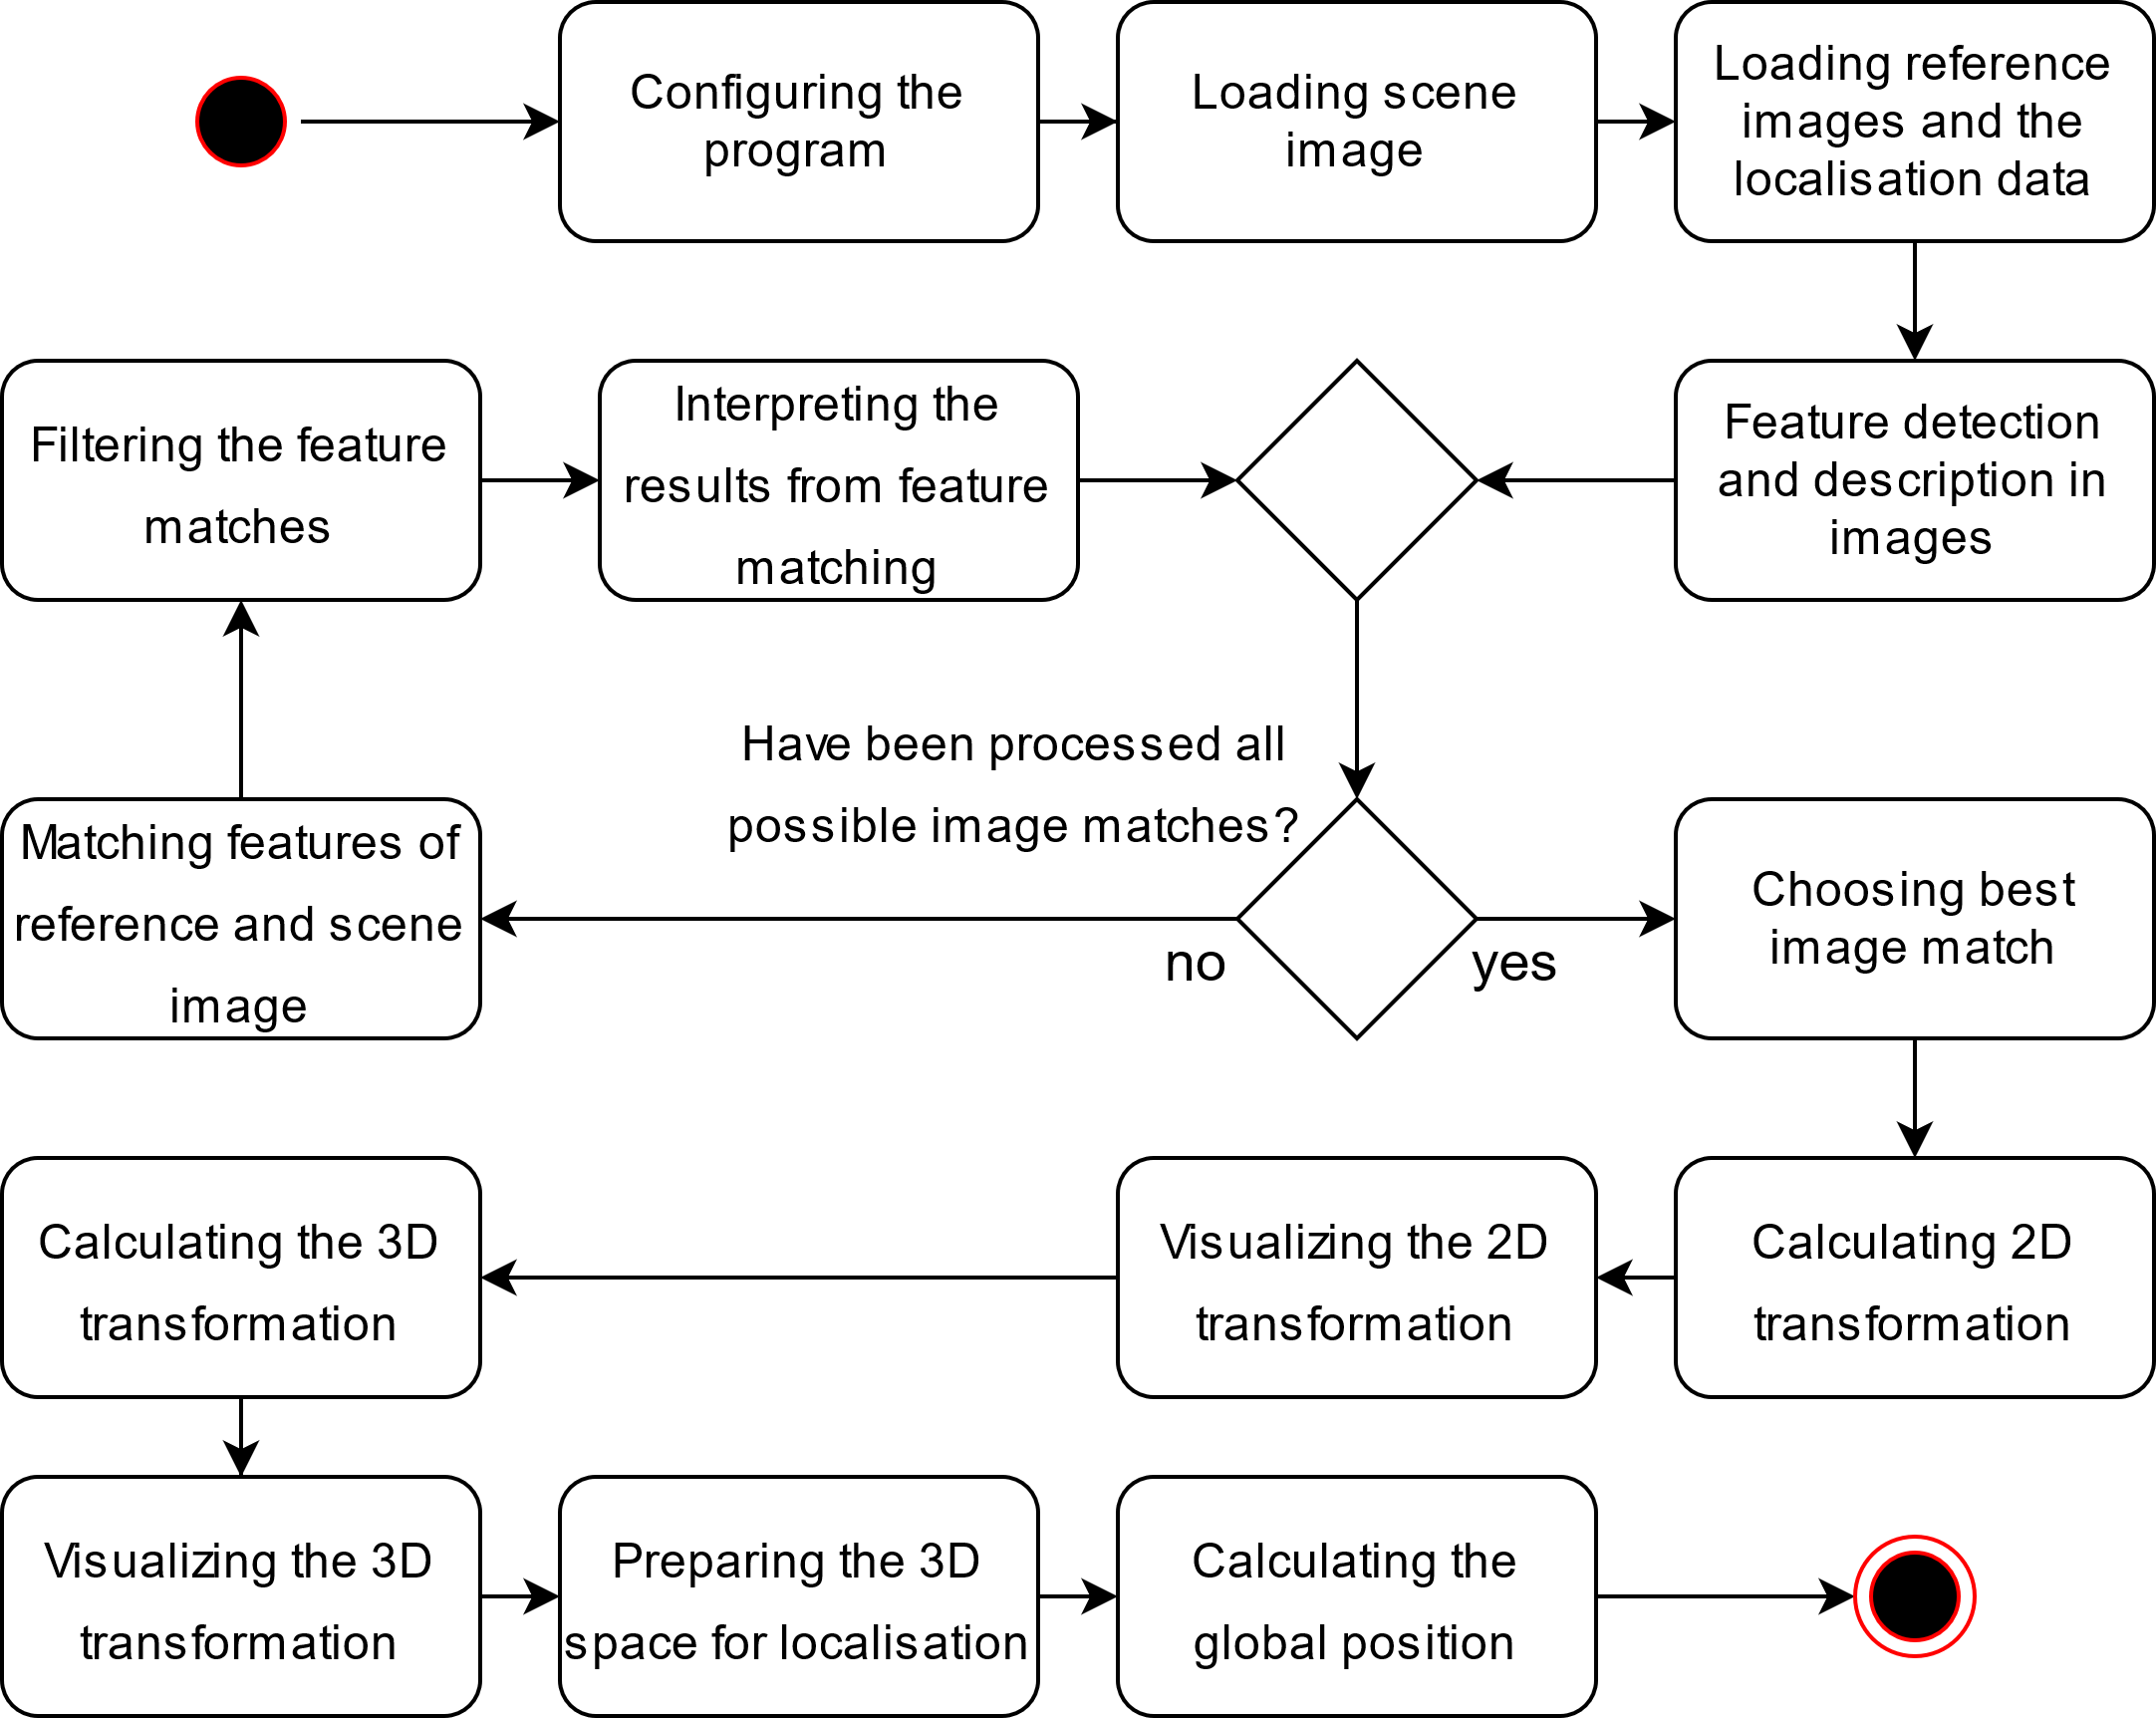
\includegraphics[width = 0.9\linewidth] {pictures/realisation/ourActivitiesDiagram.png}
                \caption{Activities diagram of our prototype for default configuration}
                \label{fig:Activitiesdiagram}
            \end{figure}
            
            \subsubsection*{Choosing the best match}
                During the development of the prototype, we searched for the best option for how to choose the correct match between multiple matches. We found three viable options, namely the average of values from the Lowe's ratio test, the average distance of feature matches and the ratio between matches and filtered feature matches. We discovered strong positive correlation between these three values. We chose the way of searching for the highest ratio between matches and filtered matches. It has an asymptotic complexity of \(O(1)\) in comparison to the linear asymptotic complexity of the averages depending on the number of matches.
                
            \subsubsection*{Calculation of 3D transformation}
                In this calculation, the PnP problem has to be solved and the rotation-translation matrix has to be found. We used the OpenCV iterative implementation of that problem in the OpenCV module \textit{calib3d}. As an input for this PnP problem solution we provide a 3D plane geometry (building facade) of the image and 2D projection of the reference image corners in the space of the scene image. These corners can be obtained by transforming the original reference corners with the transformation matrix from the 2D solution.
                
                The 3D plane geometry \(G\) for image of size \(h\times w\) is defined as follows:
                \begin{equation}
                   G = \{(0, 0, 1, 1)^T, \enspace (w, 0, 1, 1)^T, \enspace (w, h, 1, 1)^T, \enspace (0, h, 1, 1)^T\}.
                \end{equation}
                
            \subsubsection*{Localisation}
                When the corners location of the building plane (facade) are known in the camera space and the global coordinates are known for the two bottom corners of the building, we can calculated the global coordinates of the camera. For our prototype, we only considered a flat ground and the computation will be less accurate in the case of a slope along the building facade and inaccurate in case of a slope in different directions. But because the dowry towns are mostly on flat ground, it is not a significant problem.  
                
                There is one more problem and it is the height at which the camera of the phone is above the ground. It is similar to the problem with the hilly terrain, but it has an easier solution because we can expect some average phone holding height. For this problem, we created an illustration in the figure~\ref{fig:standingPersonProblem}. The problem is that the real location of the camera global coordinates are not at the origin (where is the camera located) but it lies on the intersection of ground and the real world up~vector passing through the origin. As seen in the image, there is a small distance between the intersection and y-axis which makes the difference.
                
                \begin{figure}
                    \centering
                    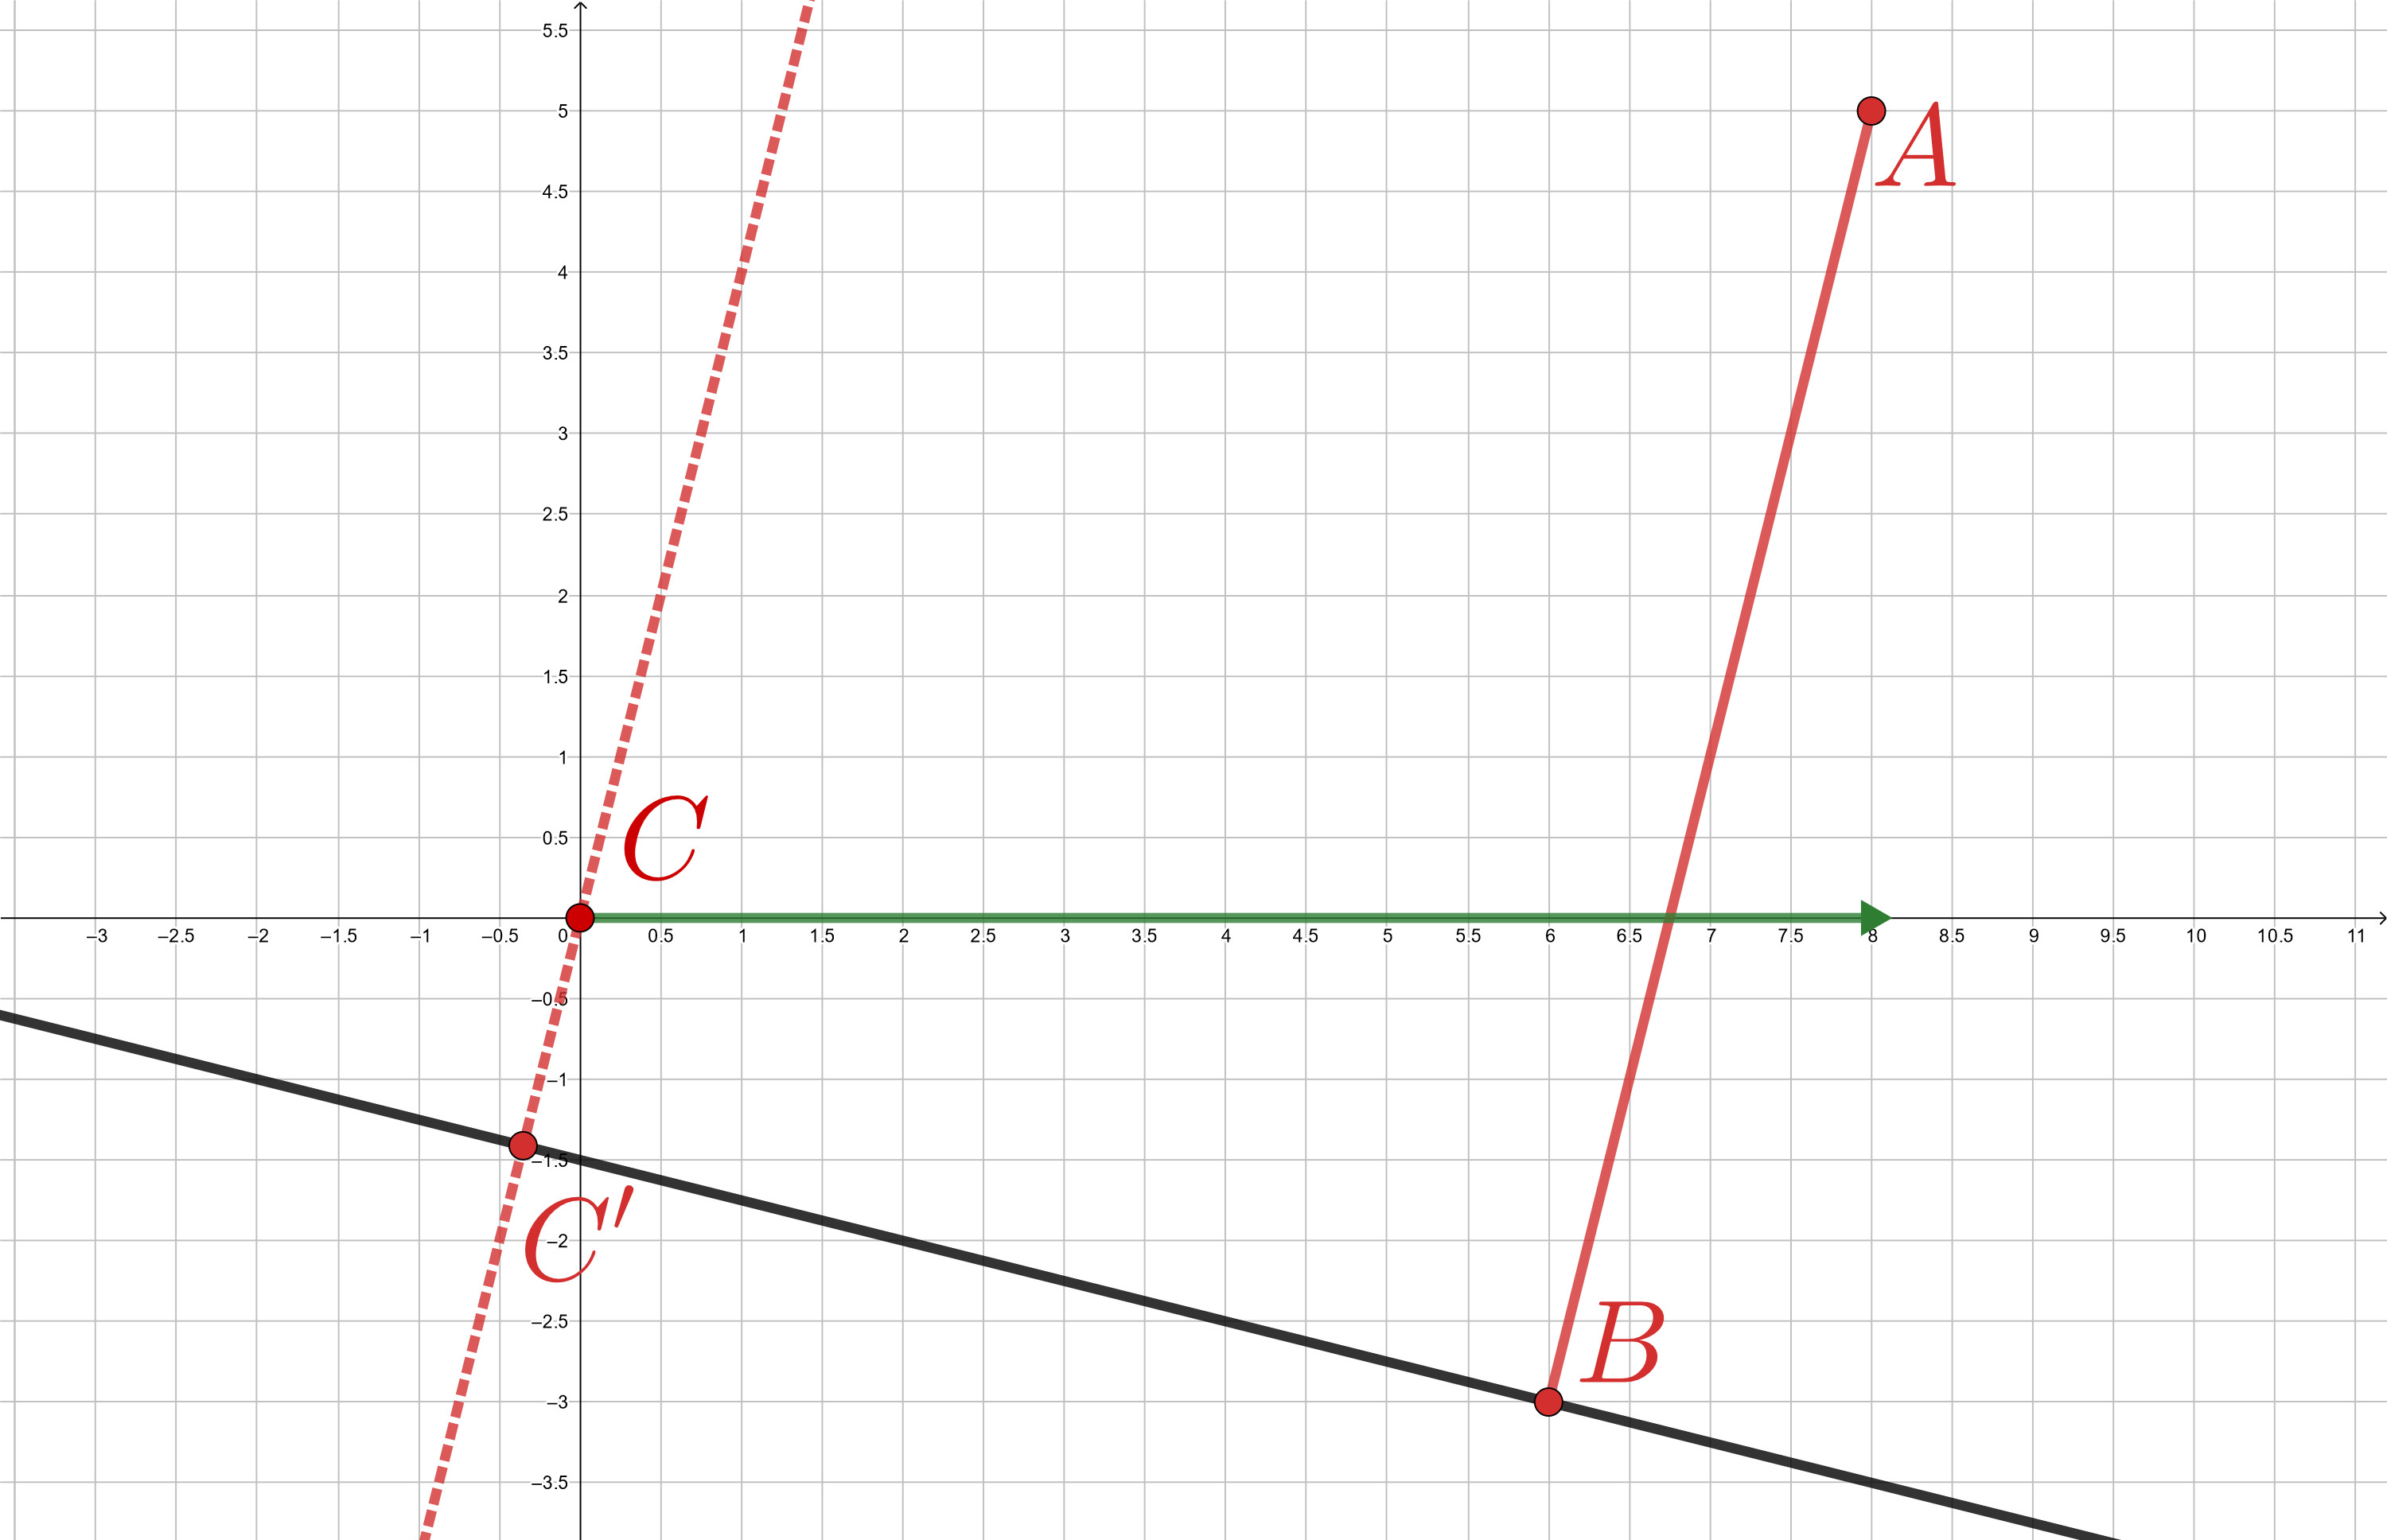
\includegraphics[width = 0.8\linewidth] {pictures/realisation/standingPersonProblem.jpg}
                    \caption[Illustration from side of a camera coordinates correction.]{Illustration from side of a camera coordinates correction. The green line stands for vector in the direction of the camera view, the black line stands for the ground, the red line then for building facade from the side, the red striped line is then real world up~vector in place of camera \(C\) and \(C'\) is a intersection of the up~vector and the ground.}
                    \label{fig:standingPersonProblem}
                \end{figure}
                
                The up~vector is computed from the building facade. Therefore, if it is not guaranteed that the facade of the building will create a real world up~vector (as in the case of objects other than buildings), we recommend turning off this feature in the configuration of our prototype.
                
        \subsection{Configurability}
            Our prototype was realised with the flexibility in mind. It is possible to configure which methods are used for feature detection, feature extraction, feature matching and possibility to configure these methods by adjusting the OpenCV parameters. List of these methods consists of SIFT, RootSIFT, BEBLID, ORB, brute-force matching and FLANN based matching. The Lowe's ratio is also possible to easily set in configuration. Other possible settings to disable or enable are global coordinates calculations, optimisation for bigger accuracy when measuring time and optimisation for calculation of the global location.
                
            The last configurable thing is if the log of the whole process with images is displayed in real-time or saved to files. The prototype creates a log with information about what it processed, how and with what results and values.
            
            All the parameters of the feature detection and extraction methods (except detected feature limit) are configurable only in the header file before compilation. They are in the header file, because they are determined to be changed only by a knowledgeable person. However the prototype is built so they can be changed without any problems.
                
    \section{Experimental evaluation}
        We have done testing in which we focused mainly on the comparison with the phone location sensor (GPS sensor). We did this because the use of the prototype (a future phone module) has to provide a more accurate location to that one that is provided by the phone sensors.
                
        \subsection{Methodology}
            We prepared a database of reference building (or other objects) images and then created a set of 25 tests. In each test, we queried images of the scenes. Some of the images were taken from the image database created by Tatiana Popova for her bachelor thesis~\cite{Popova2021}. We created the rest of the images to cover our needs for testing which could not be covered with images from Popova's database. We made the tests with the intention to create similar conditions to these ones that would be present when using the mobile application.
                
            \subsubsection*{Reference building images}
                There were prepared all the objects that covered a wide variety of objects, but most of the objects are buildings, because that is mainly what the prototype was optimised for. We chose buildings with different architectural styles. With our tests we covered the following areas:
                \begin{itemize}
                    \item Buildings with one front facade,
                    \item Corner buildings,
                    \item Towers,
                    \item Free-standing columns.
                \end{itemize}
                    
            \subsubsection*{Scene photos}
                The image with the scene is such an image containing the building/object that we put into the database. The style of every scene image is such that it could be taken by any tourist/anyone. This means that the image was taken by phone camera from such places where people usually move like pavements. In more detail, the tests were created in a way that they cover all the following areas:
                \begin{itemize}
                    \item Ideal camera shots from front of the building,
                    \item Camera Shots from angles up to 50\degree,
                    \item Different weather and lighting conditions,
                    \item More reference objects in the scene.
                \end{itemize}
            
            \subsubsection*{Used algorithms and methods}
                We decided to use SIFT without modification, because it was tested a lot during its existence and considered to be reliable and as a \textit{golden standard}. We needed reliability, because we also needed to test other parts and thus the whole prototype. But for any future testing, we encourage the testing of a combination of SIFT and BEBLID or RootSIFT modification of SIFT. The parameters of the SIFT algorithms were set to default values except for a number of features that were set to 1000. For feature matching, we used the brute force matching and Lowe's ratio test and RANSAC for filtering.
            
            \subsubsection*{Measuring results}
                We saw three ways on how to measure the results. The first is to compute the global location and project it on the map with the global location given by the phone sensors. With this, we were able to decide which one better suits the photo scene and as a score we measured the difference between a more accurate and a less accurate solution. So the result will be in form of a number measuring increase of accuracy in comparison to phone sensors (negative number in case of accuracy decrease in comparison to phone sensors).
                
                The second way is to binary decide if the building was correctly recognised. That means if it was recognised which object/building is in the photo scene.
                
                The last way is to evaluate the understood relative location to the object/building in the form of a projection matrix. With such a matrix, we could render into the scene image a wire frame of a prism. This prism represents the understanding of the spatial characteristics of the object/building by our prototype.
                
                
        \subsection{Results}    
                We created a representation of the results in the form of a histogram~\ref{fig:main_test_result}, where the results of the first measuring method can be seen. The results are in the form of gained accuracy in meters in comparison to the phone positioning sensors. We assign -56.58 (the additive inverse of the maximum positive difference) as a value to the failed cases (when our prototype failed to identify the building in a scene image) and we obtain an average accuracy increase of 0.98 meters. This result is a small gain in accuracy from the results of the mobile device sensor. If we omit all the failing cases, the average increase in accuracy is 11.94 meters. If we further omit the undecidable cases (cases when we could not tell if the phone was more accurate or our prototype), we obtain an average accuracy increase of 15.68 meters (higher value is better). Thus, for that measurement, we can conclude that there are cases where our computer vision localisation solution fails completely, but if it does not fail, it provides superior accuracy in comparison to the phone sensors. It is important to note that no front facing test (ideal conditions) has failed.

\begin{figure}
\centering
\begin{tikzpicture}
\begin{axis}[
    ybar,
    ymin=0,
    xlabel = {Difference in meters},
    ylabel={Number of occurrences},
    grid = both,
    width = 0.8\linewidth,
    legend pos = north west]
]
\addplot +[
    hist={
        bins=20,
        data min=-60,
        data max=60
    }   
] table [y index = 0] {./data/final_test_values.txt};
\end{axis}
\end{tikzpicture}
\caption[Testing results of the prototype]{Testing results of the prototype in the form of a histogram. The values in the histogram are the differences between the phone sensor's and our prototype's location output in meters. If the result was more accurate for our prototype, then the numbers are representing the accuracy increase compared to data provided by phone sensors. Special value is -56.58, this has been assigned to 4 cases where our prototype completely failed. Zero was assigned to 5 undecidable cases.}
\label{fig:main_test_result}
\end{figure}

                The second measurement results are 21 (84\%) successes and 4 (16\%) failures.
                
                The last measurement method has similar results as the previous methods, because when the object was recognised (success), then at least a somewhat accurate understanding of the spatial object/building characteristics was created. Usually such a result is the same or better than the image~\ref{subFig:somewhat_good}. The images in the figure~\ref{fig:prism_volume_matching} represent a perfect match and a fail. In the image with the fail was the volume of the column missed, but on the other side, in the successful image, the object is perfectly matched with the prism.
                
                \begin{figure}
                    \centering
                    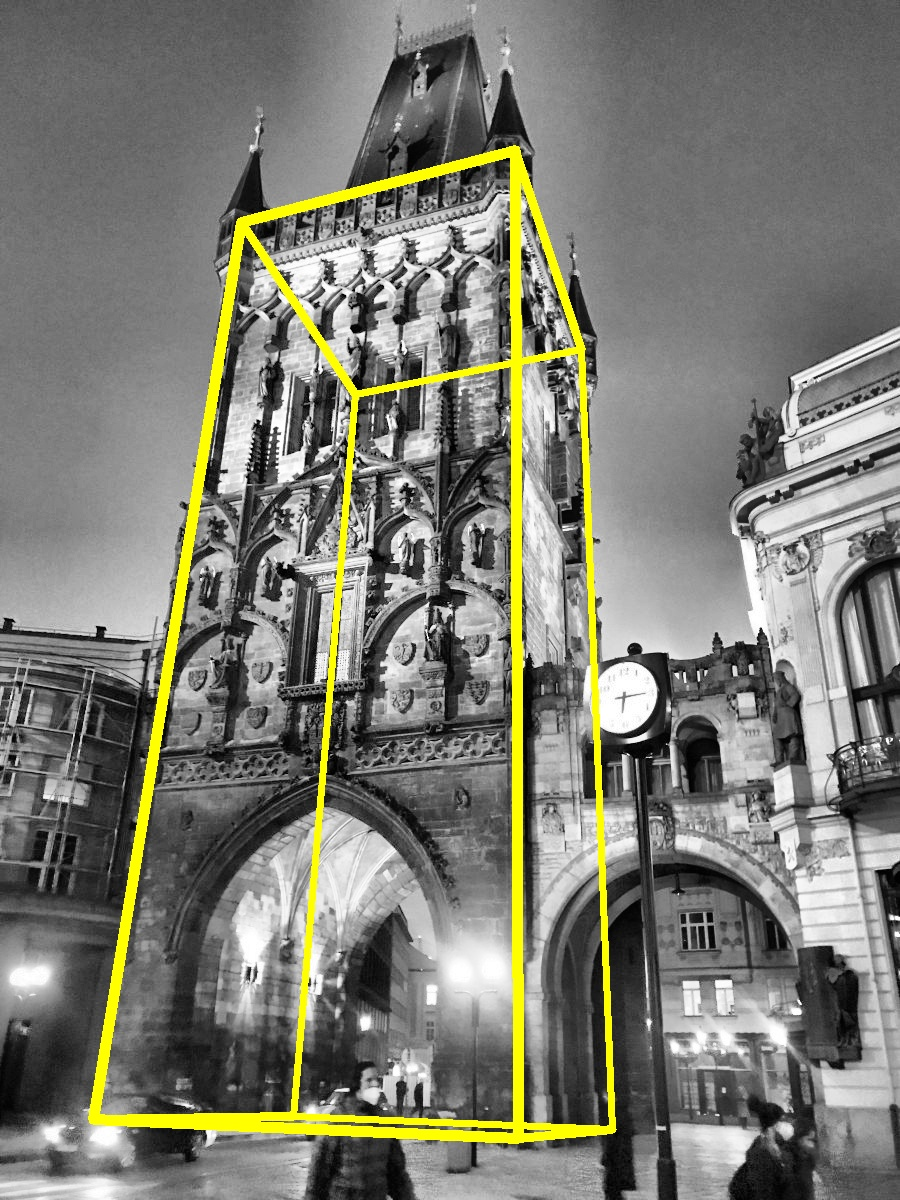
\includegraphics[width = 0.39\linewidth, height = 0.52\linewidth]{pictures/tests/illustration/best_result.jpg}
                    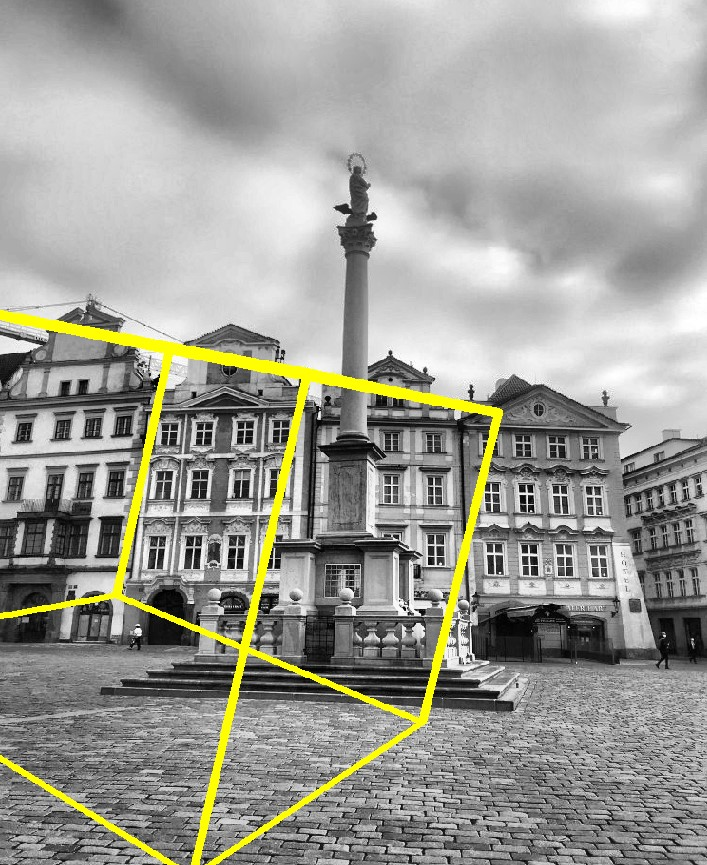
\includegraphics[width = 0.39\linewidth, height = 0.52\linewidth]{pictures/tests/illustration/fail.jpg}
                    \caption[Results of understanding of the spatial object/building characteristics]{Results of understanding of the spatial object/building characteristics. On the left is the best result, where the prism perfectly matches the tower. On the right is then a totally spatially misunderstood object (fail). Author of original photos: Tatiana Popova}
                    \label{fig:prism_volume_matching}
                \end{figure}
                
                \subsubsection*{Notes to testing}
                During the testing, we improved the reference pictures database by adding a night version of objects or improving the images. In all tested cases, the daily reference pictures led to failure when testing with the night scene image. But after adding the night reference image, the object was detected and in one case ideally matched as seen in perfect match in figure~\ref{fig:prism_volume_matching}. Improvement of the reference images is well seen in the set of pictures~\ref{fig:referenceSizeImportance}, where it is well visible that the correct size (height to width ratio) of the reference image is very important to get right for the accurate matching.
                
                \begin{figure}
                \centering
                \begin{subfigure}{0.39\linewidth}
                    \centering
                    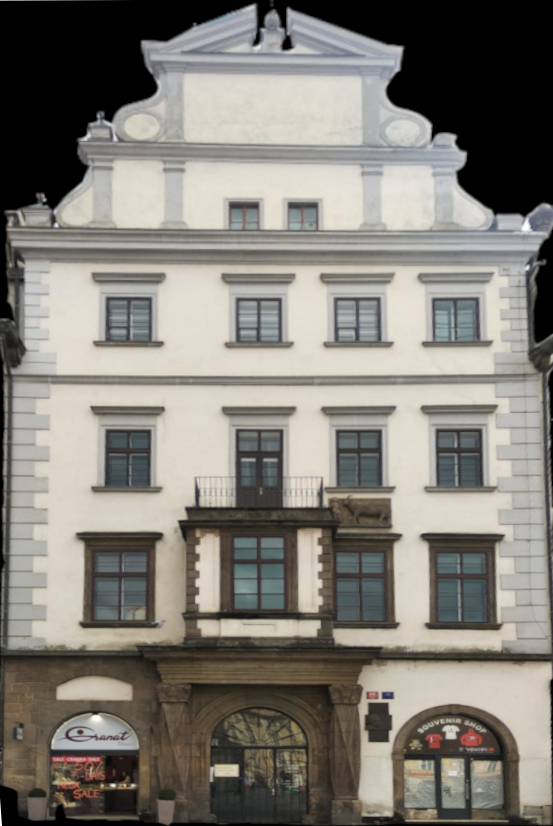
\includegraphics[
                        width=\linewidth]{pictures/tests/illustration/whiteHouse1ref.png}
                    \caption{Original reference}
                    \label{subFig:whiteHouse1ref}
                \end{subfigure}
                \begin{subfigure}{0.39\linewidth}
                    \centering
                    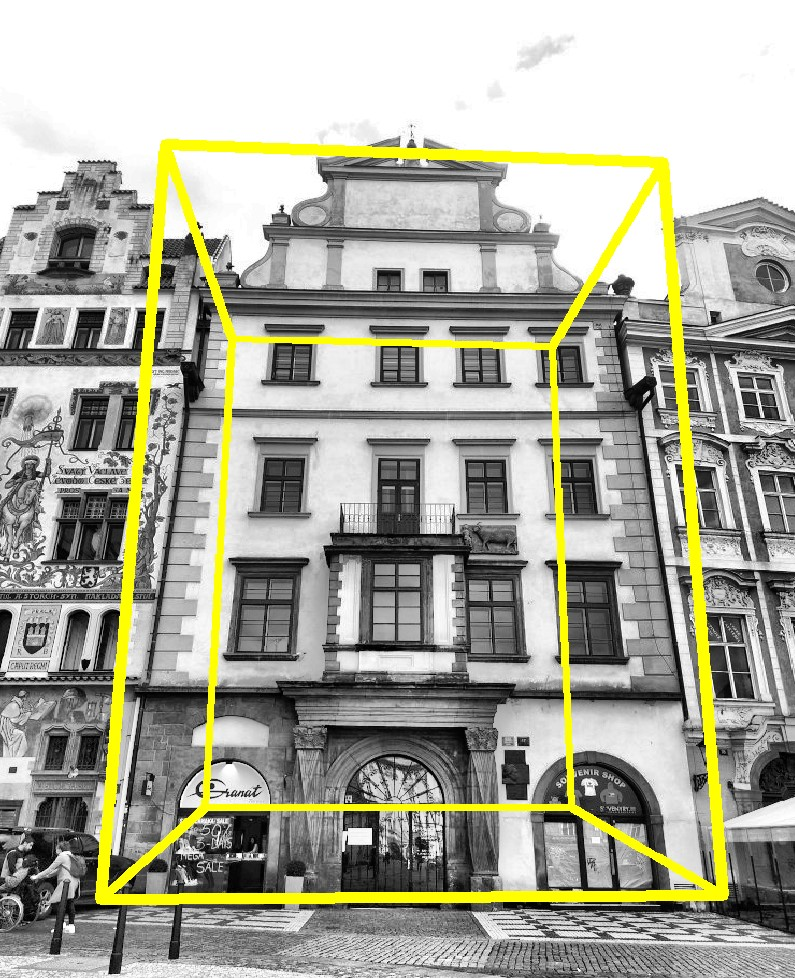
\includegraphics[
                        width=\linewidth]{pictures/tests/illustration/somewhat_good.jpg}
                    \caption{Result}
                    \label{subFig:somewhat_good}
                \end{subfigure}
                \\
                \begin{subfigure}{0.39\linewidth}
                    \centering
                    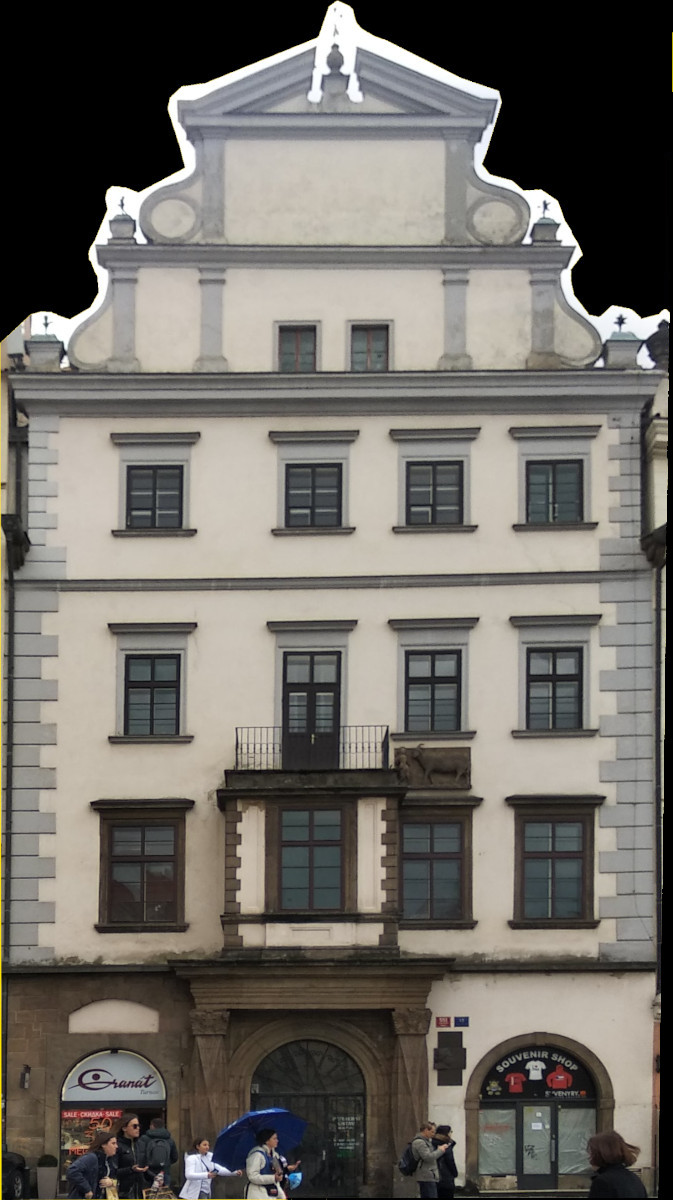
\includegraphics[
                        width=\linewidth]{pictures/tests/illustration/whiteHouse2ref.jpg}
                    \caption{Enhanced reference}
                    \label{subFig:whiteHouse2ref}
                \end{subfigure}
                \begin{subfigure}{0.39\linewidth}
                    \centering
                    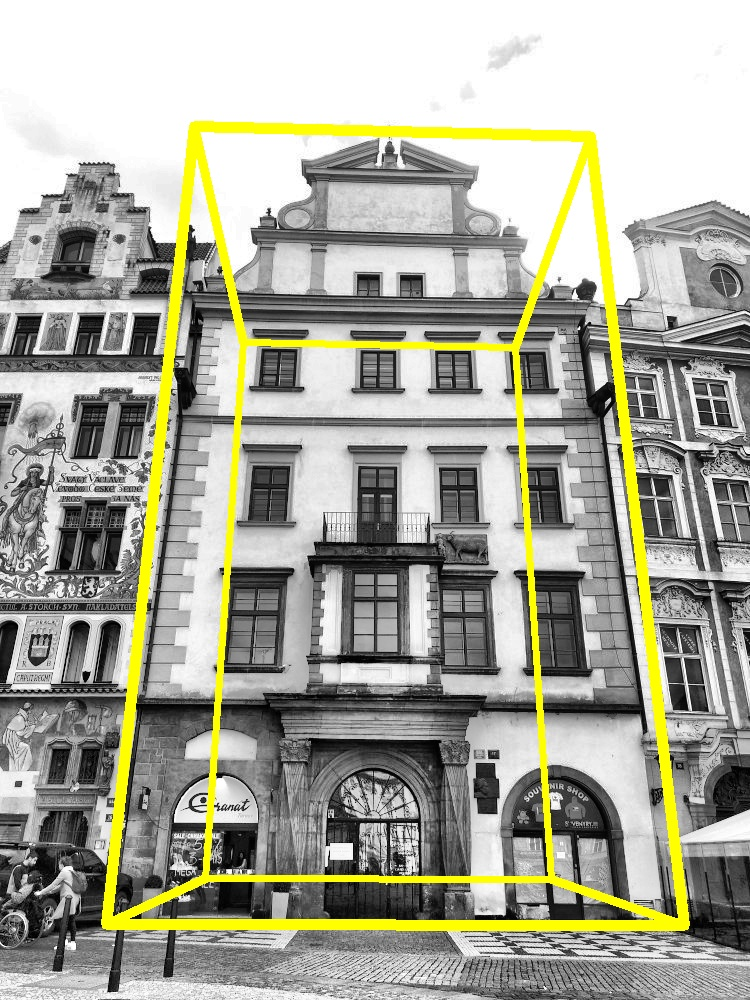
\includegraphics[
                        width=\linewidth]{pictures/tests/illustration/somewhat_better.jpg}
                    \caption{Enhanced result}
                    \label{subFig:somewhat_bette}
                \end{subfigure}
                \caption[Example of building's reference image size importance]{Example of building's reference image size importance. It is visible that the accuracy in the top result image is worse and it is visible that the reference picture is deformed (it is too wide). Photo: author}
                \label{fig:referenceSizeImportance}
            \end{figure}
                
                We tested a column at the town square where a building is visible in the background and we performed two tests with the same image. The first test was before and the second after adding the improved reference image. In the second test, the building in the background was detected instead of the column in the foreground. It is important to say that the first test failed. This case can be seen in the figure~\ref{fig:backgroundDetection}. Because of detecting the building in the background, the location was detected more accurately than from the phone sensors.
                
                \begin{figure}
                    \centering
                    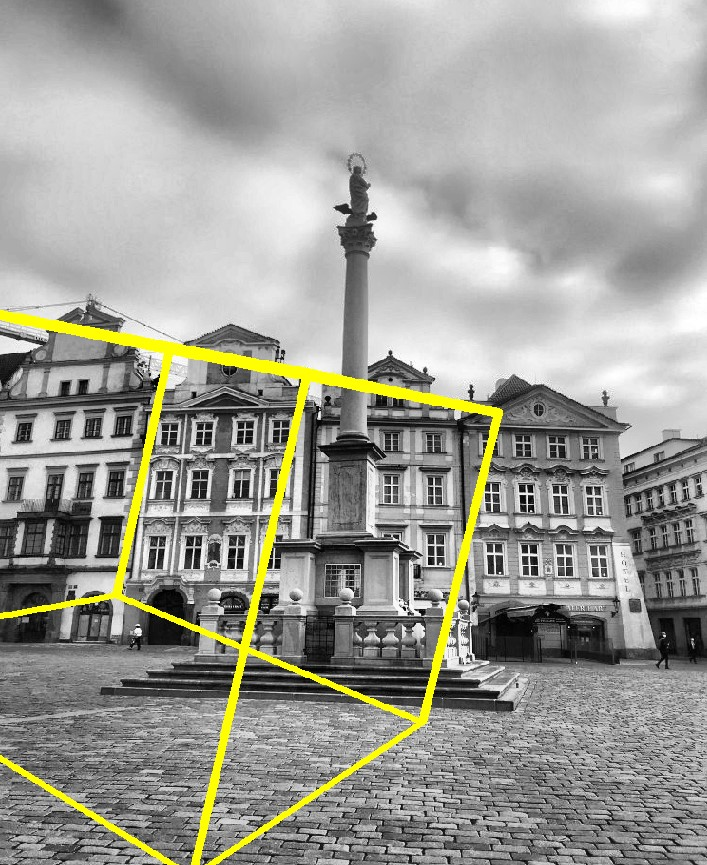
\includegraphics[width = 0.39\linewidth]{pictures/tests/1/sloup2_vol.jpg}
                    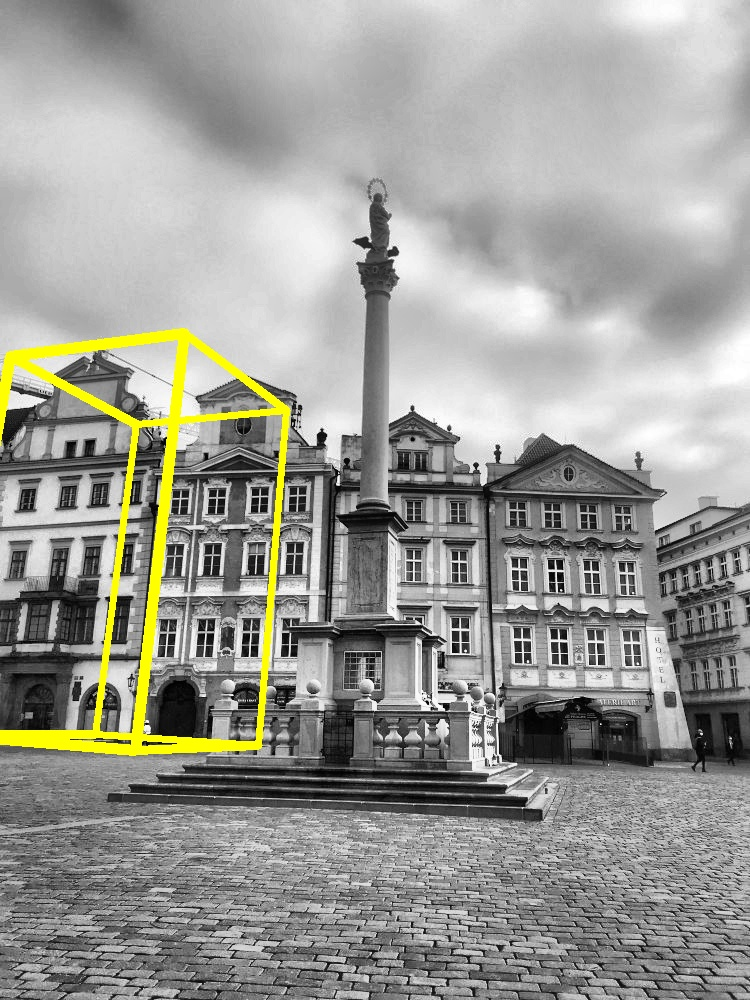
\includegraphics[width = 0.39\linewidth]{pictures/tests/1/sloup3_vol.jpg}
                    \caption[Detection of background building instead of foreground object]{Detection of a building in the background instead of the foreground object, after improving reference image of the detected building in the background. The test on the left image failed. Original photos: Tatiana Popova}
                    \label{fig:backgroundDetection}
                \end{figure}

    \FloatBarrier            
    \section{Installation}
        In this section, we provide a manual on how to install our project in a way that would be able to compile and run the prototype. We describe how to satisfy all the dependencies of the OpenCV and Boost C++ libraries. We have developed the prototype in the Visual Studio 2019 IDE on operating system Windows and the manual is written in a way to provide installation guide for this configuration.
        
        \subsection{Installing OpenCV}
            To run our prototype, it is needed to install OpenCV. There are two options for installing OpenCV. The first is to download the already built libraries and the second option is to compile the OpenCV codes. We write about two ways of installing, because there are some OpenCV modules that are not included in the official prebuilt binaries. Such a module is \textit{xfeatures2d} (extra/experimental 2D features algorithms), which is important for our project, because it contains the BEBLID algorithm.
            
            In both cases, the version 4.5.1 and higher has to be installed, because the BEBLID algorithm was introduced in this version. Also, the algorithm SIFT was already moved from the \textit{xfeatures2d} module to the regular \textit{features2d} module (2D features algorithms) in this OpenCV version.
            
            \subsubsection*{Installing prebuilt version}
                Installing the prebuilt version is more straightforward than compiling the library and installing it afterwards. The following manual is for installing OpenCV 4.5.2 for developing projects in Visual Studio 2019 on the operating system Windows. The steps of the installation are as follows:
                %
                \begin{enumerate}
                    \item Download the sources of the version 4.5.2 from the OpenCV releases page~\cite{OpenCVReleases},
                    \item Unpack the sources into desired location \texttt{<INSTALL\_ROOT>},
                    \item Run the \textit{Edit the system environment variables} tool and click the \textit{Environment Variables\dots} button,
                    \item When installing on the same account, create and edit the following variables in the table \textit{User Variables} otherwise in \textit{System Variables},
                    \item Create there a new \texttt{OPENCV452\_ROOT} variable with value \texttt{<INSTALL\_ROOT>\textbackslash},
                    \item Add \texttt{\%OPENCV452\_ROOT\%x64\textbackslash vc16\textbackslash bin} record for the \texttt{PATH} variable.
                \end{enumerate}
                %
                Follow next steps for installing OpenCV into Visual Studio project (the naming for \texttt{OPENCV452\_ROOT} may vary in different projects, so it is further called only \texttt{OPENCV\_ROOT}):
                %
                \begin{enumerate}
                    \item Create an empty C++ project in Visual Studio or download our project,
                    \item Open project properties,
                    \item Set the configuration (release/debug) that would be edited,
                    \item In the \textit{C/C++} section, open the \textit{General} subsection and add the \texttt{\$(OPENCV\_ROOT)include} record for \textit{Additional Include Directories} field,
                    \item If there are already some records in the fields, separate the records with semicolon,
                    \item In the \textit{Linker} section open the \textit{General} subsection and add \\ the~\texttt{\$(OPENCV\_ROOT)x64\textbackslash vc16\textbackslash lib\textbackslash} record in the \textit{Additional Library Directories} field,
                    \item In the \textit{Linker} section, open the \textit{Input} subsection and add \\ the~\texttt{opencv\_world452d.lib} record in the \textit{Additional Dependencies} field for debug configuration or \\\texttt{opencv\_world452.lib} for release configuration (configurations can be set at the top of the properties window),
                    \item It might be needed to restart the Visual Studio.
                \end{enumerate}
                %
                Further information may be found in the installation tutorial in the official OpenCV documentation~\cite{Gábor2021}.
            
            \subsubsection*{Compiling the library}
                For installing the library, it is best to follow the tutorial in the official OpenCV documentation~\cite{Gábor2021}. To compile OpenCV with the \textit{xfeatures2d} module, the CMAKE parameter \texttt{OPENCV\_EXTRA\_MODULES\_PATH} has to be set to \\ \texttt{opencv\_contrib/modules} where \texttt{opencv\_contrib} is a directory containing sources downloaded from the \textit{Repository for OpenCV's extra modules}. For our project it is also necessary to set the variable \texttt{BUILD\_opencv\_world} to true.
            \subsection{Installing Boost C++ Libraries}
                The second dependency of our project is the Boost C++ Libraries. We use the Boost version 1.76.0 in our project. To install Boost on Windows, the steps are following~\cite{BoostInstallWindows}:
                %
                \begin{enumerate}
                    \item Download and unpack the Boost ZIP file,
                    \item Go to the \texttt{tools\textbackslash build\textbackslash} directory,
                    \item Run bootstrap.bat,
                    \item Then run \texttt{b2 install --prefix=PREFIX} where the \texttt{PREFIX} is the directory to which is the Boost installed,
                    \item In a similar way as in the OpenCV installation manual, add a record \texttt{PREFIX\textbackslash bin} to the \texttt{PATH} system variable.
                \end{enumerate}
                %
                In our project, we have followed the installation manual from the official Boost documentation~\cite{BoostInstallWindows}. More information can be found there. So to run our project, following steps has to be taken during installing Boost to Visual Studio project:
                %
                \begin{enumerate}
                    \item Create a new system variable \texttt{BOOST176\_ROOT} with value \texttt{<PREFIX>\textbackslash}
                    \item Open the project properties,
                    \item Set the configuration (release/debug) that would be edited,
                    \item In the \textit{C/C++} section, open the \textit{General} subsection and add the\\ \texttt{\$(BOOST176\_ROOT)} record for the\textit{Additional Include Directories} field,
                    \item In the \textit{C/C++} section, open the \textit{Precompiled Headers} subsection, set \textit{Precompiled Header} field to \texttt{Not Using Precompiled Headers},
                    \item In the \textit{Linker} section, open the \textit{General} subsection and add the\\ \texttt{\$(BOOST176\_ROOT)stage\textbackslash lib} record in the \textit{Additional Library Directories} field,
                    \item If there are already some records in the fields, separate the records with a semicolon,
                    \item It might be needed to restart the Visual Studio.
                \end{enumerate}
                %


        \subsection{Running and compiling our prototype}
                To run and compile our prototype, it is necessary to install the OpenCV and Boost C++ libraries. The project was developed in Visual Studio 2019, so the easiest way to start is to also use the same IDE, because the manuals are created in that way.
                
                There are some further notes to the installation. When OpenCV without \textit{xfeatures2d} was installed, then the \texttt{COMPILE\_EXPERIMENTAL\_MODULES\_ENABLED} macro in the \textit{experimentalModules.h} header file has to be disabled. When compiling OpenCV manually, the \texttt{opencv\_world} has to be created, otherwise the additional library names in the project properties have to be specified differently. The system throws an error with the name of the missing library when running without them, so the names of the libraries can be found out by trying.
                
                When setting up the project and adding the additional library information in the project properties, the values may already be there if the project was downloaded by default.
                
    
    
\chapter{Future outlook}
    Despite the fact that it was not the task of our thesis, we considered creating a localisation module for the mobile application of the DTBQ project. We did not implement our own complete implementation, but we did a survey on how to create such a module and how to integrate it into already created code. We write about this in this chapter together with proposals for improving.
    
    \section{Contextualization}
        First, we want to put into the context of DTBQ what we have already created. We have tested and developed our prototype on images taken mainly in Prague, which is not a dowry town of bohemian queens, but we want to show that it can be easily used in the dowry towns as well. We also want to show how augmented reality could look based on our localisation.
        
        To do this, we have created a visualisation in figure~\ref{fig:prasnaKropacka}. In the image is a rendered model of the Kropáčka tower, which stood in the past in the dowry town Hradec Králové~\cite{Vojtiskova2019}. The render was stylised to match the night lighting conditions. But otherwise it was rendered based on the unchanged information given by our localisation prototype. The rendered tower does not cover the whole tower that was originally in the image (Prašná brána), because the sizes of both towers are different. But thanks to this, it is possible to see that the perspective of the rendered tower corresponds to that one of the original tower.
        
        \begin{figure}
            \centering
            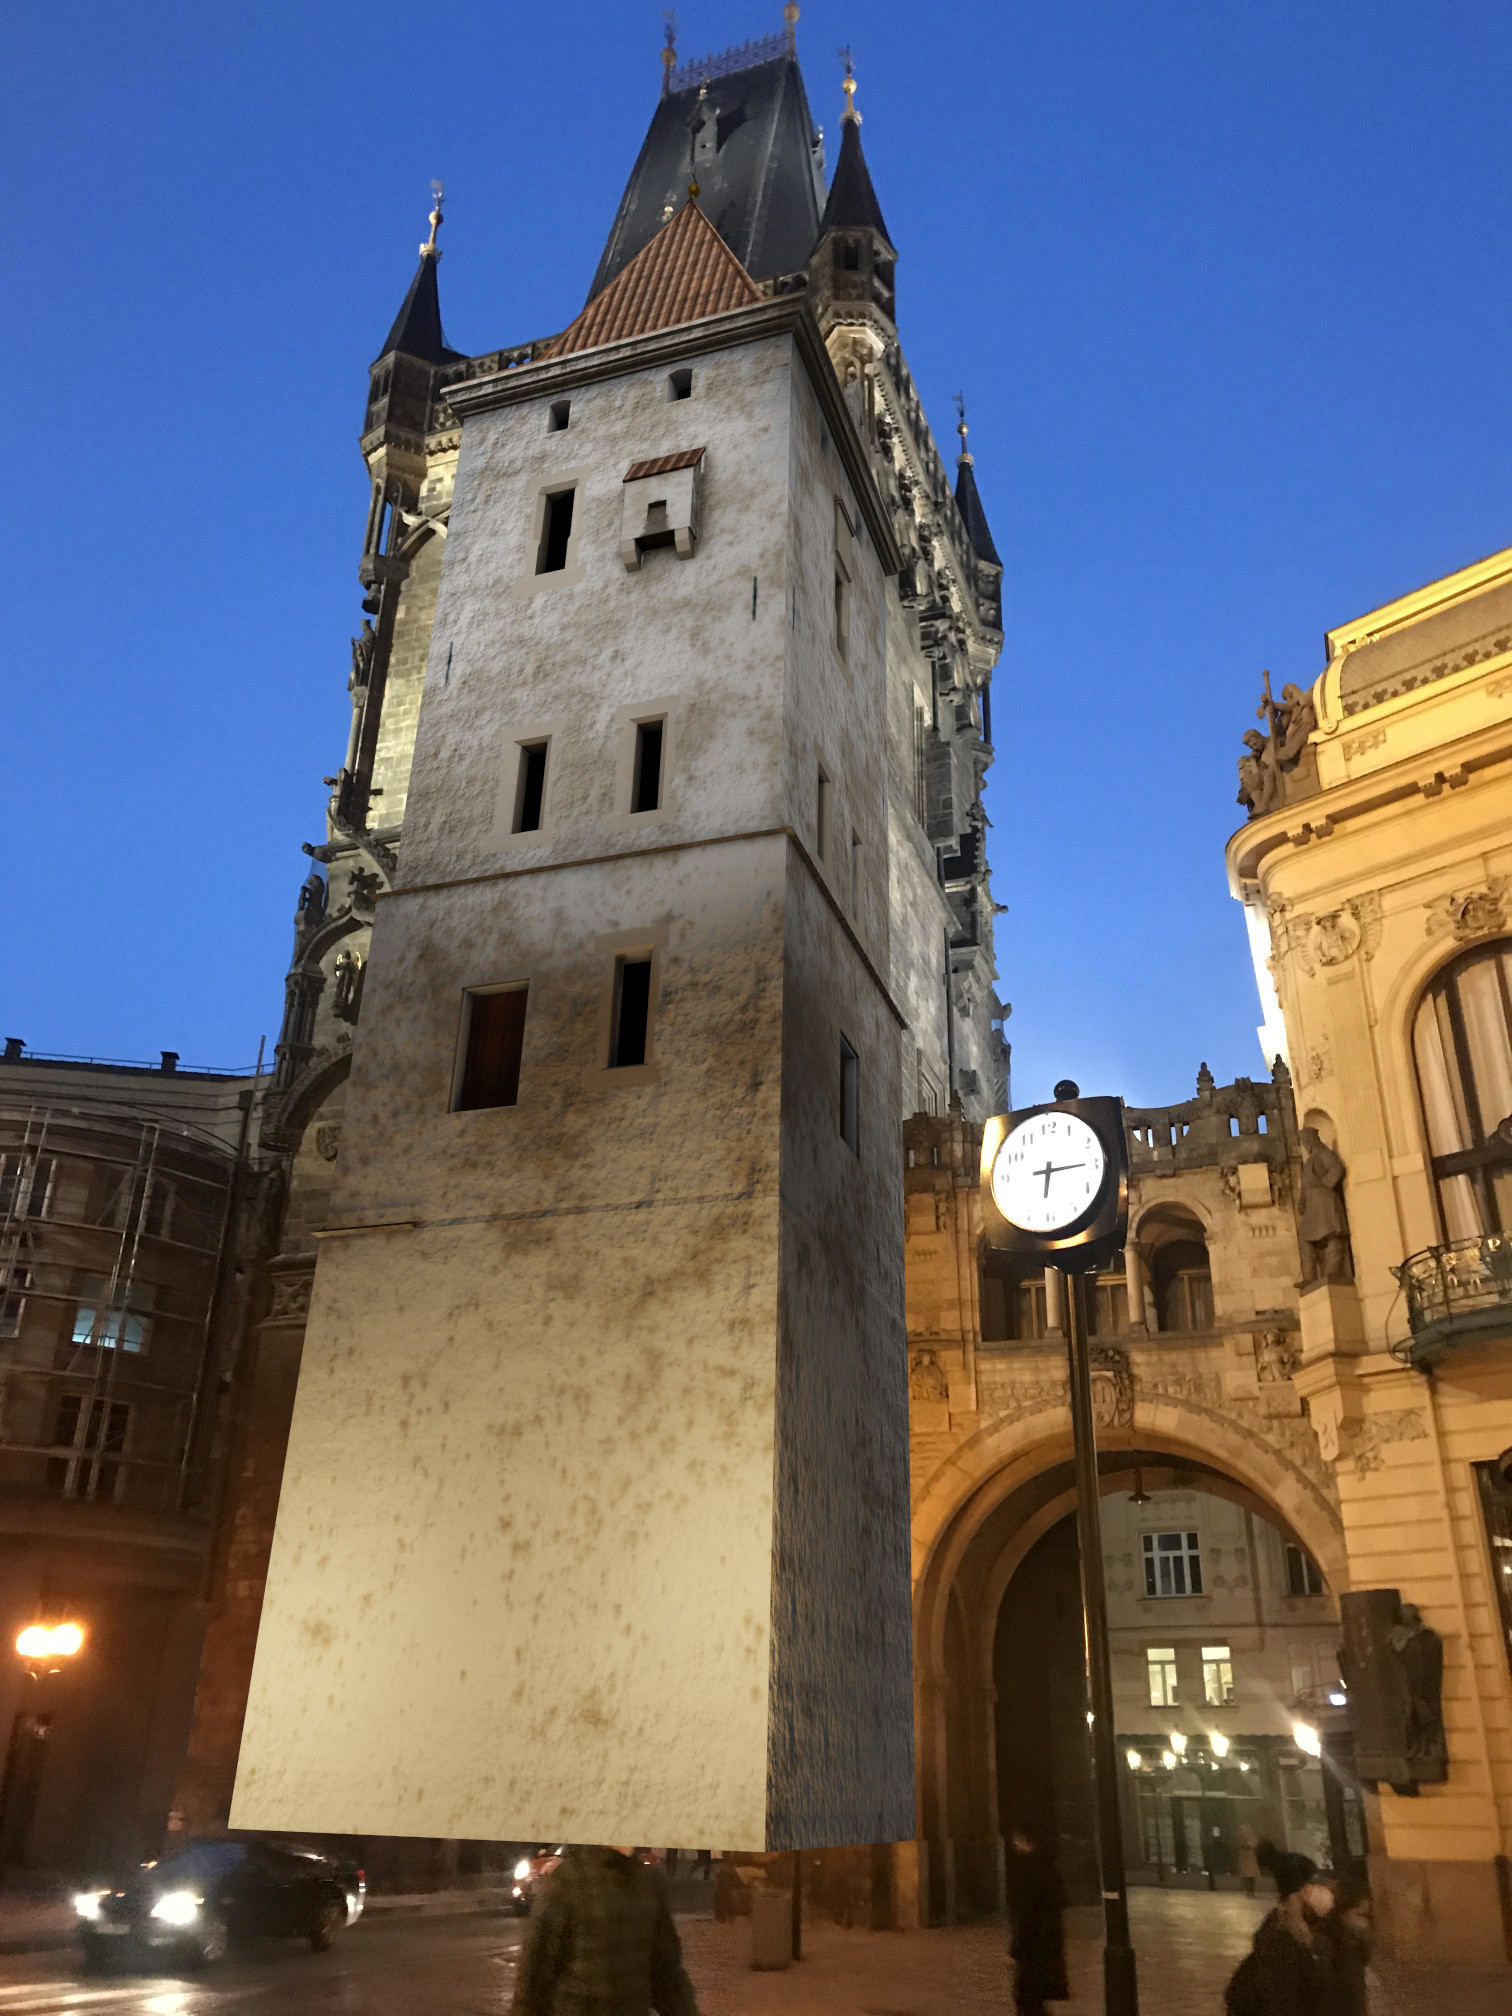
\includegraphics[width = 0.64\linewidth] {pictures/future/Kropatschka_Tower_instead_of_Prasna_Gate_small.jpg}
            \caption[Visualisation of the localisation with a 3D model of a tower Kropáčka]{Visualisation of the localisation with a 3D model of the Kropáčka tower. Environment photo was taken from the database of Tatiana Popova~\cite{Popova2021} and the 3D model was created as part of study~\cite{Vojtiskova2019}.}
            \label{fig:prasnaKropacka}
        \end{figure}
        
    \section{Design of the localisation module}
        We already specified and analysed the API and realisation of the localisation module by Jaroslav Štěpán in the section~\ref{sec:stepan}. We follow his design of the localisation module in most of the places. The part mediating the communication between the computing part and the application will be implemented in Java. The localisation module interface \texttt{ILocalizationModule} has to be implemented to create a localisation module in the application. The communication with the native code in C++ will be done via the Java Native Interface (JNI). The interface will have following methods:
        %
        \begin{itemize}
            \item \texttt{createProxyObject()},
            \item \texttt{destroyProxyObject()},
            \item \texttt{updateDatabase()},
            \item \texttt{getGlobalPosition()}.
        \end{itemize}
        %
        That list closely corresponds to the methods used in the JNI used in the local localisation prototype by Jaroslav Štěpán~\cite{Stepan2019}. The communication between the application, the Java part of the localisation module and the native code in C++ would look like in the sequence diagram~\ref{fig:sequenceDiagram}. The key point of the communication between the Java part of the module and the native code is to use a proxy object. The proxy object will be created on the heap memory and accessed using the address in the memory of the object whenever needed until it is released.
        %
        \begin{figure}
            \centering
            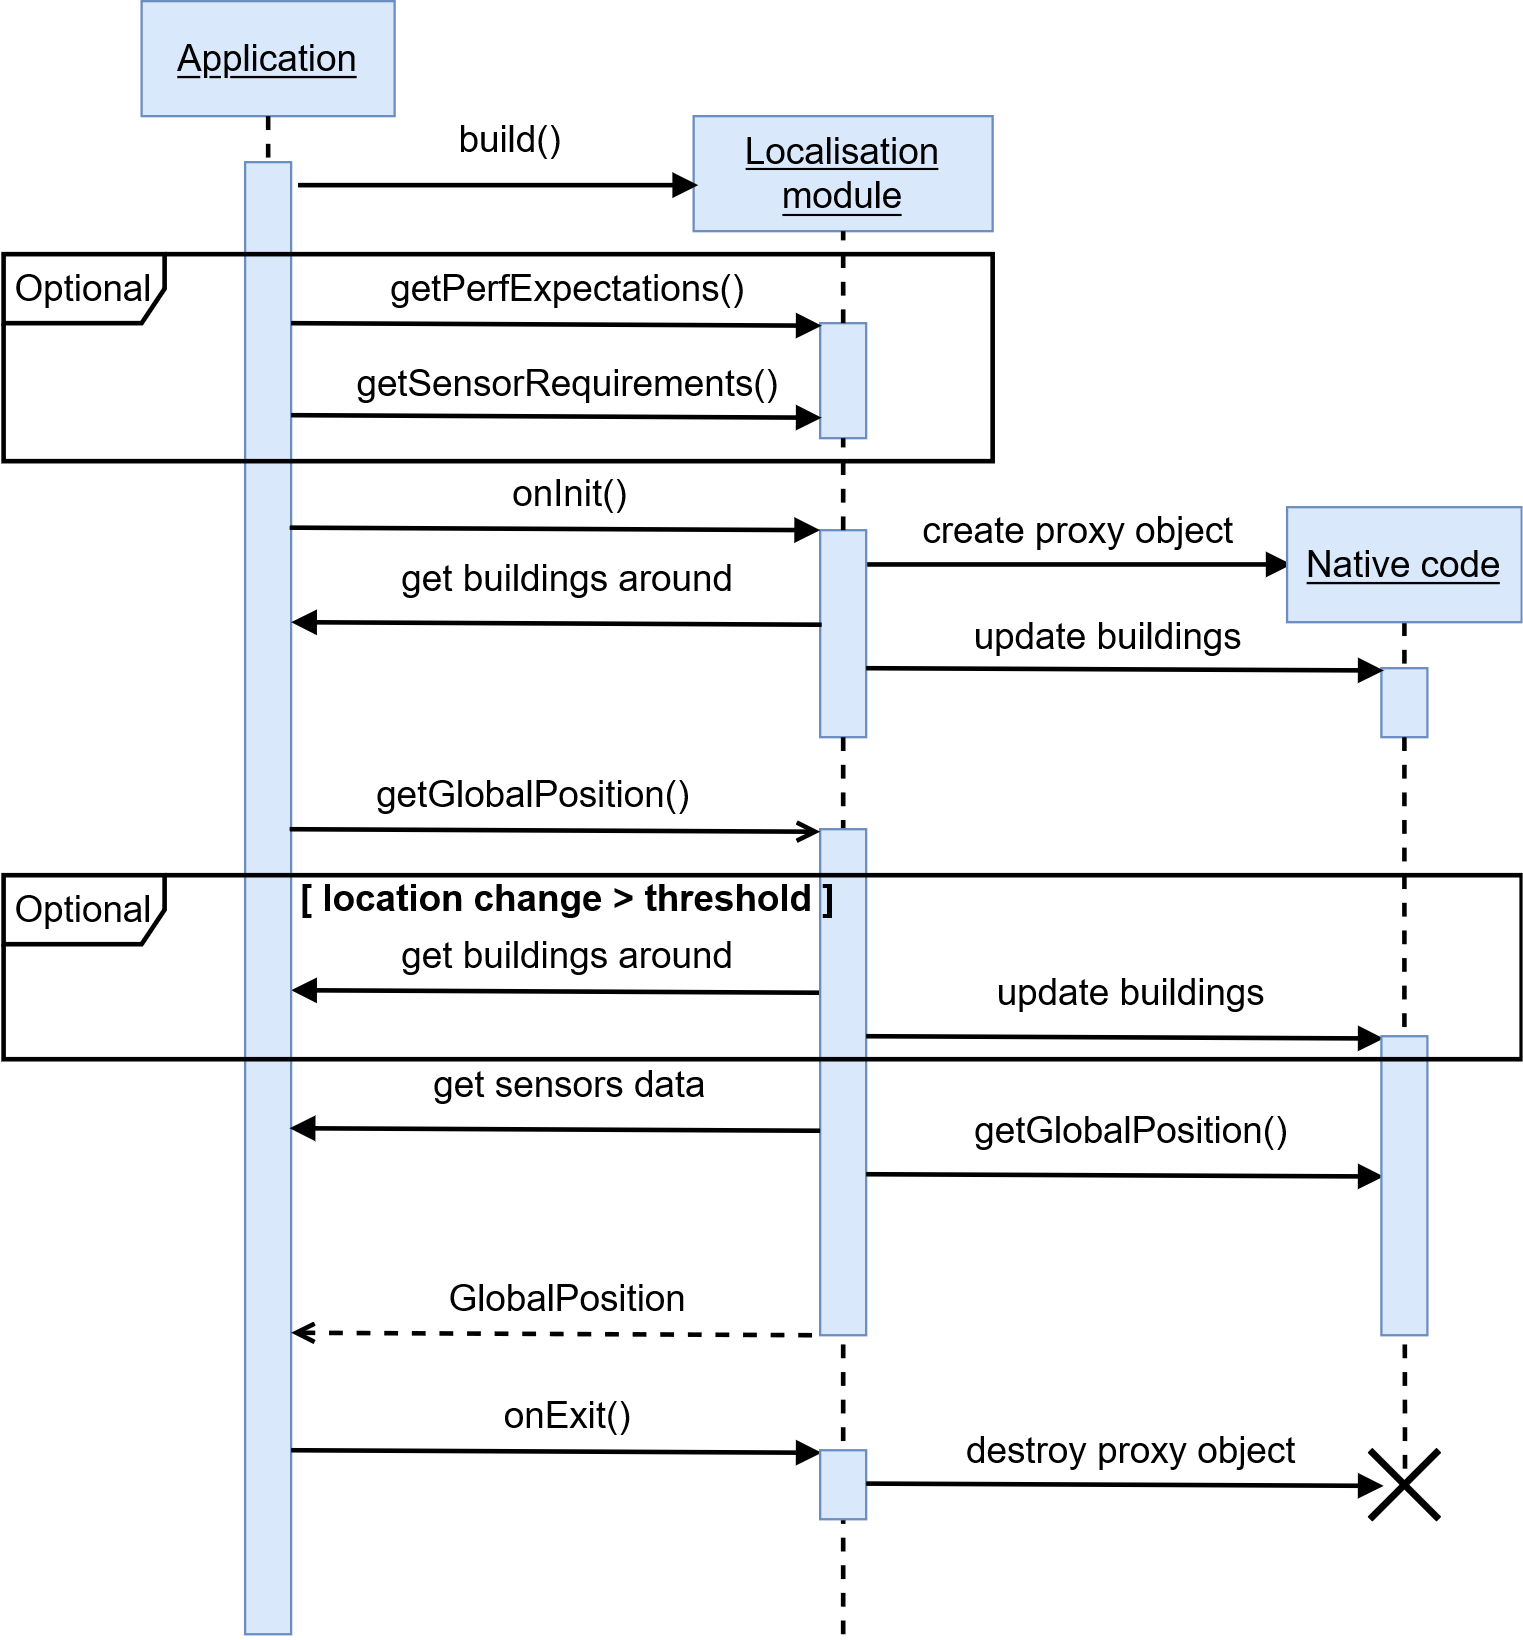
\includegraphics[width = 1\linewidth]{pictures/future/sequenceDiagram2.png}
            \caption{Sequence diagram of the communication between the application, localisation module and native code}
            \label{fig:sequenceDiagram}
        \end{figure}
        %
        The following list is an explanation of some called functions in the sequence diagram~\ref{fig:sequenceDiagram}:
        \begin{description}
            \item[\texttt{getPerfExpectations()}] Method implemented by the localisation module that returns information about what hardware usage the module would have.
            \item[\texttt{getSensorRequirements()}] Method returning what sensors the module needs to operate with.
            \item[\texttt{getGlobalPosition()}] Method that is called by the application to get the location.
        \end{description}
        
        \subsection{Integration of the already finished code}
            A big part of the already created code could be moved into the module. The main part that would have to be redone is the input loading and processing configuration. The prototype is not planned to store the images for a longer time for multiple processing. Therefore, it would be appropriate to create a run-time database of reference images inside the native code. The database would be updated whenever the device location would be changed more than by pre-defined the threshold. In the run-time database would be prepared descriptors of reference buildings images for next calculation of the global location, so that the response would be as fast as possible. The rest of the code would be also optimised to get even better performance, mainly because some parts of the prototype are redundant for the module inside the mobile application. But the main processing part of the prototype could be just modified in a way that it would be possible to run it directly after calling the \texttt{getGlobalPosition} method of the proxy object.
    
    \section{Future improvements proposals}
        Here we want to present some improvement proposals of the processing that we are aware of but we did not have the time frame to realise them.

            \subsubsection*{Precise reference images}
            We have observed in the tests that the quality of reference images is a crucial factor, especially the image aspect ratio has to be on point. Unfortunately we do not have that much precise reference images of buildings yet, because we do not know the exact size of the buildings facades. The loss of accuracy by not having precise reference images is well illustrated in the image~\ref{possibleGainOfAccuracy}. By having more precise references images not only the loss will diminish but also the detection would be more successful as well. So we see that as the most important point of improvement.
            
            \begin{figure}
                \centering
                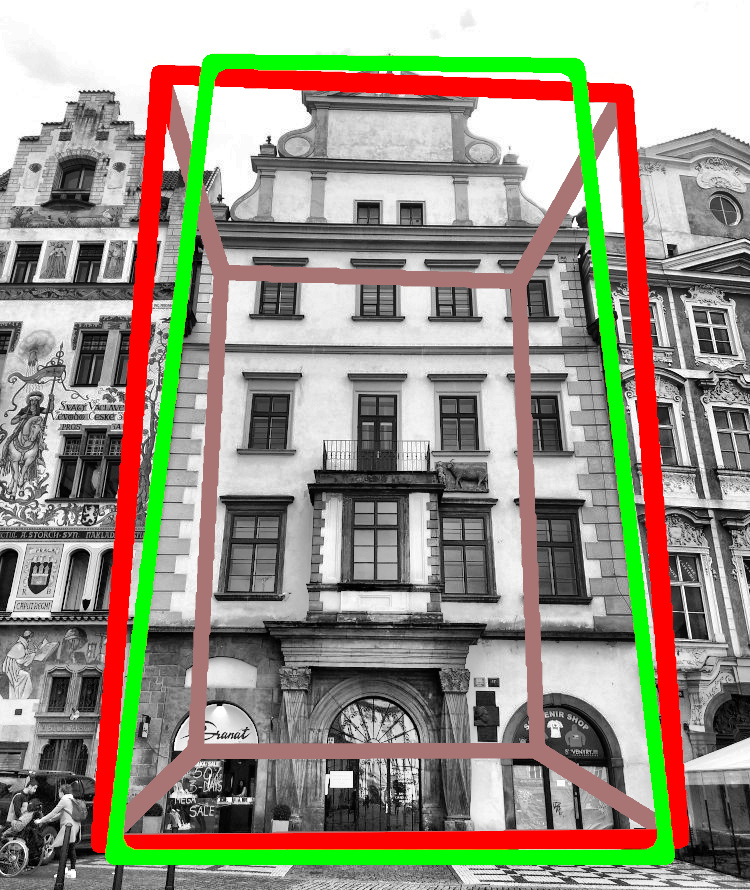
\includegraphics[width = 0.5\linewidth]{pictures/future/possibleAccuracyGain.jpg}
                \caption[Possible gain of accuracy in case of improving reference images]{Possible gain of accuracy in case of improving reference images. The green quadrilateral is what has been detected and the red quadrilateral is the final product of a volume understanding. The difference between them is then the accuracy loss that was caused by having inaccurate reference images. Photo: author}
                \label{possibleGainOfAccuracy}
            \end{figure}

            \subsubsection*{ASIFT}
            We discovered the ASIFT algorithm in the OpenCV documentation just as we were finishing our thesis, so we did not have enough time to research this method anymore. It is implemented in OpenCV under the name \texttt{AffineFeature} as a part of the \textit{features2d} module. The ASIFT algorithm is a modification of the SIFT algorithm that improves the SIFT affine transformations invariance~\cite{yu2011asift}. This could help to detect buildings, even if they were photographed from a sharper angle.
        
        \subsection{Future modules data requirements}
            In this section we write about the possible future improvement of the localisation that would require more input data than what we specified in the section~\ref{sec:InputOutputFormats}.
            
            \subsubsection*{Localisation in hilly areas}
                The localisation in hilly areas is problematic if we want to know the global coordinates of the mobile device, because the altitude is not included in the format of the global coordinates. In this case, it would be necessary to know the precise real world up~vector, which could be obtained from the phone sensors or calculated if the detected object has a vertical facade. Another requirement would be to have access to the altitude for the given coordinates. With this information, it would be possible to calculate the exact location even in hilly areas, for example by an iterative method with an initial estimate of the altitude from the phone sensors.
                
            \subsubsection*{Buildings given based on location}
                Another improvement would be if the API of the mobile application gave the module only objects that are inside a circle with a given radius and center around some global coordinates.
                
            \subsubsection*{Descriptors instead of images}
                To detect objects, it is only needed to have the descriptors of the features detected in the reference image. So it would be better to use already precalculated descriptors of the reference images in the application. It would be appropriate if the descriptors were precalculated by multiple methods. Because then it would be possible to use faster (but less accurate) feature detection and extraction methods for devices with lower computation power and vice versa.
                
            \subsubsection*{Dynamical scaling of scene images}
            Despite the fact that the used local image features are to some extent invariant to the scale of the image they have been detected in, the feature is more likely to be detected in both of two different images if their scale is similar. The scene image would be probably scaled anyway to improve the speed of the computations. For this reason it would be convenient to scale the image so the building in the scene image has a similar resolution as the resolution of the image in the database. This can be achieved by guessing the scale factor from the distance between the location of the phone and the building based on the output of the phone positioning sensors.
                
\begin{conclusion}
    We continued the work started by Jan Šefčík. We improved the image recognition processing and moved the localisation from within image object localisation into 3D space and real world localisation. First, we have researched the used technologies, the \textit{Dowry Towns of Bohemian Queens} project and the theses within the project connected to our. After that we analysed the researched technologies, theses and technologies used in the project. There we described the concepts of current designs and realisations already created in the project and then explained the changes we want to make in the design. Based on this, we realised a prototype of mobile device localisation based on image recognition. We wanted to show the performance of the prototype on tests created with the intention of getting as close as possible to the future use of the localisation module. These tests have shown that the device localisation based on image recognition is, on average, more accurate than phone sensors. Also we have observed that by having better quality of reference images the accuracy and reliability will get even higher by recognisable margin.
    
During the solution, we considered making not only the prototype but also the localisation module for the DTBQ application. Unfortunately this was not possible because the application itself was prepared only one month before the thesis submission deadline. We wanted to finish a fully functional localisation solution, so we spent the rest of the time completing the prototype.
    
    In addition, we outlined the future development of the localisation application module.
We have gained a lot of knowledge about this issue and we would like to help develop the \textit{Dowry Towns of Bohemian Queens} project by finishing the localisation module for the mobile application. Therefore, we plan to continue working on it also after submitting the bachelor thesis.
\end{conclusion}
 
    

\printbibliography[title={Bibliography}]

%\bibliographystyle{csn690}
%\bibliography{mybibliographyfile}

\appendix

\chapter{List of used abbreviations}
% \printglossaries
\begin{description}
    \item[AHE] Adaptive histogram equalisation
    \item[API] Application programming interface
    \item[BEBLID] Boosted efficient binary local image descriptor
    \item[BELID] Boosted efficient local image descriptor
    \item[CIE] International Commission on Illumination
    \item[CLAHE] Contrast limited adaptive histogram equalization
    \item[CRUD] Create, read, update, and delete
    \item[DTBQ] Dowry Towns of Bohemian Queens
    \item[FLANN] Fast Library for Approximate Nearest Neighbors
    \item[GPS] Global Positioning System
    \item[IDE] Integrated development environment
    \item[JNI] Java native interface
    \item[LBP] Local binary patterns
    \item[ORB] Oriented FAST and Rotated BRIEF
    \item[PnP problem] Perspective-n-Point problem
    \item[RANSAC] Random Sample Consensus
    \item[SIFT] Scale-invariant feature transform

\end{description}

\chapter{Contents of the attached data storage}

%upravte podle skutečnosti

\begin{figure}
    \dirtree{%
        .1 readme.txt\DTcomment{brief description of the data storage contents }.
        .1 exe\DTcomment{directory with executable form of implementation}.
        .2 image\_database\DTcomment{image database}.
        .2 config\DTcomment{directory with configuration}.
        .1 src.
        .2 impl\DTcomment{implementation source codes}.
        .2 thesis\DTcomment{source form of work in \LaTeX{} format}.
        .1 text\DTcomment{thesis text}.
        .2 thesis.pdf\DTcomment{thesis text in PDF format}.
    }
\end{figure}

\chapter{Test results}

In this appendix are all the results from testing. They are in the form of two pictures and a caption. The left picture is an aerial map, where the detected building's facade is marked with a yellow line. The global location calculated by our prototype is then located at the tip of the green pin and the location detected by the phone sensor is at the tip of the cyan pin. The right image represents the recognised volume of the building (the place where the building is located). It should be taken into account that the aerial map may not accurately correspond to the real location of the buildings. All the input scene photos were taken by us or from the image database by Tatiana Popova~\cite{Popova2021}.


The caption has the following format: \textbf{Our:} global coordinates; \textbf{phone:} global coordinates; \textbf{difference:} distance; \textbf{note:}(optionally) text. Where \textbf{Our} represents a field with the global coordinates calculated by our prototype and \textbf{phone} then those which have been detected by the phone positioning sensor. \textbf{Difference} is then the distance between \textbf{Our} and \textbf{phone}. The distance value is preceded by a plus if the result was evaluated as more accurate for \textbf{Our} or a minus if the \textbf{phone} was more accurate. The question mark is then used for undecidable cases and -\(\infty\) where our prototype failed (then there is also no green pin on the map).


\begin{figure}
    \centering
    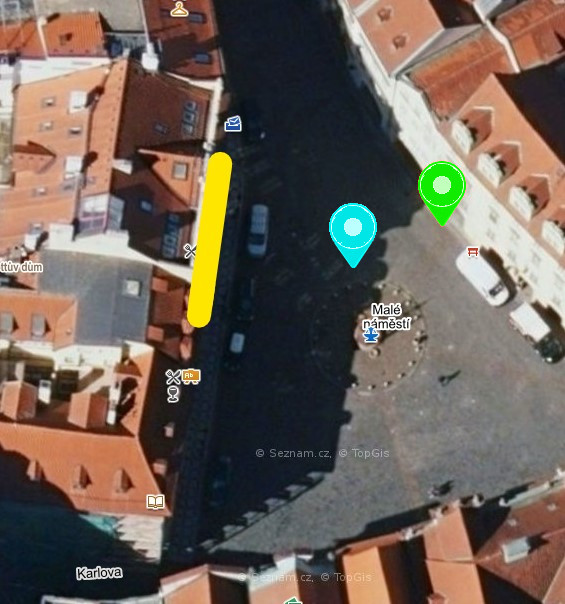
\includegraphics[width = 0.35\linewidth]{pictures/tests/1/dum_Rott_loc.jpg}
    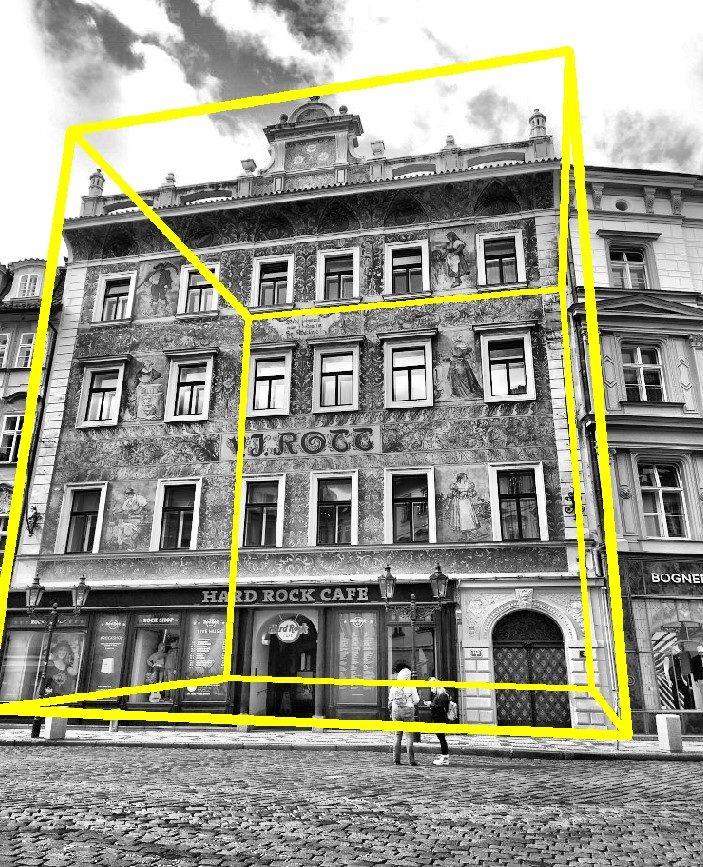
\includegraphics[width = 0.30\linewidth]{pictures/tests/1/dum_Rott_vol.jpg}
    \caption[Test result 1]{Our: 50.0867079, 14.4196045; phone: 50.0866778, 14.4194886; difference: +8.92 m. Source of the aerial map: Mapy.cz}
    \label{fig:test1-round1}
\end{figure}

\begin{figure}
    \centering
    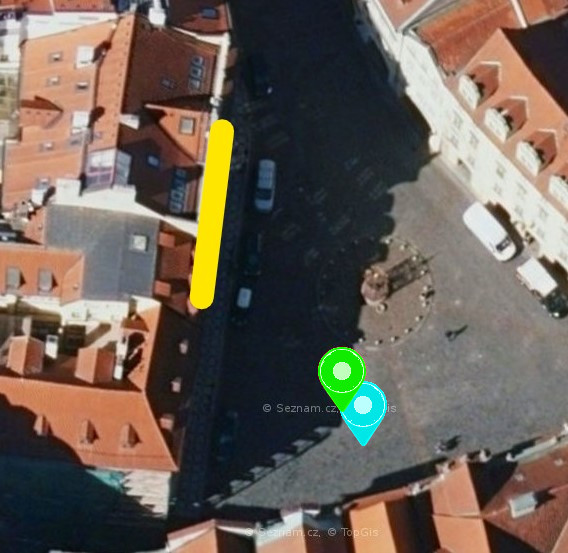
\includegraphics[width = 0.35\linewidth]{pictures/tests/1/dum_Rott2_loc.jpg}
    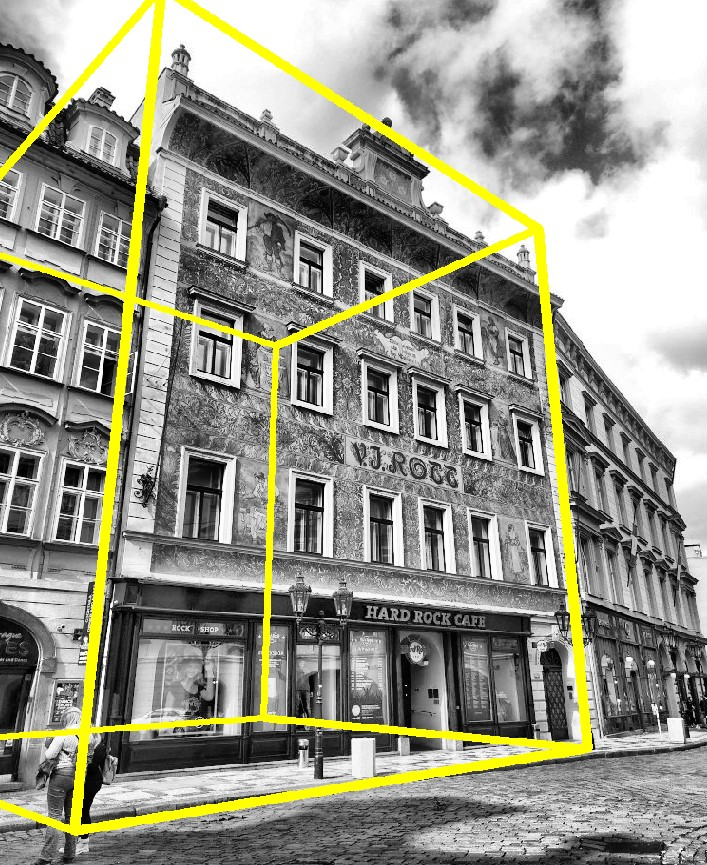
\includegraphics[width = 0.30\linewidth]{pictures/tests/1/dum_Rott2_vol.jpg}
    \caption[Test result 2]{Our: 50.0865094, 14.4194608; phone: 50.0864750, 14.4194681; difference: ?3.86 m. Source of the aerial map: Mapy.cz}
    \label{fig:test1-round2}
\end{figure}

\begin{figure}
    \centering
    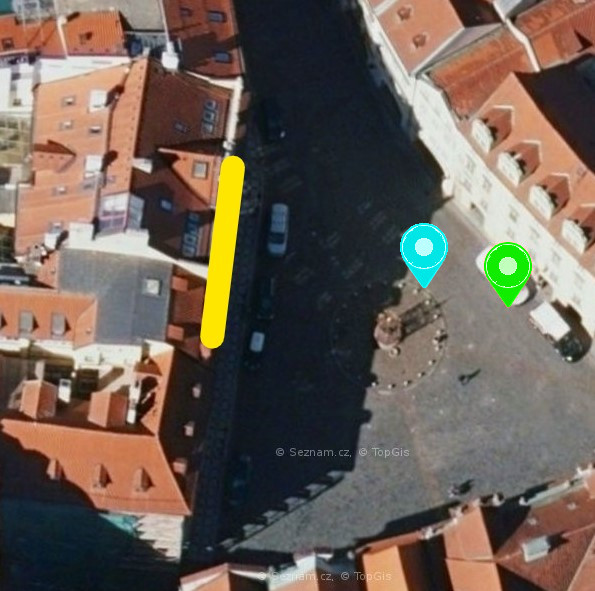
\includegraphics[width = 0.35\linewidth]{pictures/tests/1/dum_Rott3_loc.jpg}
    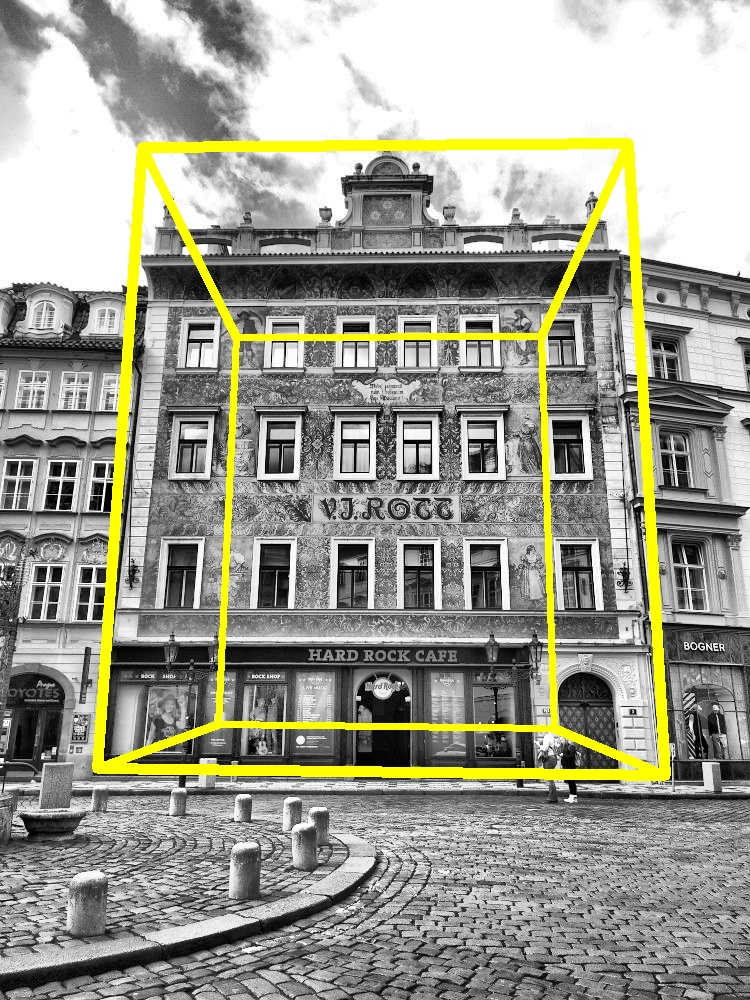
\includegraphics[width = 0.30\linewidth]{pictures/tests/1/dum_Rott3_vol.jpg}
    \caption[Test result 3]{Our: 50.086637, 14.4196669; phone: 50.0866556, 14.4195519; difference: +8.46 m. Source of the aerial map: Mapy.cz}
    \label{fig:test1-round3}
\end{figure}

\begin{figure}
    \centering
    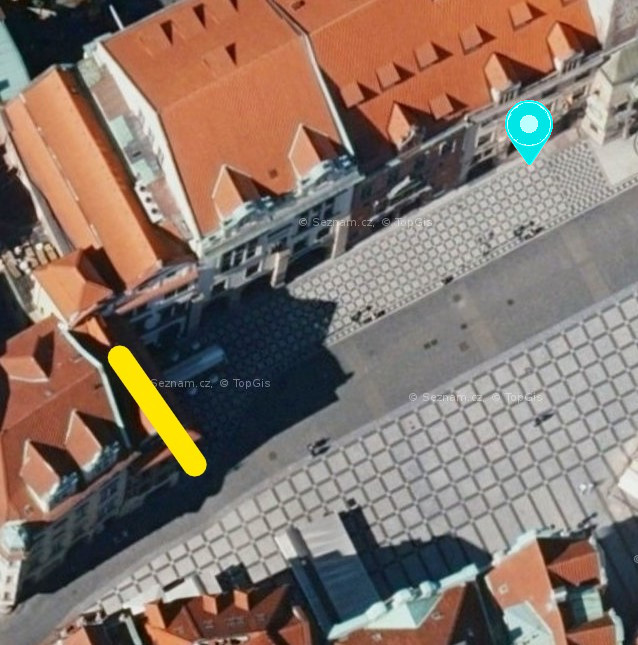
\includegraphics[width = 0.35\linewidth]{pictures/tests/1/Dum_u_minuty_loc.jpg}
    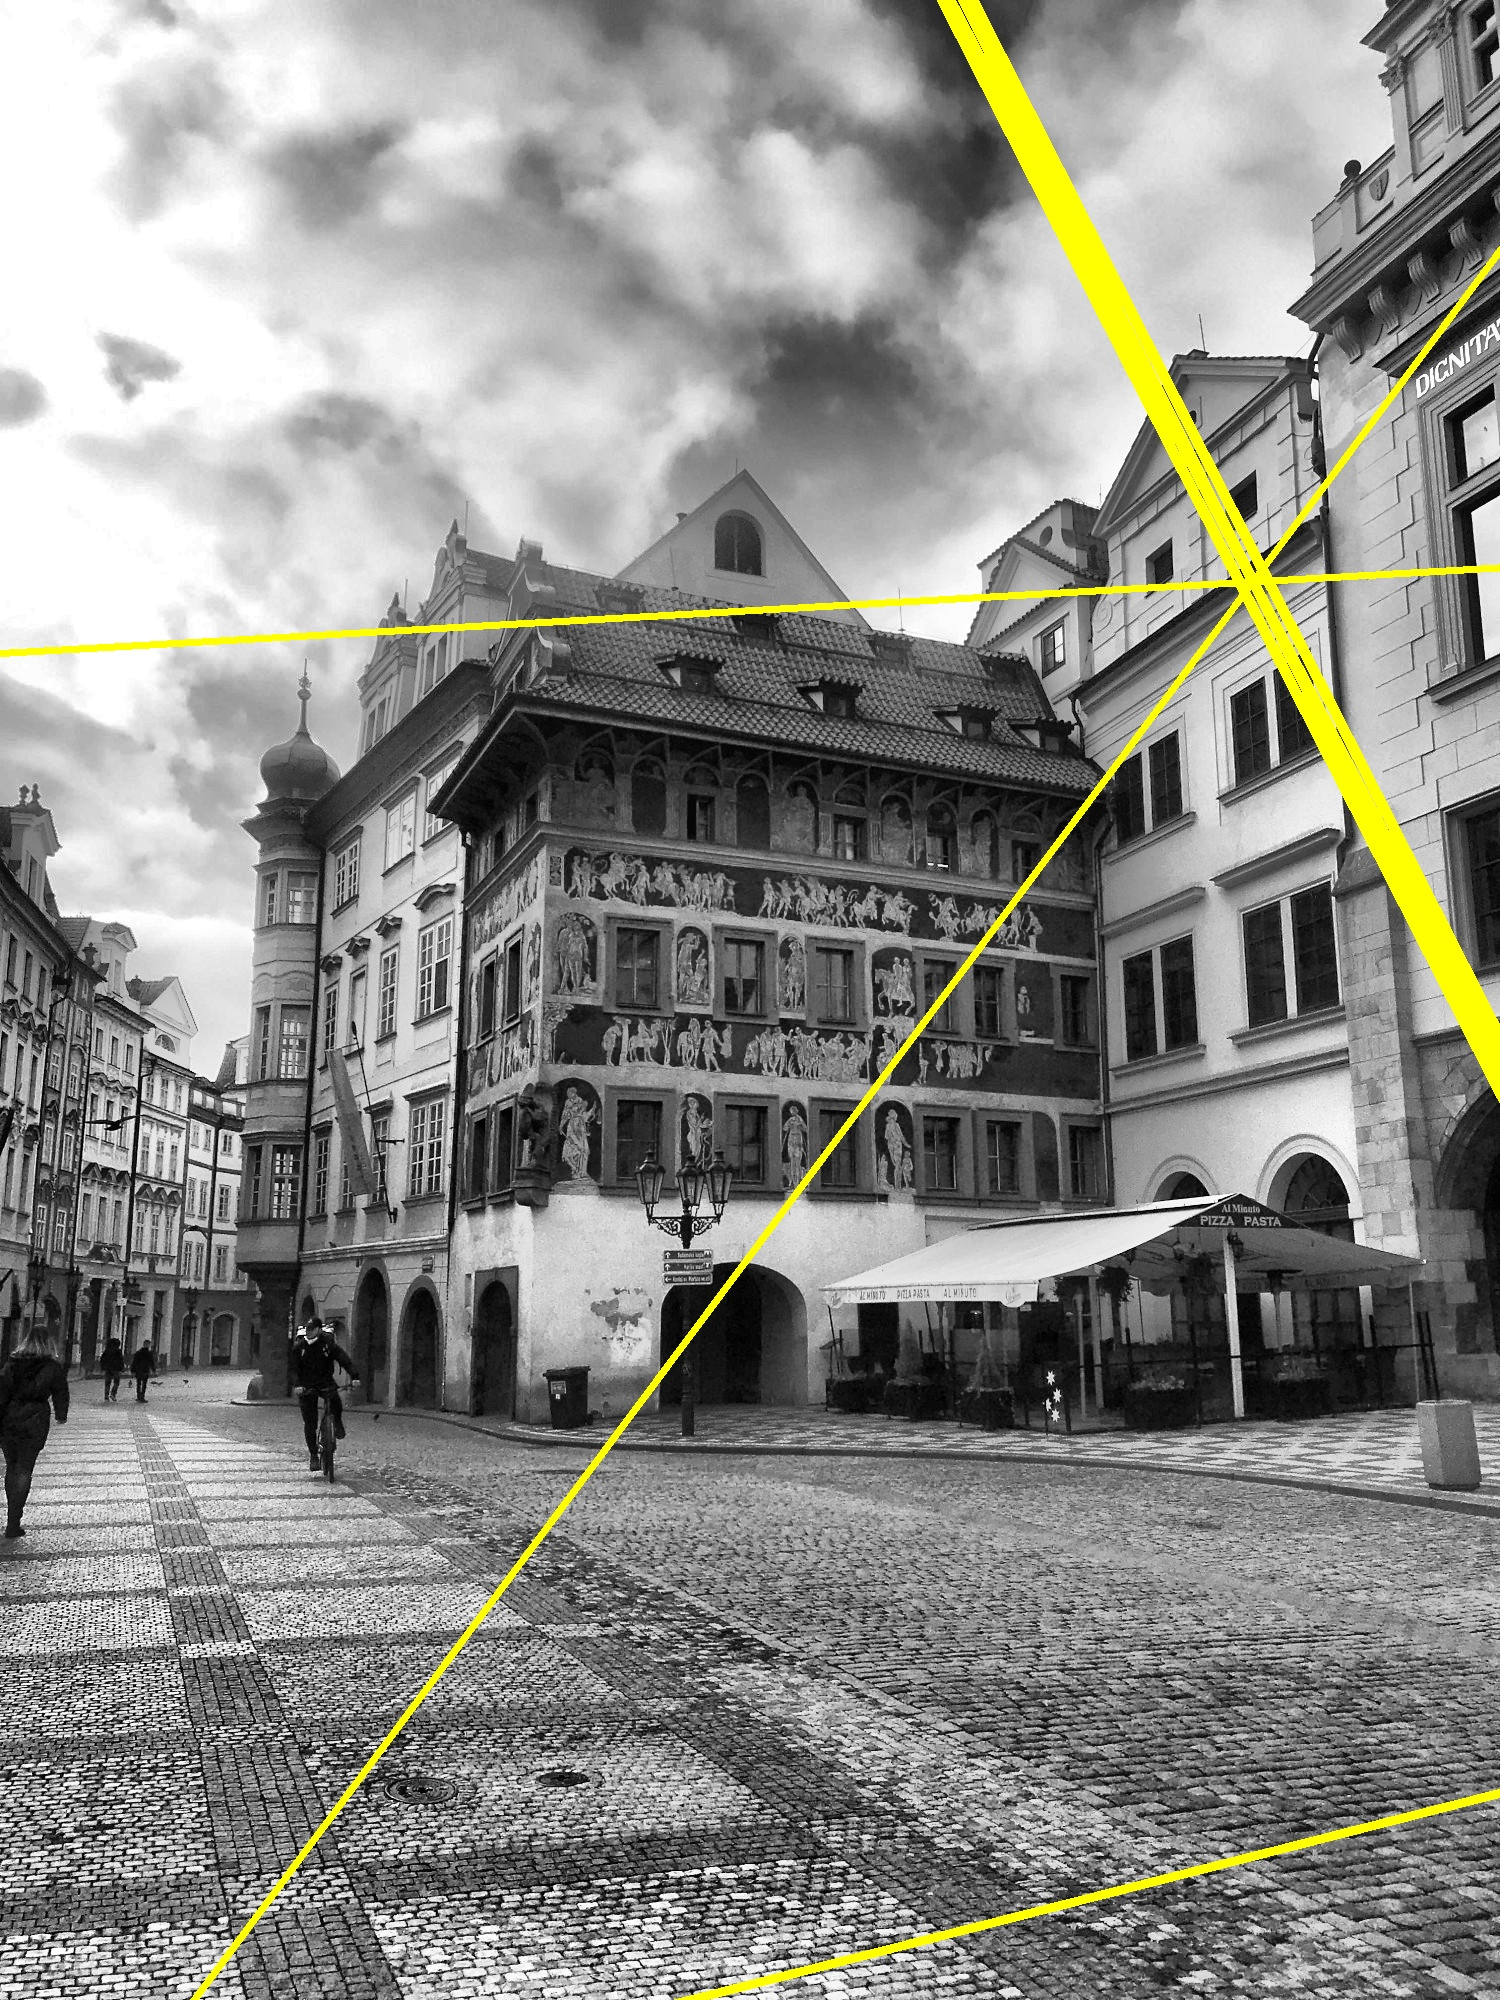
\includegraphics[width = 0.30\linewidth]{pictures/tests/1/Dum_u_minuty_vol.jpg}
    \caption[Test result 4]{Our: 50.0872907, 14.4213531; phone: 50.0869444, 14.4205556; difference: -\(\infty\) m. Source of the aerial map: Mapy.cz}
    \label{fig:test1-round4}
\end{figure}

\begin{figure}
    \centering
    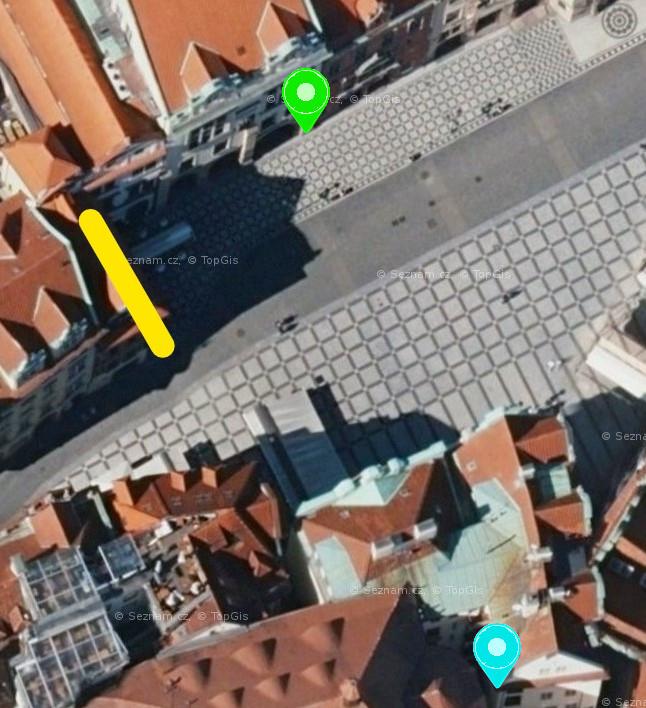
\includegraphics[width = 0.35\linewidth]{pictures/tests/1/Dum_u_minuty2_loc.jpg}
    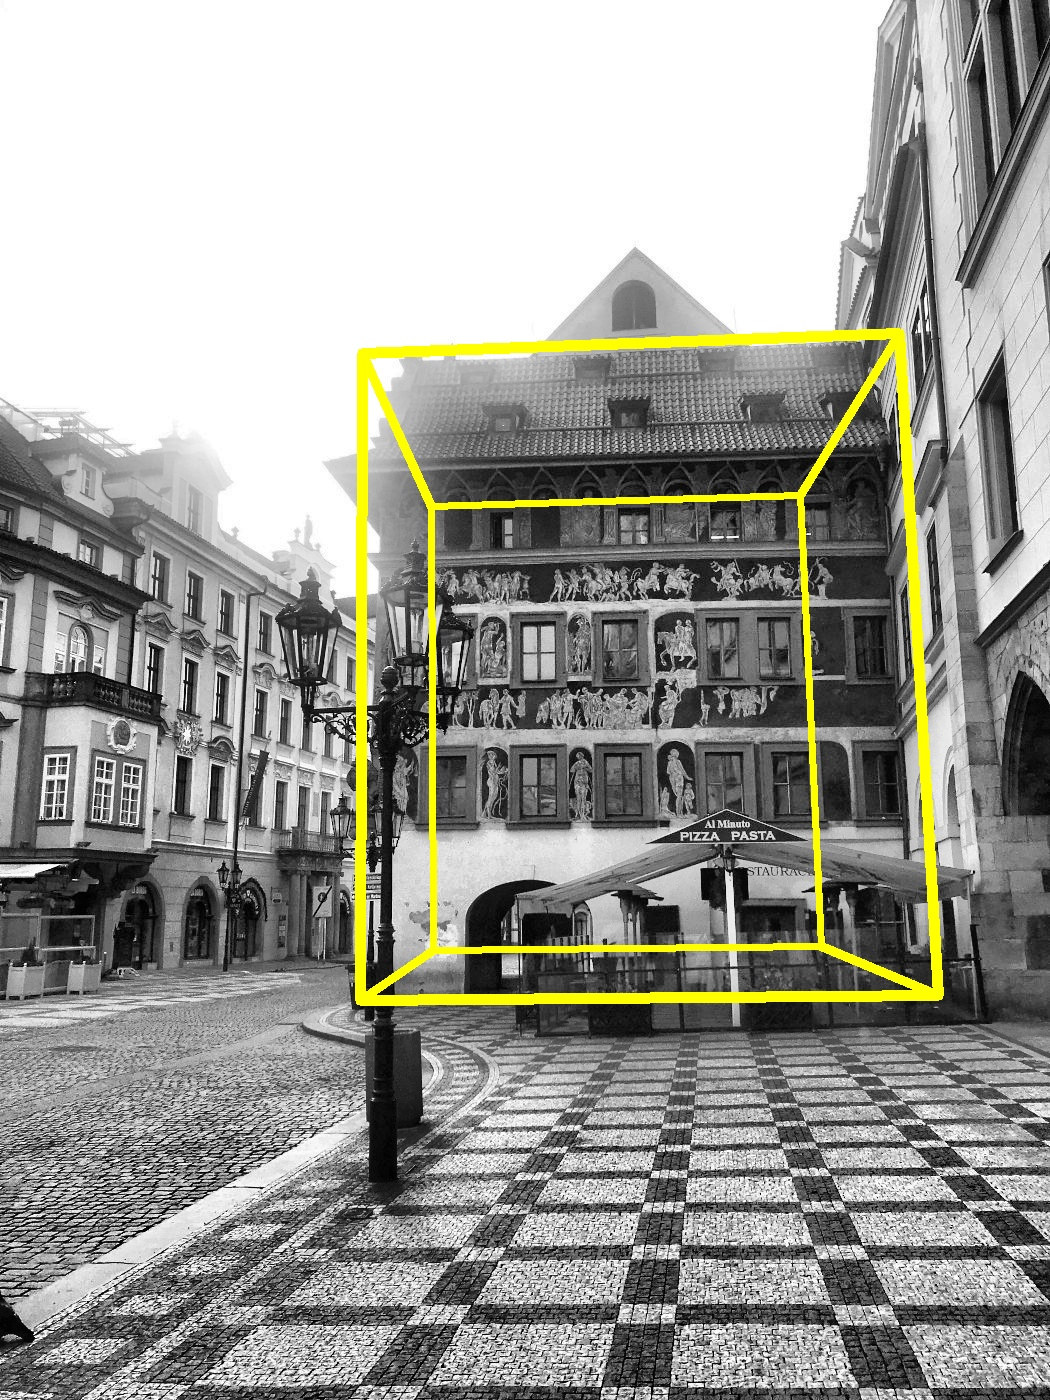
\includegraphics[width = 0.30\linewidth]{pictures/tests/1/Dum_u_minuty2_vol.jpg}
    \caption[Test result 5]{Our: 50.0868708, 14.420301; phone: 50.0863889, 14.4205556; difference: +56.58 m. Source of the aerial map: Mapy.cz}
    \label{fig:test1-round5}
\end{figure}

\begin{figure}
    \centering
    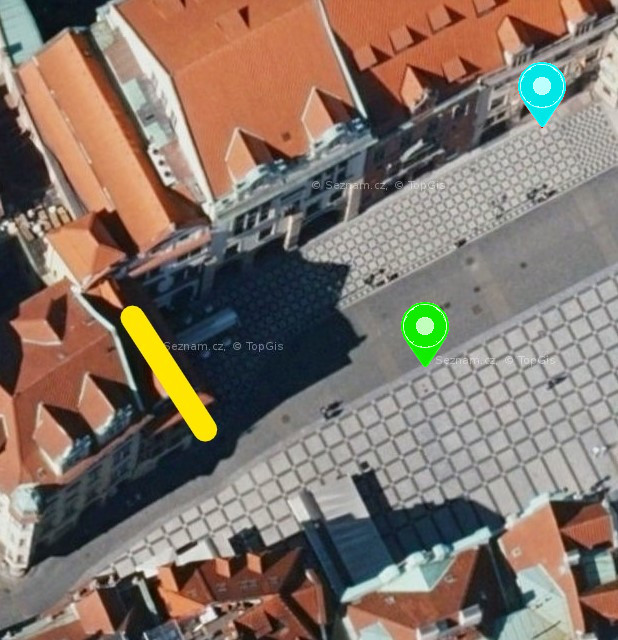
\includegraphics[width = 0.35\linewidth]{pictures/tests/1/Dum_u_minuty3_loc.jpg}
    \includegraphics[width = 0.30\linewidth]{pictures/tests/1/Dum_u_minuty3_vol.jpg}
    \caption[Test result 6]{Our: 50.0867419, 14.4204009; phone: 50.0869444, 14.4205556; difference: +25.08 m. Source of the aerial map: Mapy.cz}
    \label{fig:test1-round6}
\end{figure}

\begin{figure}
    \centering
    \includegraphics[width = 0.35\linewidth]{pictures/tests/1/Jecna_loc.jpg}
    \includegraphics[width = 0.30\linewidth]{pictures/tests/1/Jecna_vol.jpg}
    \caption[Test result 7]{Our: 50.0755673, 14.4229881; phone: 50.0758333, 14.4230556; difference: +29.97 m. Source of the aerial map: Mapy.cz}
    \label{fig:test1-round7}
\end{figure}

\begin{figure}
    \centering
    \includegraphics[width = 0.35\linewidth]{pictures/tests/1/Jecna2_loc.jpg}
    \includegraphics[width = 0.30\linewidth]{pictures/tests/1/Jecna2_vol.jpg}
    \caption[Test result 8]{Our: 50.0755462, 14.4227431; phone: 50.0758333, 14.4227778; difference: +32.02 m. Source of the aerial map: Mapy.cz}
    \label{fig:test1-round8}
\end{figure}

\begin{figure}
    \centering
    \includegraphics[width = 0.35\linewidth]{pictures/tests/1/Prasna_brana_loc.jpg}
    \includegraphics[width = 0.30\linewidth]{pictures/tests/1/Prasna_brana_vol.jpg}
    \caption[Test result 9]{Our: 50.0870019, 14.4284049; phone: 50.0871414, 14.4285222; difference: ?17.63 m. Source of the aerial map: Mapy.cz}
    \label{fig:test1-round9}
\end{figure}

\begin{figure}
    \centering
    \includegraphics[width = 0.35\linewidth]{pictures/tests/1/Prasna_brana2_loc.jpg}
    \includegraphics[width = 0.30\linewidth]{pictures/tests/1/Prasna_brana2_vol.jpg}
    \caption[Test result 10]{Our: 50.0857078, 14.4191975; phone: 50.0872222, 14.4280556; difference: -\(\infty\) m. Source of the aerial map: Mapy.cz}
    \label{fig:test1-round10}
\end{figure}

\begin{figure}
    \centering
    \includegraphics[width = 0.35\linewidth]{pictures/tests/1/Prasna_brana3_loc.jpg}
    \includegraphics[width = 0.30\linewidth]{pictures/tests/1/Prasna_brana3_vol .jpg}
    \caption[Test result 11]{Our: 50.0872281, 14.4282983; phone: 50.0872222, 14.4280556; difference: +17.33 m; note: In comparison to the test~\ref{fig:test1-round10} this test was done after the night reference building image was added to the database. Source of the aerial map: Mapy.cz}
    \label{fig:test1-round11}
\end{figure}

\begin{figure}
    \centering
    \includegraphics[width = 0.35\linewidth]{pictures/tests/1/Prasna_brana4_loc.jpg}
    \includegraphics[width = 0.30\linewidth]{pictures/tests/1/Prasna_brana4_vol.jpg}
    \caption[Test result 12]{Our: 50.0870014, 14.4284044; phone: 50.0871414, 14.4285222; difference: ?17.69 m; note: In comparison to test~\ref{fig:test1-round9} this test was done after the night reference building image was added to the database. Small difference in output was created, because the Lowe's ratio threshold was changed from 0.7 to 0.75. Source of the aerial map: Mapy.cz}
    \label{fig:test1-round12}
\end{figure}

\begin{figure}
    \centering
    \includegraphics[width = 0.35\linewidth]{pictures/tests/1/sloup_loc.jpg}
    \includegraphics[width = 0.30\linewidth]{pictures/tests/1/sloup_vol.jpg}
    \caption[Test result 13]{Our: 50.087235, 14.4213759; phone: 50.0872222, 14.4213889; difference: ?1.70 m. Source of the aerial map: Mapy.cz}
    \label{fig:test1-round13}
\end{figure}

\begin{figure}
    \centering
    \includegraphics[width = 0.35\linewidth]{pictures/tests/1/sloup2_loc.jpg}
    \includegraphics[width = 0.30\linewidth]{pictures/tests/1/sloup2_vol.jpg}
    \caption[Test result 14]{Our: 50.0669414, 14.4487256; phone: 50.0875000, 14.4213889; difference: -\(\infty\) m; note: The reference image of the column from that side was missing. Source of the aerial map: Mapy.cz}
    \label{fig:test1-round14}
\end{figure}

\begin{figure}
    \centering
    \includegraphics[width = 0.35\linewidth]{pictures/tests/1/sloup3_loc.jpg}
    \includegraphics[width = 0.30\linewidth]{pictures/tests/1/sloup3_vol.jpg}
    \caption[Test result 15]{Our: 50.0874903, 14.4212677; phone: 50.0875000, 14.4213889; difference: +8.71 m; note: This test was made after the test~\ref{fig:test1-round14} and the difference was that the the reference image of the detected building in the background was improved. Source of the aerial map: Mapy.cz}
    \label{fig:test1-round14b}
\end{figure}

\begin{figure}
    \centering
    \includegraphics[width = 0.35\linewidth]{pictures/tests/1/Vrsovice_loc.jpg}
    \includegraphics[width = 0.30\linewidth]{pictures/tests/1/Vrsovice_vol.jpg}
    \caption[Test result 16]{Our: 50.0668904, 14.4486542; phone: 50.0668333, 14.4487250; difference: +8.11 m. Source of the aerial map: Mapy.cz}
    \label{fig:test1-round17}
\end{figure}

\begin{figure}
    \centering
    \includegraphics[width = 0.35\linewidth]{pictures/tests/1/Vrsovice2_loc.jpg}
    \includegraphics[width = 0.30\linewidth]{pictures/tests/1/Vrsovice2_vol.jpg}
    \caption[Test result 17]{Our: 50.0667679, 14.4486013; phone: 50.0666778, 14.4487639; difference: +15.33 m. Source of the aerial map: Mapy.cz}
    \label{fig:test1-round18}
\end{figure}

\begin{figure}
    \centering
    \includegraphics[width = 0.35\linewidth]{pictures/tests/1/white_house_loc.jpg}
    \includegraphics[width = 0.30\linewidth]{pictures/tests/1/white_house_vol.jpg}
    \caption[Test result 18]{Our: 50.0873903, 14.421842; phone: 50.0874025, 14.4218625; difference: +1.99 m. Source of the aerial map: Mapy.cz}
    \label{fig:test1-round19}
\end{figure}

\begin{figure}
    \centering
    \includegraphics[width = 0.35\linewidth]{pictures/tests/1/white_house2_loc.jpg}
    \includegraphics[width = 0.30\linewidth]{pictures/tests/1/white_house2_vol.jpg}
    \caption[Test result 19]{Our: 50.0873903, 14.4218407; phone: 50.0874025, 14.4218625; difference: +2.06 m; note: This test was done after adding improved reference image of the building (difference to test~\ref{fig:test1-round19}), but the old reference image was still left in the database (difference to test~\ref{fig:test1-round21}).The old reference image was detected instead of the improved one. Source of the aerial map: Mapy.cz}
    \label{fig:test1-round20}
\end{figure}

\begin{figure}
    \centering
    \includegraphics[width = 0.35\linewidth]{pictures/tests/1/white_house3_loc.jpg}
    \includegraphics[width = 0.30\linewidth]{pictures/tests/1/white_house3_vol.jpg}
    \caption[Test result 20]{Our: 50.0873926, 14.4218324; phone: 50.0874025, 14.4218625; difference: +2.41 m; note: The test was done after improving the reference image of the building (difference to test~\ref{fig:test1-round19}). Source of the aerial map: Mapy.cz}
    \label{fig:test1-round21}
\end{figure}

\begin{figure}
    \centering
    \includegraphics[width = 0.35\linewidth]{pictures/tests/1/white_house4_loc.jpg}
    \includegraphics[width = 0.30\linewidth]{pictures/tests/1/white_house4_vol.jpg}
    \caption[Test result 21]{Our: 50.0873907, 14.4215317; phone: 50.0874142, 14.4214806; difference: +4.49 m. Source of the aerial map: Mapy.cz}
    \label{fig:test1-round22}
\end{figure}

\begin{figure}
    \centering
    \includegraphics[width = 0.35\linewidth]{pictures/tests/1/Storchuv_dum_loc.jpg}
    \includegraphics[width = 0.30\linewidth]{pictures/tests/1/Storchuv_dum_vol.jpg}
    \caption[Test result 22]{Our: 50.0873907, 14.4215317; phone: 50.0874142, 14.4214806; difference: +4.49 m; note: In comparison with the test~\ref{fig:test1-round23}) was this test made after adding to the database the house to the left of the detected house. The test was made with the intention to find out which building will be detected. Source of the aerial map: Mapy.cz}
    \label{fig:test1-round15}
\end{figure}

\begin{figure}
    \centering
    \includegraphics[width = 0.35\linewidth]{pictures/tests/1/Storchuv_dum2_loc.jpg}
    \includegraphics[width = 0.30\linewidth]{pictures/tests/1/Storchuv_dum2_vol.jpg}
    \caption[Test result 23]{Our: 50.0874767, 14.4219311; phone: 50.0874733, 14.4219272; difference: ?0.47 m; note: This test was also made with the intention to observe the behavior of the detection when, there are two reference images in the scene. Source of the aerial map: Mapy.cz}
    \label{fig:test1-round16}
\end{figure}

\begin{figure}
    \centering
    \includegraphics[width = 0.35\linewidth]{pictures/tests/1/zborovska_loc.jpg}
    \includegraphics[width = 0.30\linewidth]{pictures/tests/1/zborovska_vol.jpg}
    \caption[Test result 24]{Our: 50.0819741, 14.4506596; phone: 50.0772222, 14.4075000; difference: -\(\infty\) m. Source of the aerial map: Mapy.cz}
    \label{fig:test1-round23}
\end{figure}

\begin{figure}
    \centering
    \includegraphics[width = 0.35\linewidth]{pictures/tests/1/zborovska2_loc.jpg}
    \includegraphics[width = 0.30\linewidth]{pictures/tests/1/zborovska2_vol.jpg}
    \caption[Test result 25]{Our: 50.0771431, 14.4073852; phone: 50.0769444, 14.4072222; difference: +24.97 m. Source of the aerial map: Mapy.cz}
    \label{fig:test1-round24}
\end{figure}



\end{document}





